\documentclass[11pt,letterpaper]{article}
\usepackage[T1]{fontenc}
\usepackage{amsmath,amsthm,amssymb,mathtools}
\usepackage[margin=1.05in]{geometry}
\usepackage{microtype}
\setlength{\emergencystretch}{1em}
\usepackage{xcolor}
\definecolor{paperlink}{RGB}{0,0,114}
\usepackage{hyperref}
\hypersetup{colorlinks=true,linktoc=all,
  linkcolor=paperlink,citecolor=paperlink,urlcolor=paperlink,pdfstartview=Fit,
  pdftitle={The construction of four-dimensional quantum Yang--Mills theory}}
\usepackage{enumitem}
\setlist[itemize]{leftmargin=2em,itemsep=0.25em,topsep=0.35em}
\setlist[enumerate]{leftmargin=2.25em,itemsep=0.25em,topsep=0.35em}
\setlength{\parindent}{1.25em}
\setlength{\parskip}{0pt}
\usepackage{fancyhdr}
\pagestyle{fancy}
\fancyhf{}
\fancyhead[L]{\small Four-dimensional Yang--Mills theory}
\fancyhead[R]{\small\thepage}
\fancyfoot[C]{\small\itshape Under construction}
\setlength{\headheight}{14pt}
\numberwithin{equation}{section}
\setcounter{tocdepth}{2}
\date{\small\itshape Under construction. Version of \today: this manuscript is incomplete. Sections are added and\\ revised as they are written and checked against the formal proof; see the status table at\\ \url{https://github.com/scottnarmstrong/yang-mills-informalization/tree/main/manuscript}.}

\theoremstyle{plain}
\newtheorem{theorem}{Theorem}
\renewcommand{\thetheorem}{\Alph{theorem}}
\newtheorem{proposition}{Proposition}[section]
\newtheorem{lemma}[proposition]{Lemma}
\newtheorem{corollary}[proposition]{Corollary}
\newtheorem*{principal}{\principalname}
\newcommand{\principalname}{}
\theoremstyle{definition}
\newtheorem{definition}[proposition]{Definition}
\theoremstyle{remark}
\newtheorem{remark}[proposition]{Remark}

\newcommand{\R}{\mathbb{R}}
\newcommand{\Z}{\mathbb{Z}}
\newcommand{\C}{\mathbb{C}}
\newcommand{\N}{\mathbb{N}}
\newcommand{\g}{\mathfrak{g}}
\DeclareMathOperator{\tr}{tr}

\newcommand{\dimG}{d_{\g}}
\newcommand{\casimir}{C_{\g}}
\newcommand{\slope}{\kappa_G}
\newcommand{\blockpenalty}{\mathsf{b}}
\newcommand{\minksquare}{\mathsf{m}}
\newcommand{\forwardcone}{\overline{V}_+}
\newcommand{\openforwardcone}{V_+}
\newcommand{\wilsonterm}{\operatorname{pr}}
\newcommand{\chord}{\operatorname{ch}}

\newcommand{\Conf}[1]{\mathrm{Conf}_{#1}}
\newcommand{\Gen}[1]{\mathrm{Gen}_{#1}}
\newcommand{\NoHit}[2]{\mathrm{NoHit}_{#1,#2}}
\newcommand{\sepinf}{\operatorname{sep}_{\infty}}
\newcommand{\hypercubic}{H_4}
\newcommand{\latmoment}{M^{\mathrm{lat}}}
\newcommand{\latsmear}{C^{\mathrm{lat}}}

\newcommand{\localsection}[1]{P_{#1}^{\mathrm{loc}}}
\newcommand{\refbeta}{\widehat{\beta}}
\newcommand{\cutoffsize}{M^{\mathrm{cut}}}
\newcommand{\blockkernel}[1]{k^{(#1)}}
\newcommand{\blockmap}[1]{\mathcal{B}^{(#1)}}
\newcommand{\flags}{\operatorname{Flag}}
\newcommand{\cover}{\operatorname{cov}}
\newcommand{\density}{\operatorname{dens}}
\newcommand{\pathaction}{P^{\mathrm{path}}}
\newcommand{\reflevel}[1]{m_{\mathrm{ref}}(#1)}
\newcommand{\factorcount}{\mathsf{N}}
\newcommand{\taylormap}{\operatorname{Tay}}
\newcommand{\colbound}[1]{C^{\mathrm{col}}_{#1}}

\newcommand{\unitfield}[1]{\mathbf{1}_{#1}}
\newcommand{\nullspace}[1]{\mathcal{N}_{#1}}
\newcommand{\maxwellspace}[1]{M_{#1}^{\mathrm{Max}}}
\newcommand{\maxwellcorr}{S^{\mathrm{Max}}}
\newcommand{\maxwellstress}{T^{\mathrm{Max}}}
\newcommand{\curvaturesquare}{\mathcal{O}_{F^2}}
\newcommand{\scaleframe}[2]{\mathsf{U}_{#1,#2}^{\mathrm{sc}}}
\newcommand{\phases}{\mathsf{X}}
\newcommand{\channels}[1]{\mathrm{Ch}_{#1}}

\newcommand{\tracetwopoint}{G_{\Theta}}
\newcommand{\traceamplitude}{A_G}
\newcommand{\tracespectrum}{\mu_{\Theta}}
\newcommand{\fourierplus}[1]{\widehat{#1}_{+}}
\newcommand{\wavetransform}{\mathcal{W}_{\mathrm{rel}}}


\title{The construction of four-dimensional quantum Yang--Mills theory}
\author{}

\begin{document}
\maketitle
\begin{abstract}
% the abstract is written last
\end{abstract}
\tableofcontents
\clearpage

\part{The theorem and the architecture of its proof}
\section{Introduction}\label{sec:introduction}

We construct continuum correlations from four-dimensional Wilson lattice gauge theory by removing the spacing at each fixed volume and then refining any prescribed volume sequence. Theorem~\ref{thm:A} states the existence result; Theorem~\ref{thm:B} identifies the stress tensor, its trace law and the local product structure of the construction. The positive parameter~$\blockpenalty$ weights the discrepancy between fine transport and coarse links in the block kernel of Definition~\ref{def:D04}. It is fixed before the lattice family, and the resulting limits may depend on this choice; Theorem~\ref{thm:A} follows from Theorem~\ref{thm:B} with any choice of~$\blockpenalty$.

Part~I introduces the objects and states the principal results. Table~\ref{tab:principal-results} gives their tags and proof locations. Throughout, $\mathsf p$ denotes prescribed strictly increasing volume indices, $\mathsf q$ a strictly increasing refinement, and $P=\mathsf p\circ\mathsf q$ the retained sequence.

\begingroup
\setlength{\tabcolsep}{4pt}
\begin{longtable}{@{}p{0.06\textwidth}p{0.49\textwidth}p{0.08\textwidth}p{0.29\textwidth}@{}}
\caption{Principal results and their proofs.}\label{tab:principal-results}\\
\toprule
Tag & Statement & Section & Proof in Part~II\\
\midrule
\endfirsthead
\toprule
Tag & Statement & Section & Proof in Part~II\\
\midrule
\endhead
\bottomrule
\endfoot
RG & Exact integration of one scale and coupling drift & \ref{sec:renormalization} & Sections~\ref{sec:partII-B}--\ref{sec:partII-D}\\[4pt]
MT & Trajectories with a common endpoint and running slope & \ref{sec:renormalization} & Section~\ref{sec:partII-E.1}\\[4pt]
UB & Volume-uniform bounds on lattice differences & \ref{sec:continuum} & Section~\ref{sec:partII-E.2}\\[4pt]
UV & Full fixed-volume ultraviolet limit & \ref{sec:continuum} & Section~\ref{sec:partII-E.3}\\[4pt]
IV & Infinite-volume limit along~$P$ and E1--E7 & \ref{sec:continuum} & Section~\ref{sec:partII-F}\\[4pt]
FC & Inclusions, derivatives and Maxwell dimensions & \ref{sec:continuum} & Lemma~\ref{lem:F2}\\[4pt]
MC & Maxwell comparison at short distances & \ref{sec:stress} & Lemma~\ref{lem:G2.1}\\[4pt]
ST & Conserved stress tensor with normalized shell fluxes & \ref{sec:stress} & Lemmas~\ref{lem:G3.1}--\ref{lem:G3.2}\\[4pt]
SC & Differentiated comparison including stress insertions & \ref{sec:stress} & Lemma~\ref{lem:G3.3}\\[4pt]
PH & Decomposition into phases on the same fields & \ref{sec:phases} & Section~\ref{sec:partII-H.1}\\[4pt]
RC & Wightman reconstruction in every phase & \ref{sec:phases} & Section~\ref{sec:partII-H.2}\\[4pt]
TR & Short-distance law for the centered trace & \ref{sec:trace-products} & Section~\ref{sec:partII-I.1}\\[4pt]
NF & Exclusion of every finite Wick profile & \ref{sec:trace-products} & Lemma~\ref{lem:I2.1}\\[4pt]
OP & Operator product expansion with error bounds & \ref{sec:trace-products} & Section~\ref{sec:partII-J.1}\\[4pt]
CT & Contact extensions of separated correlations & \ref{sec:trace-products} & Section~\ref{sec:partII-J.2}\\
\end{longtable}
\endgroup

\section{Setting}\label{sec:setting}

Lattice observables are local functions of parallel transports; their limiting fields are distinguished by all separated correlations.

The faithful unitary realization $G\subset U(n_G)$ is fixed, with $G$ closed and its real Lie algebra $\g$ simple and nonabelian; connectedness is not assumed. Throughout,
\begin{equation}\label{eq:gauge-metric}
\langle X,Y\rangle_\g=-n_G^{-1}\operatorname{Re}\tr(XY),\qquad \dimG=\dim_\R\g\,.
\end{equation}
Here $\N=\{0,1,\ldots\}$, coordinate indices run from $1$ to $4$, $|x|$ is Euclidean and $|x|_\infty=\max_a|x^a|$. The block-spin penalty is a fixed $\blockpenalty>0$. Time is the fourth coordinate: $t(x)=x^4$, $\vec x=(x^1,x^2,x^3)$, $\minksquare(x)=(x^4)^2-|\vec x|^2$ and $\forwardcone=\{\mathbf p:|\vec{\mathbf p}|\le\mathbf p^4\}$. Fourier phases use $e^{i\mathbf p\cdot x}$ with the Euclidean pairing; Hilbert inner products are antilinear in the first variable. Spacetime integrals use Lebesgue measure. We include arity zero: empty products are $1$, and empty sums and the maximum of an empty degree list are $0$.

The ultraviolet, volume and renormalization indices are $N,p,m$, with $0\le m\le N$; blocking decreases $m$. Odd ratios $\ell_m\ge3$ give $D_m=\prod_{i<m}\ell_i$, $a_m=D_m^{-1}$ and $s_m=\log D_m$. The level-$m$ torus has $L_pD_m$ sites per side. Tokens $(d,\mathbf c)$ have insertions $O^{(d)}_{N,p}(\mathbf c,y)$; Wilson expectation is $\langle\cdot\rangle_{N,p}$. Fields $(d,A)$ are written $A$ when the degree is specified. Correlations $S(A_1(x_1),\ldots,A_n(x_n))$ and their derivatives concern separated points. Constants may depend on $G$, its realization, $\blockpenalty$ and the fixed construction; further dependence and uniformity are stated.
\paragraph{The lattice theory.} The matrix realization fixes the Wilson action and coupling normalization.

\begin{definition}[Gauge group and Casimir]\label{def:gauge-group}
A gauge group is an integer $n_G\ge1$, a closed subgroup $G\subset U(n_G)$ and a real subspace $\g\subset M_{n_G}(\C)$ such that
\begin{equation}\label{eq:lie-algebra}
X\in\g\quad\Longleftrightarrow\quad \exp(tX)\in G\quad\hbox{for every }t\in\R\,.
\end{equation}
Simplicity means that $[\g,\g]\ne0$ and every real subspace $I_{\rm id}\subset\g$ with $[\g,I_{\rm id}]\subset I_{\rm id}$ is $0$ or $\g$. With the fixed inner product and an orthonormal basis $(e_\alpha^{\g})_{\alpha=1}^{\dimG}$, define
\begin{equation}\label{eq:casimir}
C_{\g}=-\dimG^{-1}\sum_\alpha\operatorname{tr}_{\g}(\operatorname{ad}(e_\alpha^{\g})^2),\qquad b_0=\frac{11C_{\g}}{48\pi^2},\qquad \kappa_G=\frac{11C_{\g}}{24\pi^2}\,.
\end{equation}
Also put $\operatorname{pr}(u)=1-n_G^{-1}\operatorname{Re}\operatorname{tr}u$ and $\operatorname{ch}(u)=n_G^{-1/2}\|u-\mathrm{Id}_{n_G}\|_{\mathrm F}$, the chord to the identity, so $\operatorname{ch}(u)^2=2\operatorname{pr}(u)$.
\end{definition}

\begin{definition}[Configurations and tests]\label{def:configurations}
For $n\ge0$, let $\mathrm{Conf}_n=\{x\in(\R^4)^n:x_i\ne x_j\ (i\ne j)\}$ and $\mathrm{Gen}_n=\{x:x_i^a\ne x_j^a\ (i\ne j,\ a=1,\ldots,4)\}$. Write $\operatorname{sep}_\infty(x)=\min_{i\ne j}|x_i-x_j|_\infty$, with value $+\infty$ if $n\le1$. A separated test is a globally smooth complex function with compact closed support contained in $\mathrm{Conf}_n$. Write $\mathcal S_n=\mathcal S(\R^{4n};\C)$ and $\mathcal S=\mathcal S_1$. For a side $L>0$, put
\begin{equation}\label{eq:nohit}
\mathrm{NoHit}_{L,n}=\{x:x_i-x_j\notin L\Z^4\ (i\ne j)\}\,.
\end{equation}
The group $H_4\subset O(4)$ consists of the signed permutation matrices. Its reflection in the $a$th coordinate is $\mathsf s_a^{\rm refl}$.
\end{definition}

\begin{definition}[Wilson lattice theory]\label{def:wilson-theory}
For an integer $n_{\rm tor}\ge1$ put $\Lambda_{n_{\rm tor}}=(\Z/n_{\rm tor}\Z)^4$. A configuration assigns $U(y,a)\in G$ to each positive link $(y,a)$; a reversed link has inverse value. Define
\begin{align}\label{eq:wilson-law}
U_{y;ac}&=U(y,a)U(y+e_a,c)U(y+e_c,a)^{-1}U(y,c)^{-1},\\
E^{\rm W}_{n_{\rm tor}}(U)&=\sum_{y\in\Lambda_{n_{\rm tor}}}\sum_{a<c}\operatorname{pr}(U_{y;ac}),\\
\mu_{n_{\rm tor},\beta}(dU)&=Z_{n_{\rm tor},\beta}^{-1}e^{-\beta E^{\rm W}_{n_{\rm tor}}(U)}\prod_{y,a}dh(U(y,a))\,.
\end{align}
Here $dh$ is probability Haar measure on $G$ and $Z_{n_{\rm tor},\beta}$ is the integral of the numerator. A gauge transformation is $U^{\gamma_{\rm g}}(y,a)=\gamma_{\rm g}(y)U(y,a)\gamma_{\rm g}(y+e_a)^{-1}$. Lattice isometries act on links by transport, with inversion on reversed links. Let $r_{n_{\rm tor}}(j)$ be the representative of $j$ in $(-n_{\rm tor}/2,n_{\rm tor}/2]$.
\end{definition}

\begin{definition}[Wilson families and regularity]\label{def:wilson-family}
A Wilson family consists of strictly increasing positive integer sequences $(L_p),(D_N)$, real numbers $\beta_{N,p}$, probability Haar measure on $G$, a set $\mathcal T$ and functions $I_{N,p}(v,y;U)\in\C$ for $v\in\mathcal T$ and $y\in\Lambda_{L_pD_N}$. Here $(D_N)$ is arbitrary; for the constructed family $D_N=\prod_{i<N}\ell_i$. Put $a_N=D_N^{-1}$, $\hat y=a_N(r_{L_pD_N}(y^a))_{a=1}^4$ and $\mu_{N,p}=\mu_{L_pD_N,\beta_{N,p}}$.

The family is regular if:

\begin{description}[font=\normalfont,leftmargin=3.8em,labelindent=0pt,nosep]
\item[Reg1.] there is $b_*>0$ such that, for every $\varepsilon>0$, eventually in $N$, $|\beta_{N,p}/\log(1/a_N)-b_*|<\varepsilon$ for every $p$;
\item[Reg2.] every $U\mapsto I_{N,p}(v,y;U)$ is continuous;
\item[Reg3.] every such insertion is gauge invariant;
\item[Reg4.] for each $v$ there is a finite $\Sigma_v\subset\Z^4$, independent of $N,p,y$, such that the insertion depends only on links with both ends in $y+(\Sigma_v\bmod L_pD_N)$.
\end{description}
\end{definition}

\begin{definition}[Moments and ordered convergence]\label{def:ordered-convergence}
For $v\in\mathcal T^n$, set
\begin{equation}\label{eq:lattice-moments}
\latmoment_{N,p}(v;y)=\int\prod_iI_{N,p}(v_i,y_i;U)\,d\mu_{N,p}(U),\qquad \latsmear_{N,p}(v;f)=a_N^{4n}\sum_{y\in\Lambda_{L_pD_N}^n}f(\hat y)\latmoment_{N,p}(v;y)\,.
\end{equation}
A separated test $f$ is $p$-admissible if its support is contained in $((-L_p/2,L_p/2)^4)^n$. For $\mathsf v:\N\to\N$, ordered convergence to kernels $K_n(v;x)$ along $\mathsf v$ means that for every $n$, token list $v$ and separated test $f$: $f$ is $\mathsf v(k)$-admissible eventually in $k$, and there are numbers $C_p^\infty(v;f)$ such that $\latsmear_{N,p}(v;f)\to C_p^\infty(v;f)$ along the full sequence $N\to\infty$ at every $f$-admissible $p$, and $C_{\mathsf v(k)}^\infty(v;f)\to\int fK_n(v;\cdot)$. No condition is imposed on $C_p^\infty(v;f)$ at inadmissible volumes.
\end{definition}

\paragraph{Local observables and blocking.} Taylor normalization and transfer to a reference level fix the insertions.

\begin{definition}[Polynomial labels and local sections]\label{def:local-sections}
Let $\mathcal J$ be the space of $\g$-valued connection jets in radial gauge, written $\mathcal A_a(x)=\sum_{k\ge0}\mathcal A_{k,a}(x)$, where $\mathcal A_{k,a}$ is homogeneous of polynomial degree $k+1$ and $\sum_ax^a\mathcal A_{k,a}(x)=0$. Give the coordinates of $\mathcal A_k$ bidegree $(k+2,1)$: the first entry is engineering weight and the second counts polynomial factors. Let $V_d$ be the complex polynomials in these coordinates of engineering weight at most $d$ invariant under simultaneous $\operatorname{Ad}(G)$. Fix a basis homogeneous in both degrees, the supremum coefficient norm, conjugation and the induced $H_4$ action. Equivalently these are invariant polynomials in curvature jets, with curvature weight $2$ and covariant differentiation adding $1$.

A local section in degree $d$ is a linear map $\mathbf c\mapsto\localsection{d}[\mathbf c]$ to polynomials in the real and imaginary parts of link matrix entries on a fixed finite stencil $\Sigma_d\subset\Z^4$. Its placement $\localsection{d}[\mathbf c](y;U)$ evaluates it on the links of $y+\Sigma_d$. It is gauge invariant, commutes with conjugation, is $H_4$ covariant and sends the polynomial unit to $1$. Its Taylor normalization is the following equality for every radial jet $\mathsf j$ and $0\le k\le d$:
\begin{equation}\label{eq:local-taylor}
\left.\frac{d^k}{dh_{\rm lat}^k}\localsection{d}[\mathbf c](U(h_{\rm lat},\mathsf j))\right|_{h_{\rm lat}=0}
=\left.\frac{d^k}{dh_{\rm lat}^k}\mathbf c((h_{\rm lat}^{k'+2}\mathsf j_{k'})_{k'\ge0})\right|_{h_{\rm lat}=0}\,.
\end{equation}
Here $U(h_{\rm lat},\mathsf j)$ is parallel transport along the spacing-$h_{\rm lat}$ links of the radial polynomial potential through the required order, with transport equation $u'(t)=u(t)\mathcal A(t)$, $u(0)=1_G$.
\end{definition}

\begin{definition}[Constants and level data]\label{def:level-data}
The fixed numerical data are kernel parameters; stage data indexed by $j\ge4$ (a derivative order $\mathfrak q_j\ge6$, a spatial power $\varpi_j\ge2$, support exponent $\sigma_j=100$, path width $w_j^{\rm path}>0$, path bound $A_j^{\rm path}>0$, column bound $C_j\ge1$, drift allowance $\omega_j^{\rm RG}\ge0$ and positive clipping constants); odd stage ratios $\ell^{\mathrm{st}}_j$; exponents $\theta_j$ with $0<\theta_{J_m}\le J_m^{-1}$; entry bounds; a reference coupling $\bar\beta>1$; and entry levels and minimum periods. The orders $\mathfrak q_j$ and powers $\varpi_j$ tend to infinity. Section~\ref{sec:constants} specifies the kernel parameters, column bounds, minimum periods and order of choice. The requirements of Sections~\ref{sec:partII-B}--\ref{sec:partII-E}, \ref{sec:partII-G}, \ref{sec:partII-I} and~\ref{sec:partII-J} give lower bounds on stage ratios or entry levels using earlier data; raising entry levels preserves earlier requirements. Only the constants of the construction in Proposition~\ref{prop:U1}, with its densities, marked transfers and lattice estimates, are called admissible; no assertion is made for other choices.

A level system has $J_m\ge4$, $J_m\le J_{m+1}\le J_m+1$, $J_m\to\infty$, $\ell_m=\ell^{\mathrm{st}}_{J_{m+1}}$, and the spacings fixed above. The stage orders, powers and support exponents are nondecreasing along the levels; $\theta_j$ is antitone. Put
\begin{align}\label{eq:level-scales}
\hat\beta_m&=\bar\beta+\kappa_Gs_m,& \cutoffsize_m&=\exp((\log\log\hat\beta_m)^2),& t_m&=\hat\beta_m^{-1/2}\cutoffsize_m,\\
B_m&=\lceil(\log\hat\beta_m)^2\rceil,& \epsilon_m^{\rm reg}&=\hat\beta_m^{-11/10},& \epsilon_m^{\rm for}&=e^{-(\cutoffsize_m)^{1/5}},\\
\Lambda_m^{\mathrm{loop}}&=2(\cutoffsize_m)^{\theta_{J_m}},& \mathfrak B_m&=[\hat\beta_m/2,2\hat\beta_m]\,.
\end{align}
The entrance conditions are $\hat\beta_m>1$, $t_m\le1$, $L_pD_m\ge100(B_m+1)$, and $L_pD_{m+1}\ge100((J_{m+1}+3)\ell_m+1)$ for all $m,p$, together with
\begin{equation}\label{eq:entry-bounds}
\frac{\omega_{J_{m+1}}^{\rm RG}}{\log\ell_m}\le J_{m+1}^{-2},\qquad
\frac{\log(1+A_j^{\rm path}+(w_j^{\rm path})^{-1}+C_j+R_j^{\rm rel}+\sigma_j)}{\log\ell_m}\le j^{-2},\quad j=J_{m+1}\,,
\end{equation}
where $R_j^{\rm rel}$ is the clipping relaxation length. The stage ratios are nondecreasing. The conditions $\log\ell_m\to\infty$ and $\log\ell_m/s_m\to0$ are required only as limits; the quotient at $m=0$ plays no role.
\end{definition}

\begin{definition}[Block-spin transformation]\label{def:block-spin}
For a step of the fixed level system, $U,V$ are link configurations on $\Lambda_{L_pD_{m+1}},\Lambda_{L_pD_m}$. Let $\alpha_{\rm tag}$ range over the finite frame and predictor tags of Section~\ref{sec:partII-B}, $\lambda^{\rm tag}(U,\alpha_{\rm tag})$ be their product probability mass and $Q_e^{\rm pred}(U,\alpha_{\rm tag})\in G$ the predictor on coarse link $e$. The cutoffs ensure unique minimizing branches and nonempty eligible axial tags. These choices are fixed for the level system. Define
\begin{align}\label{eq:block-kernel}
\blockkernel{m}_\beta(U,V)&=\sum_{\alpha_{\rm tag}}\lambda^{\rm tag}(U,\alpha_{\rm tag})\prod_{e\text{ coarse}}\frac{e^{-\blockpenalty\beta\wilsonterm(V_eQ_e^{\rm pred}(U,\alpha_{\rm tag})^{-1})}}{\int_Ge^{-\blockpenalty\beta\wilsonterm(u)}\,dh(u)},\\
(\blockmap{m}_\beta f)(V)&=\int\blockkernel{m}_\beta(U,V)f(U)\,dU\,.
\end{align}
Here $dU,dV$ are product probability Haar measures. Since the tag masses sum to one and $dh$ is invariant, $\int\blockkernel{m}_\beta(U,V)\,dV=1$.
\end{definition}

\begin{definition}[Representations and their admissible class]\label{def:representations}
Distances in this definition use the unit-lattice sup metric. At level $m$, flag every site incident to a plaquette whose chord exceeds $t_m$, and let $\flags_m(U)$ be the set of flagged sites. A support $X$ is healthy when it contains no flagged site. A regular activity has a support $X_i$, anchor $o_i\in X_i$ and a Borel gauge-invariant real function $E_i^{\rm reg}$, local on $X_i$, smooth through order $\mathfrak q_{J_m}$ in exponential left-link increments on healthy configurations, with the corresponding ordered derivatives existing there. It vanishes at the trivial configuration. A support is nonwrapping at $o_i$ if $10\operatorname{dist}(x,o_i)$ is less than the torus side for every $x\in X_i$. On such a support the Hessian of $\mathcal A\mapsto E_i^{\rm reg}(\exp\mathcal A)$ at zero vanishes on every pair of affine directions $\dot{\mathcal A}_{(y,a)}=u_a+\sum_c r_{L_pD_m}(y-o_i)^cv_{ac}$, using the centered lift $r_{L_pD_m}$. A forced activity has a support $Y_i$, nonempty flag set $I_i\subset Y_i$ and a Borel gauge-invariant function $K_i^{\rm for}$, vanishing unless $Y_i\cap\flags_m(U)=I_i$ and a fixed Borel gauge-invariant test holds. Both $K_i^{\rm for}$ and that test take equal values on configurations agreeing on the links inside $Y_i$ and the flags in $Y_i$. Both activity families are countable and equivariant under translations and $H_4$, by permutations of their indices, including supports, anchors, flag sets, tests and values.

For a support $X$, let $\operatorname{cov}_{B_m}(X)$ be the minimum number of radius-$B_m$ lattice balls with connected union covering $X$. Let $\|E_i^{\rm reg}\|_m$ be the supremum of all ordered left derivatives through order $\mathfrak q_{J_m}$, over healthy configurations and directions satisfying $|\dot{\mathcal A}_e|\le t_m(1+\operatorname{dist}(e^-,o_i))^{\varpi_{J_m}}$. The activity bounds mean the existence of nonnegative majorants $e_i^{\rm maj}\ge\|E_i^{\rm reg}\|_m$, $k_i^{\rm maj}\ge\sup_U|K_i^{\rm for}(U)|$ such that, for every site $x$, the following series converge and satisfy
\begin{equation}\label{eq:activity-bounds}
\sum_{o_i=x}e^{\sigma_{J_m}\operatorname{cov}_{B_m}(X_i)}e_i^{\rm maj}\le\epsilon_m^{\rm reg},\qquad
\sum_{x\in Y_i}e^{\sigma_{J_m}\operatorname{cov}_{B_m}(Y_i)}k_i^{\rm maj}\le\epsilon_m^{\rm for}\,.
\end{equation}
A representation $\rho=(\beta,v_{\rm vac},\pathaction,E^{\rm reg},K^{\rm for})$ has the fixed path action $\pathaction=\pathaction_{N,m}$ and density
\begin{multline}\label{eq:represented-density}
\density\rho(U)=\exp\left\{v_{\rm vac}|\Lambda_{L_pD_m}|-\pathaction(\beta,U)-\sum_i\mathbf1_{X_i\text{ healthy}}E_i^{\rm reg}(U)\right\}\\
{}\cdot\sum_{\substack{\mathcal A_{\rm for}\subset\N\text{ finite}\\ Y_i\ (i\in\mathcal A_{\rm for})\text{ pairwise disjoint}\\ \bigcup_{i\in\mathcal A_{\rm for}}I_i=\flags_m(U)}}\prod_{i\in\mathcal A_{\rm for}}K_i^{\rm for}(U)\,.
\end{multline}
The path action and its arrays, with $c_{\rm dir}>16c_{\rm lin}>0$, are defined in Sections~\ref{sec:partII-A}--\ref{sec:partII-D}, independently of $p$. A slot is a finite lattice path followed by a plaquette, evaluated as $\operatorname{proj}_{\g}(U_\square-U_\square^{-1})/2$ transported to the path origin. For these slots $\mathcal F_{\mathfrak p i}$, rows $\mathcal L_{\mathfrak p}^{\rm path}=\sum_i r_{\mathfrak p i}\mathcal F_{\mathfrak p i}$ and invariant $k$-linear atoms $\mathfrak a_i^{(k)}$, the bounds are
\begin{equation}\label{eq:path-bounds}
\sum_i|r_{\mathfrak p i}|e^{w_{J_m}^{\rm path}\operatorname{length}(\mathcal F_{\mathfrak p i})}\le A_{J_m}^{\rm path},\qquad
\sum_i|\mathfrak a_i^{(k)}|e^{w_{J_m}^{\rm path}\operatorname{length}(\mathfrak a_i^{(k)})}\le
\begin{cases}\Lambda_m^{\rm loop},&k=2,\\ A_{J_m}^{\rm path},&k=3,4.\end{cases}
\end{equation}
Slot length is path length plus four; atom length is the sum of its slot lengths, and atom magnitude is the sum of absolute coefficients in the fixed colour basis. If $s_{\mathfrak p\mathfrak q}$ sums the row coefficients of orientation $\mathfrak q$, kinetic normalization means $c_{\rm dir}\delta_{\mathfrak q\mathfrak r}+\sum_{\mathfrak p}s_{\mathfrak p\mathfrak q}s_{\mathfrak p\mathfrak r}=\delta_{\mathfrak q\mathfrak r}$. For each ordered pair of orientations and colour components, the sum of quadratic-atom coefficients and its first moments in the difference of slot offsets vanish, with absolute convergence.

An admissibility datum consists of subsets $\mathcal A_{N,m,p}$ of these representations, initial subsets $\mathcal I_{N,p}\subset\mathcal A_{N,N,p}$ and relations $\mathcal R_{N,m,p}\subset\mathcal A_{N,m,p}\times\mathcal A_{N,m+1,p}$. A representation is admissible when it belongs to $\mathcal A_{N,m,p}$. A trajectory is a tuple $(\rho_m)_{0\le m\le N}$ with $\rho_N\in\mathcal I_{N,p}$ and $(\rho_m,\rho_{m+1})\in\mathcal R_{N,m,p}$ for every $m<N$. Proposition~\ref{prop:U1} supplies these subsets and relations, with its continuation property on the chosen subsets; the activity bounds alone do not define membership.

Along a curve the index sets, supports, anchors and flag sets are fixed. Its $\beta,v_{\rm vac}$ are continuous; differences of regular derivatives and forced functions admit majorants whose sums with the support weights of~\eqref{eq:activity-bounds} tend to zero as the parameter approaches any point. No continuity across flag boundaries is required.
\end{definition}

\begin{definition}[Renormalized insertions]\label{def:insertions}
For each $d$ choose a reference level $\reflevel{d}$ with $J_{\reflevel{d}}\ge d+3$ and $\mathfrak q_{J_m}\ge d+1$, $\varpi_{J_m}\ge d$ for every $m\ge \reflevel{d}$. Let $\factorscale_t$ multiply a basis vector of bidegree $(w,k)$ by $t^k$, counting polynomial factors. For $N\ge\reflevel{d}$, use the trajectory $\rho_{N,p,m}$ and couplings $\beta_{N,p,m}$ of Proposition~\ref{prop:U2}. The marked densities, linear in terminal input $\mathbf v\in V_d$, are defined at the origin by
\begin{align}\label{eq:marked-transfer}
H^{\rm ins}_{N,p,N;d}(\mathbf v;U)&=\density\rho_{N,p,N}(U)\,\localsection{d}[\factorscale_{t_N^{-1}}\mathbf v](0;U),\\
H^{\rm ins}_{N,p,m;d}(\mathbf v;\cdot)&=\ell_m^d\blockmap{m}_{\beta_{N,p,m+1}}H^{\rm ins}_{N,p,m+1;d}(\mathbf v;\cdot)\,.
\end{align}
The coefficient at level $\reflevel{d}$ is $\mathsf Z_{N,p,d}\mathbf v$, defining an invertible map $\mathsf Z_{N,p,d}:V_d\to V_d$. At $N<\reflevel{d}$ choose any invertible map. For every cutoff and site $y$ set
\begin{equation}\label{eq:renormalized-insertion}
O^{(d)}_{N,p}(\mathbf c,y;U)=a_N^{-d}\localsection{d}[\factorscale_{t_N^{-1}}\mathsf Z_{N,p,d}^{-1}\mathbf c](y;U)\,.
\end{equation}
The distinguished unit token $\mathbf u_d$ is $a_{\reflevel{d}}^d$ times the polynomial unit in coefficient coordinates; its insertion is $1$ for $N\ge\reflevel{d}$. The quotient unit of Definition~\ref{def:euclidean-table} is $[\mathbf u_d]$. The marked-density remainder norms are given in Section~\ref{sec:partII-E}.
\end{definition}

\begin{definition}[Chessboard roots and differences]\label{def:chessboard}
For a tiling $\mathcal C^{\rm tile}$ of the fine torus into congruent cells, reflect a base-cell observable $F_{\rm cell}$ into every cell, applying conjugation on odd reflections, and denote these copies by $(F_{\rm cell})_C$. Its chessboard root is
\begin{equation}\label{eq:chessboard-root}
\|F_{\rm cell}\|_{\mathcal C^{\rm tile}}=\left|\left\langle\prod_{C\in\mathcal C^{\rm tile}}(F_{\rm cell})_C\right\rangle_{N,p}\right|^{1/|\mathcal C^{\rm tile}|}\,.
\end{equation}
Interior means dependence only on links with both ends strictly inside the base cell. The centered tiling $\mathcal C_m^{\rm tile}(y)$ has physical cell side $a_m$ and base cell centered at $y$. For a list $\boldsymbol l=((i_1,a_1),\ldots,(i_k,a_k))$ of slot-axis pairs put $\Delta_{\boldsymbol l}=\prod_{\alpha=1}^k a_N^{-1}(\tau_{i_\alpha,a_\alpha}-1)$, where $\tau_{i,a}$ shifts lattice slot $i$ forward by one link. Let $\partial_{\boldsymbol l}$ be the corresponding continuum derivative. Physical torus distance is $\min_{z\in L_p\Z^4}|\hat y-\hat y'+z|_\infty$.
\end{definition}

\paragraph{Euclidean fields and stress.} The field quotient uses all spectators; shell fluxes normalize stress.

\begin{definition}[Euclidean tables and field spaces]\label{def:euclidean-table}
A table $S$ assigns a complex multilinear function of $\mathbf c_i\in V_{d_i}$ to each list of degrees and points. A word is a finite list $w=((x_1,\mathbf c_1),\ldots,(x_n,\mathbf c_n))$ with distinct positions, and $S(w)=S(\mathbf c_1(x_1),\ldots,\mathbf c_n(x_n))$. Write $ww'$ for concatenation, $hw=((hx_i,h\mathbf c_i))_i$ for $h\in H_4$, and $w^*=((x_n,\overline{\mathbf c_n}),\ldots,(x_1,\overline{\mathbf c_1}))$. A word is positive in axis $a$ if every $x_i^a>0$. The Euclidean properties of $S$ are:

\begin{description}[font=\normalfont,leftmargin=3.8em,labelindent=0pt,nosep]
\item[E1.] simultaneous permutation symmetry, $S_0=1$, and deletion of a distinguished unit slot $\mathbf u_d$.
\item[E2.] $S(h\mathbf c;hx)=S(\mathbf c;x)$ for $h\in H_4$, and $S(\overline{\mathbf c};x)=\overline{S(\mathbf c;x)}$.
\item[E3.] $S(\mathbf c;x+z)=S(\mathbf c;x)$ for every $z\in\R^4$.
\item[E4.] for positive words $w_i$ and coefficients $a_i^{\rm RP}$, $\sum_{i,j}\overline{a_i^{\rm RP}}a_j^{\rm RP}S((\mathsf s_a^{\rm refl}w_i^*)\,w_j)\ge0$ for each $a$.
\item[E5.] the same inequality holds for finite sums of words smeared against joint smooth compactly supported tests on positive-side separated configurations. Every cross-term integral is absolutely convergent.
\item[E6.] every kernel is smooth on $\mathrm{Conf}_n$.
\item[E7.] for every $n,d_i,\mathbf c_i$ and positional derivative order $k$, there are $C\ge0$ and an integer $q_{\rm grow}\ge0$ such that $\|D^kS(\mathbf c;x)\|\le Cr^{-q_{\rm grow}}$ whenever $0<r\le1$ and $\operatorname{sep}_\infty(x)\ge r$.
\end{description}
For such a table, with $n\ge0$ and $\boldsymbol v$ any list of $n$ spectator tokens, define
\begin{equation}\label{eq:field-quotient}
\begin{split}
\nullspace{d}(S)&=\{\mathbf c\in V_d:S(\mathbf c(x_0),\boldsymbol v(x))=0\text{ for every }n,\boldsymbol v\text{ and }(x_0,x)\in\Conf{n+1}\},\\
F_d&=V_d/\nullspace{d}(S)\,.
\end{split}
\end{equation}
Equip each finite-dimensional quotient with a norm. The response of $[\mathbf c]$ is its function of all spectators and separated configurations in~\eqref{eq:field-quotient}; their linear span is the response label space $\mathcal L$. Inclusions $\jmath_{d,e}$, derivatives $\partial_a$, conjugation and units are characterized by equality, differentiation, conjugation and deletion of slots in all correlations. Proposition~\ref{prop:P5} proves their existence and the directed-union property of $\mathcal L$. The quotient unit is $\unitfield{d}=[\mathbf u_d]$.
\end{definition}

\begin{definition}[Free Maxwell fields and frames]\label{def:maxwell}
Let $\dimG$ independent real Euclidean Maxwell curvatures have potential covariance $\delta_{\alpha\beta}\delta_{ac}\Gamma(x-y)$, $\Gamma(x)=1/(4\pi^2|x|^2)$. Their curvature covariance is obtained by applying $\partial_a\mathcal A_c-\partial_c\mathcal A_a$ in each argument. The on-shell curvature jets satisfy antisymmetry, the linear Bianchi equations and $\sum_a\partial_aF_{ac}=0$. Let $\maxwellspace{d}$ be the space of $\operatorname{Ad}(G)$-invariant complex Wick polynomials in these jets of weight at most $d$, modulo these equations; $S^{\mathrm{Max}}$ is their separated Wick table. This defines its units, conjugation, inclusions, derivatives and $O(4)$ actions $R_d^{\mathrm{Max}}$. Put $\curvaturesquare=\frac14\sum_{a,c,\alpha}:F^\alpha_{ac}F^\alpha_{ac}:$. Let $T^{\mathrm{Max}}_{ab}\in\maxwellspace{4}$ be the multiple of $T^{\rm can}_{ab}=\sum_{c,\alpha}:F^\alpha_{ac}F^\alpha_{bc}:-\delta_{ab}\curvaturesquare$ fixed by the translation shell law of Definition~\ref{def:stress-laws} with $\mathsf p_b=\partial_b$.

A scaling sequence consists of positive radii $r_k\to0$ and complex linear isomorphisms $\scaleframe{k}{d}:\maxwellspace{d}\to F_d$. It is stable if, at each fixed degree horizon, eventually these maps preserve conjugation, $H_4$, units and inclusions exactly. Scaling dimensions are included in $\scaleframe{k}{d}$; an additional factor $r_k^{d}$ is not put on ordinary comparison slots.
\end{definition}

\begin{definition}[Words and slab operators]\label{def:os-spaces}
For a table $S$ with E1--E4, quotient the complex span of positive words by the null space of $\langle w,w'\rangle=S((\mathsf s_a^{\rm refl}w^*)\,w')$ and complete, as in~\cite[Section~4.1, p.~91]{OsterwalderSchrader1973}. This is $\mathcal H^{\mathrm{OS}}_a$. The empty word is $\Omega_a^{\rm OS}$. Positive translation in direction $a$ induces the contraction semigroup $e^{-t_{\rm heat}H_a^{\rm OS}}$; put $\mathcal H^0_a=\ker H_a^{\rm OS}$ and let $P^0_a$ be its orthogonal projection.

A slab word of width $h_{\rm sl}>0$ has $0<x_i^4<h_{\rm sl}$. It has buffer $r$ if $\operatorname{sep}_\infty(x)\ge r$ and $r\le x_i^4\le h_{\rm sl}-r$. For such a word $w$, let $A_ww'=w\,\tau_{h_{\rm sl} e_4}w'$ on positive words, where $\tau_z$ translates every position by $z$, and let $w^\dagger=\tau_{h_{\rm sl} e_4}\mathsf s_4^{\rm refl}w^*$. The repeated reflected word with exterior $w_{\rm ext}$ is $(A_{w^\dagger}A_w)^{n_{\rm rep}}w_{\rm ext}$. A slab operator is the bounded extension $\mathsf B_{h_{\rm sl}}(w)$ of $A_w$, when it exists. Its compression is $M^0(w)=P^0_4\mathsf B_{h_{\rm sl}}(w)|_{\mathcal H^0_4}$, after any translation placing the word in a slab. Proposition~\ref{prop:P8} proves existence and independence.
\end{definition}

\begin{definition}[Shell fluxes and stress laws]\label{def:stress-laws}
For separated $x_0,x_1,\ldots,x_n$, let $\chi\in C_c^\infty(\R^4;\R)$ equal $1$ near $x_0$, with $x_i\notin\operatorname{supp}\chi$ for $i>0$. For a tensor $J_{ab}\in F_4$, $A\in F_d$, spectator list $\boldsymbol B$, and $K_{\rm rot}\in\mathfrak{so}(4)$, define
\begin{align}\label{eq:shell-flux}
\mathcal P_b^J(\chi;A,\boldsymbol B;x)&=-\sum_a\int\partial_a\chi(y)S(J_{ab}(y),A(x_0),\boldsymbol B(x))\,dy,\\
\mathcal Y_{K_{\rm rot}}^J(\chi;A,\boldsymbol B;x)&=-\sum_{a,b}\int\partial_a\chi(y)(K_{\rm rot}(y-x_0))_bS(J_{ab}(y),A(x_0),\boldsymbol B(x))\,dy\,.
\end{align}
A conserved tensor is real, symmetric and satisfies $\sum_a\partial_aJ_{ab}=0$ in $F_5$. It is centered when $S(J_{ab}(x))=0$ for all $a,b,x$. It is $H_4$ tensorial when $hJ_{ab}=\sum_{i,j}h_{ia}h_{jb}J_{ij}$. Raw shell laws for $\mathsf p_b,\mathsf Y_{K_{\rm rot}}$ mean $\mathcal P_b^J=S((\mathsf p_bA)(x_0),\boldsymbol B(x))$ and $\mathcal Y_{K_{\rm rot}}^J=S((\mathsf Y_{K_{\rm rot}}A)(x_0),\boldsymbol B(x))$ for every such choice. For an $O(4)$ representation $R_d$, write $\mathsf L_d(K_{\rm rot})=\left.\frac d{dt}R_d(e^{tK_{\rm rot}})\right|_{t=0}$. The normalized stress laws use $\mathsf p_b=\partial_b$ and $\mathsf Y_{K_{\rm rot}}=\mathsf L_d(K_{\rm rot})$. These integrals avoid all insertion points.
\end{definition}

\paragraph{Relativistic reconstruction.} Phase correlations determine relativistic fields.

\begin{definition}[Relativistic data]\label{def:relativistic-data}
A relativistic datum is a complex Hilbert space $\mathcal H$, a complex vector space $\mathcal L$ (the response space of Definition~\ref{def:euclidean-table} in Theorem~\ref{thm:B}), a complex linear subspace $\mathcal D\subset\mathcal H$, $\Omega\in\mathcal D$, fields $\Phi(\ell_{\rm lab},f):\mathcal D\to\mathcal D$ complex linear in both $\ell_{\rm lab}\in\mathcal L$ and $f\in\mathcal S$, an antilinear label map $\ell_{\rm lab}\mapsto\ell_{\rm lab}^*$, and strongly continuous unitary translations $\mathsf T(z_{\rm tr})$. It includes a Borel projection-valued measure $\mathsf E$ on $\R^4$, extended by zero to non-Borel subsets, with diagonal finite measures $\mu_\psi(A)=\langle\psi,\mathsf E(A)\psi\rangle$ for Borel $A$.

It also includes a topological group $\mathcal P$ identified by a homeomorphism $\kappa_{\rm P}$ with $SO^+(1,3)\ltimes\R^4$, respecting identity and multiplication; write $\kappa_{\rm P}(\gamma)=(\Lambda_\gamma,z_\gamma)$. Here $\Lambda$ preserves $\mathsf m$, has determinant $1$, and maps $\overline V_+$ onto itself. There are strongly continuous unitaries $\mathsf U(\gamma)$ forming a representation, with $\mathsf U(1,z_{\rm tr})=\mathsf T(z_{\rm tr})$, and linear bijections $\rho_{\rm lab}(\gamma)$ of $\mathcal L$. Put $(\gamma\cdot f)(x)=f(\Lambda_\gamma^{-1}(x-z_\gamma))$. No continuity, finite-dimensionality, translation triviality or involution property is imposed on the label data in this definition.
\end{definition}

Only Borel sets enter the spectral axioms below; assigning zero elsewhere fixes a convention for the same Borel projection-valued measure.

\begin{definition}[Wightman axioms]\label{def:wightman}
The datum in Definition~\ref{def:relativistic-data} satisfies the following axioms.

\begin{description}[font=\normalfont,leftmargin=3.8em,labelindent=0pt,nosep]
\item[W0a.] $\langle\psi,\mathsf T(z_{\rm tr})\psi\rangle=\int e^{i\mathbf p\cdot z_{\rm tr}}\,d\mu_\psi(\mathbf p)$ for every $\psi,z_{\rm tr}$.
\item[W0b.] $\mathsf E(\R^4\setminus\overline V_+)=0$.
\item[W0c.] every vector fixed by all translations belongs to $\C\Omega$.
\item[W1a–c.] $\|\Omega\|=1$, $\mathcal D$ is dense, and $\mathcal D$ equals the complex span of all $\Phi(\ell_{\rm lab,1},f_1)\cdots\Phi(\ell_{\rm lab,k},f_k)\Omega$, including $k=0$.
\item[W1d.] for each $\ell_{\rm lab}$ and $\psi\in\mathcal D$, $f\mapsto\Phi(\ell_{\rm lab},f)\psi$ is continuous from $\mathcal S$ to $\mathcal H$ in norm.
\item[W1e.] $\langle\Phi(\ell_{\rm lab},f)\psi,\psi'\rangle=\langle\psi,\Phi(\ell_{\rm lab}^*,\bar f)\psi'\rangle$ on $\mathcal D$.
\item[W2a.] $\rho_{\rm lab}(1)=1$ and $\rho_{\rm lab}(\gamma\gamma')=\rho_{\rm lab}(\gamma)\rho_{\rm lab}(\gamma')$.
\item[W2b–d.] $\mathsf U(\gamma)\mathcal D\subset\mathcal D$, $\mathsf U(\gamma)\Omega=\Omega$, and $\mathsf U(\gamma)\Phi(\ell_{\rm lab},f)\psi=\Phi(\rho_{\rm lab}(\gamma)\ell_{\rm lab},\gamma\cdot f)\mathsf U(\gamma)\psi$.
\item[W3.] if every $x\in\operatorname{supp}f$ and $y\in\operatorname{supp}f'$ have $\mathsf m(x-y)<0$, then $[\Phi(\ell_{\rm lab},f),\Phi(\ell'_{\rm lab},f')]\psi=0$ for every $\ell_{\rm lab},\ell'_{\rm lab}$ and $\psi\in\mathcal D$.
\end{description}
\end{definition}

\begin{definition}[Hierarchy data]\label{def:hierarchy}
A hierarchy over a Wilson family is the following data, with no further conditions implicit:

\begin{description}[font=\normalfont,leftmargin=3.8em,labelindent=0pt,nosep]
\item[H1.] a relativistic datum as in Definition~\ref{def:relativistic-data};
\item[H2.] finite-dimensional complex normed spaces $F_d$ and linear maps $\iota_d:F_d\to\mathcal L$; put $\mathbb F=\bigsqcup_{d\ge0}F_d$, $\deg(d,A)=d$, $\iota(d,A)=\iota_dA$;
\item[H3.] a map $\pi_{\rm quo}:\mathcal T\to\mathbb F$;
\item[H4.] a compact metric space $\phases$, a Borel measure $\nu$ and a point $\xi_*\in\phases$;
\item[H5.] functions $S_n^\zeta:\mathbb F^n\times(\R^4)^n\to\C$ for $\zeta\in\phases\sqcup\{\mathrm{mix}\}$;
\item[H6.] functions $\mathsf F_n:\mathbb F^n\times\C^n\times(\R^3)^n\to\C$;
\item[H7.] finite sets $\channels{q}$, fields $O_{q,\lambda}\in F_q$ and functions $c_{q,\lambda}(\boldsymbol A;x,o)$ for every finite index set $I_{\rm cl}$, $\boldsymbol A\in\mathbb F^{I_{\rm cl}}$, $x\in(\R^4)^{I_{\rm cl}}$ and $o\in\R^4$;
\item[H8.] a field $\Theta\in F_4$.
\end{description}
\end{definition}

\begin{definition}[Reconstruction properties]\label{def:reconstruction}
A hierarchy satisfies the reconstruction properties when all the following hold:

\begin{enumerate}[label=\textup{R\arabic*.},leftmargin=3em,nosep]
\item Its relativistic datum satisfies W0–W3.
\item For every nonzero $\ell_{\rm lab}\in\mathcal L$, $\Phi(\ell_{\rm lab},f)\ne0$ for some $f\in\mathcal S$.
\item Each $\iota_d$ is injective.
\item $\Phi(\iota(A),f)\ne0$ for some $A\in\mathbb F$, $f\in\mathcal S$.
\item Every $\ell_{\rm lab}\in\mathcal L$ equals $\iota_dA$ for some $d,A$.
\item $\pi_{\rm quo}$ is surjective onto $\mathbb F$.
\item $\nu(\phases)=1$.
\item $\nu(O)>0$ for every nonempty open $O\subset\phases$.
\item For every state $\zeta$, simultaneous permutation of field and position slots preserves $S_n^\zeta$ on $\mathrm{Conf}_n$.
\item For every state $\zeta$ and field list $\boldsymbol A$, $S_n^\zeta(\boldsymbol A;\cdot)$ is smooth on $\mathrm{Conf}_n$.
\item For every fixed $n$, $\boldsymbol A\in\mathbb F^n$ and $x\in\Conf{n}$, $\xi\mapsto S_n^\xi(\boldsymbol A;x)$ is continuous.
\item $\int_\phases S_n^\xi(\boldsymbol A;x)\,d\nu(\xi)=S_n^{\mathrm{mix}}(\boldsymbol A;x)$ for all $n$, $\boldsymbol A\in\mathbb F^n$ and $x\in\Conf{n}$.
\item At each fixed real spatial configuration, $\boldsymbol z_{\rm time}\mapsto\mathsf F_n(\boldsymbol A;\boldsymbol z_{\rm time},\vec x)$ is holomorphic on $\mathcal Z_n=\{\boldsymbol z_{\rm time}\in\C^n:\operatorname{Im}(\boldsymbol z_{\rm time})_1<\cdots<\operatorname{Im}(\boldsymbol z_{\rm time})_n\}$.
\item If $t(x_1)<\cdots<t(x_n)$, then $\mathsf F_n(\boldsymbol A;(it(x_i))_i,(\vec x_i)_i)=S_n^{\xi_*}(\boldsymbol A;x)$.
\item For every $n$, $\boldsymbol A\in\mathbb F^n$, real $h_1<\cdots<h_n$ and $f_i\in\mathcal S$, the limit below holds.
\end{enumerate}

The limit in R15 is
\begin{equation}\label{eq:reconstruction-boundary}
\lim_{r\downarrow0}\int\mathsf F_n(\boldsymbol A;(t(x_i)+irh_i)_i,(\vec x_i)_i)\prod_if_i(x_i)\,dx
=\langle\Omega,\Phi(\iota(A_1),f_1)\cdots\Phi(\iota(A_n),f_n)\Omega\rangle\,.
\end{equation}
For this clause alone, use the convention that the integral of a nonintegrable function is zero; no separate integrability assertion at positive height is included.
\end{definition}

\paragraph{Products and comparison fields.} The OPE replaces a cluster by single fields, independently of spectators and state.

\begin{definition}[OPE geometry and remainders]\label{def:ope}
For finite $I_{\rm cl},I_{\rm sp}$, $\boldsymbol A\in\mathbb F^{I_{\rm cl}}$, $\boldsymbol B\in\mathbb F^{I_{\rm sp}}$, write $|\boldsymbol A|_{\deg}=\sum_{i\in I_{\rm cl}}\deg A_i$ and concatenate the two lists in a fixed order in $S^\zeta(\boldsymbol A,x;\boldsymbol B,y)$. For $r>0$, $M_{\rm geo}\ge0$, $\eta>0$, a cluster $(x,o)$ satisfies $|x_i-o|\le M_{\rm geo}r$ and $|x_i-x_{i'}|\ge\eta r$ for $i\ne i'$. A spectator configuration is $\delta_{\rm sp}$-clear if $|o-y_j|\ge\delta_{\rm sp}$ and $|y_j-y_{j'}|\ge\delta_{\rm sp}$ for $j\ne j'$. Define
\begin{equation}\label{eq:ope-remainder}
\mathcal R_D^\zeta(\boldsymbol A,x;\boldsymbol B,y;o)=S^\zeta(\boldsymbol A,x;\boldsymbol B,y)-\sum_{q=0}^D\sum_{\lambda\in\channels{q}}c_{q,\lambda}(\boldsymbol A;x,o)S^\zeta(O_{q,\lambda}(o),\boldsymbol B(y))\,.
\end{equation}
The OPE property is precisely:

\begin{description}[font=\normalfont,leftmargin=3.8em,labelindent=0pt,nosep]
\item[O1.] for every $I_{\rm cl},\boldsymbol A,M_{\rm geo},\eta,\varepsilon,q,\lambda$ with $M_{\rm geo}\ge0$, $\eta,\varepsilon>0$, there is $r_0>0$ such that $|c_{q,\lambda}(\boldsymbol A;x,o)|\le r^{q-|\boldsymbol A|_{\deg}-\varepsilon}$ for every $0<r<r_0$ and every such cluster;
\item[O2.] for every $I_{\rm cl},I_{\rm sp},\boldsymbol A,\boldsymbol B,M_{\rm geo},\eta,\delta_{\rm sp},\varepsilon,D$ with $M_{\rm geo}\ge0$, $\eta,\delta_{\rm sp},\varepsilon>0$, there is $r_1>0$ such that $|\mathcal R_D^\zeta|\le r^{D+1-|\boldsymbol A|_{\deg}-\varepsilon}$ for all $0<r<r_1$, every such cluster, every $\delta_{\rm sp}$-clear spectator configuration and every state $\zeta$.
\end{description}
\end{definition}

The coefficients in H7 do not depend on spectators, state or truncation.

\begin{definition}[Trace test and finite Wick profiles]\label{def:trace-test}
A mode is $(m_{\rm sh},j_h,k_E,h_{\rm mom})$ with $m_{\rm sh}\ge0$, $j_h,k_E\in\N$ and continuous real $h_{\rm mom}$ on $\R^3$ satisfying $h_{\rm mom}(\lambda_{\rm dil}\mathbf k)=\lambda_{\rm dil}^{j_h}h_{\rm mom}(\mathbf k)$ for $\lambda_{\rm dil}>0$. Put
\begin{equation}\label{eq:mode-kernel}
K_{m_{\rm sh},k_E,h_{\rm mom}}(r)=\int_{\R^3}\frac{\omega_{m_{\rm sh}}(\mathbf k)^{k_E}h_{\rm mom}(\mathbf k)}{2\omega_{m_{\rm sh}}(\mathbf k)}e^{-r\omega_{m_{\rm sh}}(\mathbf k)}\,d\mathbf k,\qquad \omega_{m_{\rm sh}}(\mathbf k)=\sqrt{m_{\rm sh}^2+|\mathbf k|^2}\,.
\end{equation}
A finite Wick profile is any finite complex linear combination of finite products of these kernels. A mass-shell integrand is assigned value zero at $\mathbf k=0$ if its denominator vanishes; this changes no integral. Define $\tracetwopoint(r)=S_2^{\xi_*}(\Theta,\Theta;-re_4/2,re_4/2)$. The trace test is:

\begin{description}[font=\normalfont,leftmargin=3.8em,labelindent=0pt,nosep]
\item[T1.] $\langle\Omega,\Phi(\iota_4\Theta,f)\Omega\rangle=0$ for every $f\in\mathcal S$;
\item[T2.] $\traceamplitude=3\dimG/\pi^4>0$;
\item[T3.] $r^8\log^2(1/r)\tracetwopoint(r)\to \traceamplitude$ as $r\downarrow0$, in $\C$;
\item[T4.] for every finite Wick profile $W_{\rm Wick}$ and every $\delta>0$, some $0<r<\delta$ has $\tracetwopoint(r)\ne W_{\rm Wick}(r)$.
\end{description}
\end{definition}

\begin{definition}[Polynomial mass-shell comparisons]\label{def:polynomial-comparisons}
For $m_{\rm sh}\ge0$ and a complex polynomial $P_{\rm mom}$ on $\R^4$, define the elementary momentum functional and its density by
\begin{equation}\label{eq:momentum-functional}
L_{m_{\rm sh},P_{\rm mom}}(\varphi)=\int_{\R^3}v_{m_{\rm sh},P_{\rm mom}}(\mathbf k)\varphi(\mathbf k,\omega_{m_{\rm sh}}(\mathbf k))\,d\mathbf k,\qquad v_{m_{\rm sh},P_{\rm mom}}(\mathbf k)=\frac{P_{\rm mom}(\mathbf k,\omega_{m_{\rm sh}}(\mathbf k))}{2\omega_{m_{\rm sh}}(\mathbf k)}\,.
\end{equation}
Finite polynomial comparison data on a set of generator labels assign a finite list $\mathcal M_{\rm pair}(\mathsf x,\mathsf y)$ of mass--polynomial pairs to each ordered pair of labels, and a complex number $c_{\rm pair}(u,u',\sigma)$ to each pair of words $u=(\mathsf x_1,\ldots,\mathsf x_{n_{\rm word}})$, $u'=(\mathsf y_1,\ldots,\mathsf y_{n_{\rm word}})$ and each permutation $\sigma$. Put
\begin{multline}\label{eq:polynomial-pairing}
\Pi^{\rm pair}(u,u';\varphi)=\sum_\sigma c_{\rm pair}(u,u',\sigma)\sum_{\substack{(m_i,P_i)\in\mathcal M_{\rm pair}(\mathsf x_i,\mathsf y_{\sigma i})\\1\le i\le n_{\rm word}}}\int_{(\R^3)^{n_{\rm word}}}\prod_i v_{m_i,P_i}(\mathbf k_i)\\
{}\cdot\varphi\Big(\sum_i(\mathbf k_i,\omega_{m_i}(\mathbf k_i))\Big)\,d\boldsymbol k\,.
\end{multline}
For words of different lengths put $\Pi^{\rm pair}=0$. A polynomial field $\mathsf Q$ is a finite list of words $u_i$ with complex amplitudes $\alpha_i^{\rm pol}$. Empty words are allowed. For two polynomial fields put
\begin{equation}\label{eq:polynomial-correlation}
W^{\rm pol}(\mathsf Q,\mathsf Q';\varphi)=\sum_{i,j}\alpha_i^{\rm pol}{\alpha'_j}^{\rm pol}\Pi^{\rm pair}(u_i,u'_j;\varphi)\,.
\end{equation}
With $\fourierplus{f}(\mathbf p)=\int e^{i\mathbf p\cdot x}f(x)\,dx$, the relative transform is
\begin{equation}\label{eq:relative-fourier}
(\wavetransform\psi)(\mathbf p)=\int e^{i\mathbf p\cdot(y-x)}\psi(x,y)\,dx\,dy,\qquad \wavetransform(\bar f\otimes h)=\overline{\fourierplus{f}}\fourierplus{h}\,.
\end{equation}
\end{definition}

\begin{definition}[Maxwell Fock comparisons]\label{def:fock-comparisons}
Put $d\sigma(\mathbf k)=d^3\mathbf k/(2|\mathbf k|)$ and $\mathsf P^\perp_{ij}(\mathbf k)=\delta_{ij}-\mathbf k_i\mathbf k_j/|\mathbf k|^2$, assigning the density and projector value zero at $0$. For $n_{\rm col}$ colours put
\begin{equation}\label{eq:fock-space}
\mathcal K_{n_{\rm col}}=L^2(\R^3,d\sigma;\C^{n_{\rm col}}\otimes\C^3),\qquad \mathcal F_{n_{\rm col}}=\bigoplus_{k\ge0}\mathcal K_{n_{\rm col}}^{\otimes k}\,.
\end{equation}
Let $\mathcal F_{n_{\rm col}}^{\rm phys}$ be the symmetric subspace transverse in every momentum slot. Translations multiply a $k$-particle wave by $e^{iz_{\rm tr}\cdot\sum_j(\mathbf k_j,|\mathbf k_j|)}$. The vacuum $\Omega_0$ lies in sector zero. For a list $\boldsymbol h=(h_{\alpha,i})$ of Schwartz tests put
\begin{equation}\label{eq:coherent-vector}
v_{\boldsymbol h}(\alpha,i;\mathbf k)=|\mathbf k|\sum_j\mathsf P^\perp_{ij}(\mathbf k)\widehat{h}_{\alpha,j,+}(\mathbf k,|\mathbf k|),\qquad \mathcal E(\boldsymbol h)=e^{-\|v_{\boldsymbol h}\|^2/2}\bigoplus_{k\ge0}\frac{v_{\boldsymbol h}^{\otimes k}}{\sqrt{k!}}\,.
\end{equation}
A Fock comparison is a complex linear isometry $\mathsf I_{\rm F}:\mathcal H\to\mathcal F_{n_{\rm col}}$ with image in $\mathcal F_{n_{\rm col}}^{\rm phys}$, $\mathsf I_{\rm F}\Omega=\Omega_0$, and intertwining translations. Write $\psi_{\mathsf I_{\rm F}}(f)=\mathsf I_{\rm F}\Phi(\iota_4\Theta,f)\Omega$. For the averaged comparison, a probability space $(Z,\lambda_Z)$ and maps $P_z^{\rm av}:\mathcal F_{n_{\rm col}}\to\mathcal F_{n_{\rm col}}$ preserve inner products on pairs of physical vectors and fix $\mathsf I_{\rm F}\mathcal H$ pointwise. Linearity of $P_z^{\rm av}$ is not required. The scalar integrals use the convention of Definition~\ref{def:reconstruction}.
\end{definition}

\paragraph{Nested products and contacts.} Successive OPE expansions use relative scales.

\begin{definition}[Nested clusters and their rates]\label{def:nested-clusters}
Let a finite rooted tree have leaves carrying fields $A_i$ and an internal root $o_{\rm root}$. Assign a position $z_v$ to every vertex and a positive scale $\varrho_v$ to every internal vertex, with $\varrho_{o_{\rm root}}=r$ and $\varrho_v\le\varrho_{\operatorname{par}(v)}$. At each internal $v$, every descendant position lies within $M_{\rm geo}\varrho_v$ of $z_v$, and positions belonging to different immediate child subtrees have distance at least $\eta\varrho_v$. These conditions apply recursively. Spectator clearance $\delta_{\rm sp}$ means distance at least $\delta_{\rm sp}$ from every tree position and between distinct spectators. Put $W_v=\sum_{i\text{ leaf below }v}\deg A_i$ and $q_v=\varrho_v/\varrho_{\operatorname{par}(v)}$. For truncations $\boldsymbol D=(D_v)$ define
\begin{equation}\label{eq:nested-rates}
\mathcal Q_{\varepsilon,q}(\varrho)=r^{q-W_{o_{\rm root}}-\varepsilon}\prod_{\substack{v\ne o_{\rm root}\\v\text{ internal}}}q_v^{-W_v-\varepsilon},\qquad \mathsf e_{\boldsymbol D}(\varrho)=\sum_{\substack{v\ne o_{\rm root}\\v\text{ internal}}}q_v^{D_v+1}\,.
\end{equation}
The direct coefficient $C^{\rm dir}_{q,\lambda}$ is $c_{q,\lambda}$ of all original leaves at $z_{o_{\rm root}}$. Define $C^{\rm it,\boldsymbol D}_{q,\lambda}$ recursively. A leaf $i$ carries $(A_i,1)$. A proper internal vertex $v$ with children $u_1,\ldots,u_s$ carries $(O_{q',\lambda'},\gamma_v(q',\lambda'))$ for $q'\le D_v$, $\lambda'\in\channels{q'}$, where
\begin{equation}\label{eq:iterated-coefficient}
\gamma_v(q',\lambda')=\sum_{(B_j,\gamma_j)_j}\Bigl(\prod_{j=1}^s\gamma_j\Bigr)c_{q',\lambda'}(B_1,\ldots,B_s;z_{u_1},\ldots,z_{u_s},z_v)\,.
\end{equation}
The sum chooses one pair $(B_j,\gamma_j)$ from each child. The same formula at the root gives $C^{\rm it,\boldsymbol D}_{q,\lambda}=\gamma_{o_{\rm root}}(q,\lambda)$, without using the root truncation. A tested root remainder in state $\zeta$ is $\mathcal R_q^\zeta$ for the original leaves at $z_{o_{\rm root}}$.
\end{definition}

\begin{definition}[Contact distributions]\label{def:contacts}
A distribution on $\R^{4n}$ is a complex linear continuous functional on $C_c^\infty(\R^{4n})$. Locally finite order means that each compact $K$ admits $q_K\in\N$, $C_K<\infty$ with
\begin{equation}\label{eq:contact-order}
|\mathfrak D(f)|\le C_K\max_{|\alpha|\le q_K}\|\partial^\alpha f\|_\infty
\end{equation}
for tests supported in $K$. A contact extension $\mathfrak D_{\boldsymbol A}^\zeta$ of $S^\zeta(\boldsymbol A;\cdot)$ is such a distribution equal to $\int fS^\zeta(\boldsymbol A;\cdot)$ on separated tests. The subtraction prescription is defined in Section~\ref{sec:partII-J}, using the contact projections below.

The contact construction fixes, for every degree~$q$ and point~$o$, linear maps~$P^{\rm ct}_{\le q}(o)$ from finite combinations of separated words to~$F_q$, built on the channel basis of the prescription of Proposition~\ref{prop:P12}. They fix each single field of~$F_q$ placed at~$o$, are covariant under translations, $O(4)$ and conjugation, and are read by finitely many separating correlation functionals, with their $O(4)$ averages and real symmetrization, chosen for the contact construction. The graded part~$P^{\rm ct}_{=q}$ has range the complement of~$F_{q-1}$ in~$F_q$ fixed by these maps. The degree-$d$ aperture is positive and its double is at most the distance from~$o$ of every spectator in the degree-$d$ functionals. The contact clearance~$\delta_q^{\rm pres}$ is the minimum of these apertures over~$d\le q$. No identification with the projections defining the OPE coefficients is asserted.
\end{definition}

Continuity gives locally finite order for every distribution; Proposition~\ref{prop:P13} records the dependence of $q_K,C_K$.

\section{The main theorem}\label{sec:main-theorem}\label{sec:main-theorems}

The main theorem concerns one Wilson family~$\mathcal W$, fixed before any sequence of volumes is prescribed: the renormalized insertions of Definition~\ref{def:D08} on the bare couplings of the multiscale theorem (Theorem~\ref{prop:MT}), for a fixed block penalty. These couplings are tuned, volume by volume, so that the running coupling reaches one common endpoint coupling~$\bar\beta$ at the unit scale (Section~\ref{sec:trajectories}). Clause~(ii) also packages the objects of clauses~(iii)--(v) as hierarchy data satisfying the conditions Q2--Q6 of the formal statement (Appendix~\ref{sec:correspondence}); there $\nu$ is the measure of the phase decomposition (Theorem~\ref{prop:PH}), $\xi_*$ the selected phase (Section~\ref{sec:phases}) and $\Theta$ the centered stress trace (Definition~\ref{def:D16}), and Section~\ref{sec:deduction} assembles the hierarchy data from these objects.

\setcounter{maintheorem}{1}
\begin{maintheorem}[Main theorem]\label{thm:B}
For every gauge group~$G$ of Definition~\ref{def:D01} and~$\blockpenalty>0$, the renormalized insertions (Definition~\ref{def:D08}) on the penalty-$\blockpenalty$ trajectories of Theorem~\ref{prop:MT} form a regular Wilson family~$\mathcal W$ with $a_N\downarrow0$, $L_p\uparrow\infty$ and $\beta_{N,p}/\log(1/a_N)\to\slope$ uniformly in~$p$. Moreover:
\begin{enumerate}[label=\textup{(\roman*)},ref=\roman*]
\item\label{it:B1} For every~$p$, $v\in\mathcal T^n$ and $p$-admissible separated~$f$, $\latsmear_{N,p}(v;f)\to\int fM^{\rm UV}_{p,v}$ as $N\to\infty$.
\item\label{it:B2} For every strictly increasing~$\mathsf p$ there are a strictly increasing~$\mathsf q$, a table~$S$ satisfying E1--E7 and hierarchy data over~$\mathcal W$ satisfying Q2--Q6 with $\mathcal W\to S$ and $\mathcal W\to S^{\rm mix}\circ\pi_{\rm quo}$ along~$P=\mathsf p\circ\mathsf q$. In (iii)--(v), $S$ is this table, $F_d=V_d/\nullspace{d}(S)$, and $\nu$, $\xi_*$, $\Theta$ are those of these hierarchy data.
\item\label{it:B3} $S=\int_{\phases}S^\xi\,d\nu(\xi)$ with $\nu$ a fully supported probability measure on a compact metric space; each~$S^\xi$ is the Euclidean continuation of a faithful Wightman theory with unique vacuum.
\item\label{it:B4} A conserved stress tensor is normalized by its shell fluxes (Theorem~\ref{prop:ST}); in the selected phase~$\xi_*$ its centered trace~$\Theta$ has
\begin{equation*}
r^8\log^2(1/r)\tracetwopoint(r)\to3\dimG/\pi^4,
\end{equation*}
and $\tracetwopoint$ agrees with no finite Wick profile on any interval~$(0,\delta)$.
\item\label{it:B5} The fields~$F_d$ have an operator product expansion with spectator-independent coefficients and
\begin{equation*}
|\mathcal R_D^\zeta|\le r^{D+1-|\boldsymbol A|_{\deg}-\varepsilon},
\end{equation*}
with the quantifiers and uniformity of Theorem~\ref{prop:OP}, and contact extensions from the same prescription.
\end{enumerate}
\end{maintheorem}

The kernel $M^{\rm UV}_{p,v}$ of clause~(i) is the fixed-volume limit of Theorem~\ref{prop:UV}, the convergence $\mathcal W\to S$ in clause~(ii) is that of Definition~\ref{def:D09}, and $\pi_{\rm quo}(d,\mathbf c)=(d,[\mathbf c])$ sends an insertion label to its field. Section~\ref{sec:deduction} proves the theorem from the principal results of Sections~\ref{sec:renormalization} and~\ref{sec:continuum-results}.

\paragraph{Order of choices.}
The gauge group, its realization and the block penalty are fixed first. The lattice family, with its couplings and insertions, is then fixed before the volume sequence~$\mathsf p$. The refinement~$\mathsf q$, the table~$S$, the field spaces, the phases, the selected phase, the relativistic theories, the product coefficients and the trace field may depend on~$\mathsf p$. One refinement serves every arity, every list of insertion labels and every separated test. The lattice limit in clause~(ii) is the mixture~$S$; the relativistic theories of clause~(iii) belong to the phases, and the trace law of clause~(iv) is stated in the selected phase.

\paragraph{What the theorem does not assert.}
It does not prove a mass gap, that is, a positive lower bound on the nonzero energies; uniqueness of the vacuum means only that the zero-energy space is one-dimensional. It does not assert that the infinite-volume limit, the phase space or the selected phase is unique, nor that different block penalties give the same theory, and it does not take the spacing and volume limits simultaneously. It does not show that widely separated groups of observations become independent in the mixed state, or that any one phase is itself a limit of lattice states. The lattice correlations converge against separated tests; the contact extensions are constructed afterwards from the separated correlations, are not limits of unsubtracted lattice correlations at coincident points, and are not asserted to be unique, positive or to satisfy contact Ward identities. The product expansion is an estimate at each finite truncation degree, not the convergence of a series as that degree tends to infinity. The trace law is asserted in the selected phase only, and it excludes the finite Wick profiles of Definition~\ref{def:D17}; a generalized free field with the spectral measure of~$\Theta$ has the same two-point function.

Appendix~\ref{sec:correspondence} states Theorem~\ref{thm:A}, the existence statement in the exact form of the formal statement, with its conditions Q0--Q6, and deduces it from Theorem~\ref{thm:B} with any $\blockpenalty>0$.

\section{Principal propositions}\label{sec:principal-propositions}

The construction begins with a block transformation that preserves the partition
integral exactly, transports marked insertions, and separates the running
curvature-square coefficient from the other interactions.
Propositions~\ref{prop:U1}--\ref{prop:U4} carry this
transformation through all ultraviolet levels: they choose the bare coupling,
control every fixed field label uniformly in volume, and remove the cutoff at
fixed volume. Proposition~\ref{prop:P5} then takes an infinite-volume refinement
and constructs the field spaces and their derivatives.

The continuum argument has two parts. Maxwell comparison identifies a conserved
current, and its shell identities determine the stress tensor and continuous
rotations in Propositions~\ref{prop:P6}--\ref{prop:P7}. Bounded slab insertions
then give the phase decomposition and reconstruction in
Propositions~\ref{prop:P8}--\ref{prop:P9}. Finally,
Propositions~\ref{prop:P10}--\ref{prop:P13} identify the trace law, exclude the
specified free-field comparisons, and construct operator product expansions and
contact extensions. The principal order of the argument is
\begin{center}
\begin{tabular}{r@{\quad}c@{\quad}l}
\multicolumn{3}{c}{\textup{U1--U4}$\ \longrightarrow\ $\textup{P5}$\ \longrightarrow\ $\textup{P6--P7}$\ \longrightarrow\ $\textup{P8}} \\[2pt]
\textup{P8} & $\longrightarrow$ & \textup{P9}$\ \longrightarrow\ $\textup{P10--P11} \\[2pt]
\textup{P8} & $\longrightarrow$ & \textup{P12}$\ \xrightarrow{\text{prescription}}\ $\textup{P13}
\end{tabular}
\end{center}
This diagram displays the order of construction; direct lattice estimates for
the chosen construction also enter the field calculus, the Maxwell comparison,
the trace law, and the product and contact estimates. The product and contact
arguments use the Euclidean phase tables independently of reconstruction;
the last arrow refers only to the common prescription (the same channel basis).

All thirteen statements refer to one choice of the constants and level data of Definition~\ref{def:level-data} and one construction, made once for the given~$G$ and~$\mathsf b$ in the threshold order of Section~\ref{sec:constants} (Proposition~\ref{prop:U1}); its constants are called admissible. No statement is asserted for other choices. The construction includes the admissibility classes, specified recursion, local sections, reference levels and marked transfers, as well as the additional lattice estimates used below. Proposition~\ref{prop:U2} records the trajectory and tuning properties of this same construction. Proposition~\ref{prop:P5} chooses a refinement and table; the subsequent assertions apply to the resulting data with their stated dependencies. They do not assert the same conclusions for an arbitrary Euclidean table. No subsequent proposition changes the Wilson family or requires a further volume refinement.

The construction chosen in Proposition~\ref{prop:U1} also includes further lattice estimates, proved in Part~II: corrected coefficient and finite Maxwell comparison estimates for Proposition~\ref{prop:P5} in Section~\ref{sec:partII-F}; stopped marked comparisons for Propositions~\ref{prop:P6} and~\ref{prop:P10} in Sections~\ref{sec:partII-G} and~\ref{sec:partII-I}; and marked product and contact estimates for Propositions~\ref{prop:P12} and~\ref{prop:P13} in Section~\ref{sec:partII-J}. They use none of Propositions~\ref{prop:P6}--\ref{prop:P13}. Their numerical requirements enter the lower bounds on block ratios and entry levels in Section~\ref{sec:constants}.

The Wilson family consists of the sides~$L_p$, scale factors~$D_N$ and bare couplings~$\beta_{N,p}$ of Proposition~\ref{prop:U2}, with label set~$\mathcal T=\bigsqcup_d V_d$ and insertions~$I_{N,p}((d,\mathbf c),y;U)=O^{(d)}_{N,p}(\mathbf c,y;U)$ of Definition~\ref{def:insertions}.

\subsection{The ultraviolet construction}

The one-step result retains both the density and marked insertions. Its coupling
estimate permits iteration through the bands~$\mathfrak B_m$, while its marked
bounds control the renormalization of local fields.

\begin{proposition}[U1. One renormalization step]\label{prop:U1}
For each $G$ as above and $\blockpenalty>0$, there are constants chosen in the order of Section~\ref{sec:constants}, a level system satisfying Definition~\ref{def:level-data} whose sides $L_p$ are strictly increasing multiples of $4$ with every positive integer dividing $L_p$ for infinitely many $p$, and one construction with kernel choices satisfying the branch conditions of Definition~\ref{def:block-spin}, path actions $\pathaction_{N,m}$ independent of the volume index, admissible classes $\mathcal A_{N,m,p}$ and relations specifying the recursion as in Definition~\ref{def:representations}. The construction also includes the local sections, reference levels and marked transfers of Definitions~\ref{def:local-sections} and~\ref{def:insertions} along the trajectories of Proposition~\ref{prop:U2}. For this chosen construction the following holds for all $N,p$.

(a) There is a continuous curve $\beta\mapsto\rho^{\rm W}_\beta\in\mathcal I_{N,p}\subset\mathcal A_{N,N,p}$ on~$\mathfrak B_N$, with coupling $\beta$, vacuum scalar $v_{\rm vac}=0$ and density $e^{-\beta E^{\rm W}_{L_pD_N}}$.

(b) For every $m<N$, every real $u_-\le u_+$ and every continuous curve $u_{\rm curv}\mapsto\rho^{\rm in}_{u_{\rm curv}}\in\mathcal A_{N,m+1,p}$ on $[u_-,u_+]$ with $\beta^{\rm in}(u_{\rm curv})=\beta(\rho^{\rm in}_{u_{\rm curv}})\in\mathfrak B_{m+1}$, there is a continuous curve $u_{\rm curv}\mapsto\rho^{\rm out}_{u_{\rm curv}}\in\mathcal A_{N,m,p}$ obeying the specified adjacent-level relation and, for all $u_{\rm curv}\in[u_-,u_+]$ and every coarse configuration $V$,
\begin{equation}\label{eq:U1-1}
\begin{aligned}
\density\rho^{\rm out}_{u_{\rm curv}}(V)
&=\blockmap{m}_{\beta^{\rm in}(u_{\rm curv})}(\density\rho^{\rm in}_{u_{\rm curv}})(V),\\
|\beta^{\rm in}(u_{\rm curv})-\beta(\rho^{\rm out}_{u_{\rm curv}})-\slope\log\ell_m|
&\le\omega^{\rm RG}_{J_{m+1}}\,.
\end{aligned}
\end{equation}
All representations have the activity and path bounds of Definition~\ref{def:representations}. The output coupling in (b) need not belong to $\mathfrak B_m$.

(c) For every degree~$d$ and $N\ge\reflevel{d}$, fix~$N,p,d$ in the following marked quantities. The marked densities $H^{\rm ins}_{N,p,m;d}$ of Definition~\ref{def:insertions} along the chosen trajectory of Proposition~\ref{prop:U2} have, at each level $\reflevel{d}\le m\le N$, a coefficient vector $\mathbf x_m(\mathbf v)$ and regular and forced remainder functions, all linear in the terminal input $\mathbf v\in V_d$, with supports independent of $\mathbf v$. The marked density is the unmarked density times the sum of its constant coefficient, the masked local section of $\factorscale_{t_m^{-1}}$ applied to its nonconstant coefficient part, with $\factorscale_t$ the factor-count scaling, and the masked regular remainders, together with the terms obtained by marking one forced activity in the disjoint-support sum defining the unmarked density. Here masking means multiplication by the indicator $\mathbf1_{\{X\text{ healthy}\}}$ for the support~$X$, and the insertion anchor is the site at which the marked local section is placed. Every regular support contains this anchor; the regular remainders vanish at the trivial configuration and, on nonwrapping supports, have zero radial-jet Taylor coefficients through order~$d$. Forced remainders obey the flag-inventory condition and the gauge invariance, locality and measurability conditions in Definition~\ref{def:representations} and vanish unless their support contains the anchor.

Write $|\mathbf x|_1$ for the sum of the absolute values of its coefficients in the fixed homogeneous basis, and $\mathbf x^\circ$ for $\mathbf x$ with its unit coordinate set to zero. In the derivative norms and exponential support weights of Definition~\ref{def:representations}, the remainders admit nonnegative majorants with total regular and forced masses $\mathcal E_m(\mathbf v)$ and $\mathcal K_m(\mathbf v)$ satisfying
\begin{equation}\label{eq:U1-2}
\mathcal E_m(\mathbf v)+(\epsilon_m^{\rm for})^{-1/2}\mathcal K_m(\mathbf v)\le C_{J_m}|\mathbf x_m(\mathbf v)^\circ|_1\,.
\end{equation}
For $\reflevel{d}\le m<N$ the coefficient transport satisfies
\begin{equation}\label{eq:U1-3}
|\mathbf x_{m+1}(\mathbf v)|_1\le C_{J_{m+1}}|\mathbf x_m(\mathbf v)|_1,\qquad
|\mathbf x_m(\mathbf v)|_1\le C_{J_{m+1}}\ell_m^d|\mathbf x_{m+1}(\mathbf v)|_1\,.
\end{equation}
Its endpoints are $\mathbf x_N(\mathbf v)=\mathbf v$ and $\mathbf x_{\reflevel{d}}(\mathbf v)=\mathsf Z_{N,p,d}\mathbf v$. The marked densities satisfy the exact step equation of Definition~\ref{def:insertions}. The terminal maps commute with conjugation and $\hypercubic$, and the unit coordinates are transported as $\mathbf x_m(a_N^d\mathbf1)=a_m^d\mathbf1$. The precise remainder norms are given in Section~\ref{sec:partII-E}.
\end{proposition}

Part~\textup{(c)} concerns the trajectories that Proposition~\ref{prop:U2} constructs from~\textup{(a)}--\textup{(b)} alone; neither that construction nor the proofs of~\textup{(a)}--\textup{(b)} use~\textup{(c)}.

The normalization of the block kernel preserves the partition integral exactly.
Symmetric gauge fixing and the stationary-background equation reduce the
small-field integral to Gaussian integration with an inverse Hessian bounded
uniformly in the torus. A large-field seed supplies quadratic energy of order
$(M_m^{\rm cut})^2$, which dominates the sums over supports and paths. The
connected expansion separates the marginal curvature-square term from the
irrelevant activities. Its one-loop coefficient is
$-\slope\log\ell_m$, up to a bounded remainder; resetting the scalar coupling
absorbs this term. The same bounds preserve admissibility and continuity,
including the flag restrictions. Proved in
Sections~\ref{sec:partII-B}--\ref{sec:partII-D}.

\begin{proposition}[U2. Trajectories, running coupling and tuning]\label{prop:U2}
The ratios of Proposition~\ref{prop:U1} satisfy
\begin{equation}\label{eq:U2-1}
\ell_m\ge3\text{ odd},\qquad\log\ell_m\to\infty,\qquad \frac{\log\ell_m}{s_m}\to0\,.
\end{equation}
The classes and specified recursion of the chosen construction of Proposition~\ref{prop:U1} have, for every $N,p$, a trajectory $\rho_{N,p,m}$, $0\le m\le N$, reaching the reference coupling $\bar\beta$ of that system, such that
\begin{equation}\label{eq:U2-2}
\begin{aligned}
\rho_{N,p,N}&=\rho^{\rm W}_{\beta_{N,p}},&\beta_{N,p,m}&\in\mathfrak B_m,&\beta_{N,p,0}&=\bar\beta,\\
\density\rho_{N,p,m}&=\blockmap{m}_{\beta_{N,p,m+1}}\density\rho_{N,p,m+1},&&m<N,\\
|\beta_{N,p,m+1}-\beta_{N,p,m}-\slope\log\ell_m|&\le\omega^{\rm RG}_{J_{m+1}},&&m<N\,.
\end{aligned}
\end{equation}
The representations are admissible and the path actions are independent of $p$. Their integrals are all $Z_{L_pD_N,\beta_{N,p}}$. For every $\varepsilon>0$ there is $m_0$, independent of $N,p$, such that
\begin{equation}\label{eq:U2-3}
|\beta_{N,p,m}-\slope s_m|\le\varepsilon s_m\qquad(m_0\le m\le N,\ p\in\N)\,.
\end{equation}
There is $w_{\rm tun}>0$, independent of $N,p$, such that, for every $N,p$ and $u_{\rm tun}\in[-1,1]$, exactly one bare coupling $\beta_{N,p}(u_{\rm tun})$ starts a trajectory of this specified recursion reaching $\bar\beta+w_{\rm tun}u_{\rm tun}$ at level zero. It equals $\beta_{N,p}$ at $u_{\rm tun}=0$. For each $N,p$ there is a holomorphic function on $\{|z|<1\}$ equal to $\beta_{N,p}(u_{\rm tun})$ on the real interval~$(-1,1)$.
\end{proposition}

Choose each block ratio after the constants that determine its lower bound,
and enter the corresponding range of levels only when its coupling requirements
hold. The resulting drift bounds make the accumulated one-step errors
$o(s_m)$, uniformly in the terminal cutoff and volume. Continuous variation of
the bare coupling through its band reaches the common level-zero endpoint.
The complex extension of the specified recursion gives a local analytic inverse
in the affine endpoint coordinate. Increasing the later coupling entry bounds
meets the additional finite requirements without altering the earlier choices.
Proved in Section~\ref{sec:partII-E}.

\begin{remark}
Uniqueness refers to the specified recursion; the density identity alone does not imply uniqueness among all representations of a measure.
\end{remark}

\begin{proposition}[U3. Bounds uniform in volume]\label{prop:U3}
For the admissible constants of Proposition~\ref{prop:U1}, the family of Proposition~\ref{prop:U2} with the renormalized insertions of Definition~\ref{def:insertions} satisfies:

(a) For every $d\in\N$ and $R_{\rm lab},\varepsilon>0$, there is $C_{\rm root}\ge0$ such that for every $m\ge \reflevel{d}$ there is $N_0$ for which, for all $N\ge N_0$, every $p$, every $\mathbf c\in V_d$ with $\|\mathbf c\|_\infty\le R_{\rm lab}$ and every site $y$, $m\le N$, the insertion is interior to the centered base cell and
\begin{equation}\label{eq:U3-1}
\|O^{(d)}_{N,p}(\mathbf c,y)\|_{\mathcal C_m^{\rm tile}(y)}\le C_{\rm root}a_m^{-d-\varepsilon}\,.
\end{equation}

(b) For every arity $n$, fixed degree-labelled list $v_i=(d_i,\mathbf c_i)$, finite list $\boldsymbol l$ of slot-axis pairs and $r>0$, there are $C_{\rm diff}\ge0$ and $N_0$ such that, for every $N\ge N_0$, every $p$ and every lattice tuple with physical torus distances at least $r$ between distinct slots,
\begin{equation}\label{eq:U3-2}
|\Delta_{\boldsymbol l}\latmoment_{N,p}(v;y)|\le C_{\rm diff}\,.
\end{equation}
Here $C_{\rm root}$ is chosen before $m$, whereas $N_0$ in (a) may depend on $m$. Neither $C_{\rm diff}$ nor $N_0$ in (b) depends on $p$. There is no common threshold for an unbounded family of labels or derivative orders.
\end{proposition}

Transport a marked coefficient along the unmarked density trajectory.
Its low-degree part is measured at the fixed reference level; the remainder
gains powers under further blocking. A determinant bound controls the
inverse terminal maps~$\mathsf Z_{N,p,d}^{-1}$ without a volume factor. The centered chessboard
inequality~\cite[Theorem~4.1]{FrohlichIsraelLiebSimon1978}, applied to the interior insertions on the reflection-positive periodic lattice, converts these coefficient bounds into the stated physical powers
of~$a_m$. A lattice difference is represented by a marked coefficient of one
higher degree and a controlled remainder. Taking the comparison scale below
the prescribed torus separation gives the uniform difference bound.
Proved in Section~\ref{sec:partII-E}.

\begin{proposition}[U4. Fixed-volume convergence for every label]\label{prop:U4}
For the admissible constants of Proposition~\ref{prop:U1}, for every volume $p$, arity $n$ and degree-labelled list $v=(d_i,\mathbf c_i)$, there is a function $f_{p,v}$ smooth on $\NoHit{L_p}{n}$ such that, for every $p$-admissible separated test $t$,
\begin{equation}\label{eq:U4-1}
\lim_{N\to\infty}\latsmear_{N,p}(v;t)=\int t(x)f_{p,v}(x)\,dx\,.
\end{equation}
For every finite list $\boldsymbol l$ of slot-axis pairs, every compact $\mathcal K_{\rm pos}\subset\NoHit{L_p}{n}$ and every $\varepsilon>0$, there is $N_0$ such that, for $N\ge N_0$, at every spacing-$a_N$ point $x\in\mathcal K_{\rm pos}$ of the periodic lift,
\begin{equation}\label{eq:U4-2}
|\Delta_{\boldsymbol l}\latmoment_{N,p}(v;x)-\partial_{\boldsymbol l}f_{p,v}(x)|<\varepsilon\,.
\end{equation}
The multilinear lattice interpolants of these difference functions also converge to $\partial_{\boldsymbol l}f_{p,v}$ in the moving-point sense: if $x_N\to x\in\NoHit{L_p}{n}$, their values at $x_N$ converge to $\partial_{\boldsymbol l}f_{p,v}(x)$. Moreover $t\partial_{\boldsymbol l}f_{p,v}$ is integrable and the corresponding smeared lattice difference sums converge to $\int t\partial_{\boldsymbol l}f_{p,v}$. All limits use the full sequence $N\to\infty$. Thresholds may depend on $p,n,v,\boldsymbol l,\mathcal K_{\rm pos},t$; no uniformity in $p$ is asserted.
\end{proposition}

Use the common level-zero endpoint coordinate~$\bar\beta+w_{\rm tun}z$. At every fixed level~$m$ and volume~$p$, the coupling and the normalized regular and forced activities are holomorphic in~$z$ on~$|z|<1$, for every cutoff~$N\ge m$. The fixed-level comparison estimates make them Cauchy, uniformly on compact subdiscs, in their fixed weighted norms. The corresponding marked coefficients and remainders are Cauchy as well. Normalized correlations cancel the vacuum scalar~$v_{\rm vac}$, which need not converge.

For a fixed configuration on a common lattice, let~$C_{N,p}^{(m)}$ be the scalar-normalized level-$m$ correlation. It is Cauchy in~$N$, and the marked comparison gives, for all sufficiently large~$N$,
\begin{equation}\label{eq:U4-comparison}
\left|\latmoment_{N,p}(v;x)-C_{N,p}^{(m)}\right|\le2F_0e^{-B_m/64}\,,
\end{equation}
where~$F_0$ depends on the fixed request but not on~$m,N$. First choose~$m$ large and then the cutoffs large. The triangle inequality bounds the limiting difference between two cutoffs by~$4F_0e^{-B_m/64}\to0$. Proposition~\ref{prop:U3}, with one further difference, extends convergence from these dense lattice configurations and identifies the limiting differences by summation by parts. Multilinear interpolation on the periodic lift also handles crossings of the fundamental-cell boundary away from periodic collisions. Proved in Section~\ref{sec:partII-E}.

\subsection{Infinite volume}

The ultraviolet limits retain estimates independent of the torus. These estimates
allow a single volume refinement for all labels and identify the derivatives
before passage to the quotient field spaces.

\begin{proposition}[P5. Infinite volume and field calculus]\label{prop:P5}
For the admissible constants of Proposition~\ref{prop:U1} and every strictly increasing $\mathsf p:\N\to\N$, there are a strictly increasing $\mathsf q$ and one multilinear table $S$ with the following properties, with $\mathsf v=\mathsf p\circ\mathsf q$.

(a) The Wilson family converges to $S$ along~$\mathsf v$ in the sense of Definition~\ref{def:ordered-convergence}.

(b) For every volume $p$ and every $n,v$ there is a function $K_{p,v}$ on the periodic generic set $\{x:x_i^a-x_j^a\notin L_p\Z\ (i\ne j,\ a=1,\ldots,4)\}$, continuous there, such that for every compact $\mathcal K_{\rm pos}\subset\Gen{n}$, $K_{\mathsf v(k),v}\to S_n(v;\cdot)$ uniformly on $\mathcal K_{\rm pos}$, which lies in that periodic generic set for all large $k$. On their common domain $K_{p,v}=f_{p,v}$.

(c) The table satisfies E1–E7.

(d) The quotient fields~$F_d$ have $\dim_{\C}F_d=\dim_{\C}\maxwellspace{d}$. There are injective compatible inclusions $\jmath_{d,e}:F_d\to F_e$ for $d\le e$, preserving units and correlations, and linear derivatives $\partial_a:F_d\to F_{d+1}$ with
\begin{equation}\label{eq:P5-1}
\partial_{x_i^a}S(\boldsymbol A;x)=S(A_1,\ldots,\partial_aA_i,\ldots;x)\,.
\end{equation}
They commute with conjugation and satisfy $h\partial_a=\sum_bh_{ba}\partial_bh$ for $h\in \hypercubic$. Each $F_d$ embeds in the response space $\mathcal L$, every element of $\mathcal L$ is in one such image, and every field has a degree-labelled representative. The class of the distinguished unit label is $\unitfield{d}$.

(e) For every degree bound $d_{\max}$ and coefficient norm bound $R_{\rm lab}\in\R$, there are $C_{\rm tr}>0$ and $q_{\rm tr}\in\N$ such that, for every nonempty word $w$ of length $n$ with these bounds, every $h_{\rm sl}>0$ and $0<r\le1$ such that $w$ is a slab word of width $h_{\rm sl}$ with buffer $r$, there are $0<h_{\rm sl}^{\rm fit}\le h_{\rm sl}$ and integers $k,n_{\rm lat}\ge0$ with $h_{\rm sl}^{\rm fit}=n_{\rm lat}a_k$, such that $w$ is a slab word of width~$h_{\rm sl}^{\rm fit}$ and, for every positive exterior word~$w_{\rm ext}$, there is $B_{w_{\rm ext}}^{\rm ext}<\infty$ with
\begin{equation}\label{eq:P5-2}
\|[(A_{w^\dagger}A_w)^{n_{\rm rep}}w_{\rm ext}]\|_{\mathrm{OS}}^2\le B_{w_{\rm ext}}^{\rm ext}\left[C_{\rm tr}^n(n/r)^{q_{\rm tr}n}\right]^{4n_{\rm rep}}\qquad(n_{\rm rep}\ge0)\,.
\end{equation}
The exterior constant is independent of~$n_{\rm rep}$. The width and the constants precede the exterior word. The empty slab word is treated by the contraction semigroup.
\end{proposition}

The volume-uniform difference bounds of Proposition~\ref{prop:U3}\textup{(b)}, with one further difference, pass through the moving-point limits of Proposition~\ref{prop:U4}. They make the fixed-volume kernels and all their derivatives uniformly bounded and equicontinuous on compact subsets of~$\Conf{n}$. Apply Arzelà--Ascoli over countable label bases and compact exhaustions; the full inner limits of Proposition~\ref{prop:U4} leave only a volume refinement. Corrected finite-dimensional projections identify the null spaces. An equation count bounds~$\dim F_d$ above by~$\dim\maxwellspace{d}$, and a finite comparison of corrected lattice correlations with free Maxwell correlations bounds it below. Corrected lattice differences and summation by parts give derivative representatives against all spectators. In a repeated reflected word a finer tiling bounds the exterior factor only once, giving~\textup{(e)}. Proved in Section~\ref{sec:partII-F}, Lemmas~\ref{lem:F-compactness} and~\ref{lem:F-null} and the subsequent field calculus.

\subsection{Maxwell comparison and the stress tensor}

Free Maxwell fields determine the dimensions and normalization used in the
short-distance comparison. The following auxiliary proposition records the
free facts needed for the conserved current, its shell laws and the trace
amplitude.

\begin{proposition}[Free Maxwell fields]\label{prop:free-maxwell}
The table $\maxwellcorr$ satisfies E1–E7, its inclusions and derivatives obey the field calculus, and it is $O(4)$ covariant. For every nonzero on-shell invariant Wick polynomial $A$, its two-point reflected Gram value at a pair of distinct reflected points is strictly positive. For simple $\mathfrak g$, the real vector space of centered real symmetric $\hypercubic$-tensorial degree-four Maxwell tensors of zero divergence is the line spanned by $\maxwellstress$. That tensor has the normalized translation and angular shell laws of Definition~\ref{def:stress-laws}, and
\begin{equation}\label{eq:free-maxwell-1}
\maxwellcorr_2(\curvaturesquare,\curvaturesquare;x,y)=\frac{3\dimG}{\pi^4|x-y|^8}\qquad(x\ne y)\,.
\end{equation}
\end{proposition}

Strict reflected positivity is proved directly for nonzero on-shell Wick
polynomials. The degree-four invariant tensor calculation determines the
conserved stress line, and the shell flux fixes its normalization. Wick
contraction then gives the displayed scalar two-point constant.
Proved in Section~\ref{sec:partII-G}.

\begin{proposition}[P6. Maxwell comparison and a conserved current]\label{prop:P6}
For the admissible constants of Proposition~\ref{prop:U1} and the table of Proposition~\ref{prop:P5} there is one stable scaling sequence~$(r_k,\scaleframe{k}{d})_{k,d}$ such that for every arity $n$, free field list $u_i\in \maxwellspace{d_i}$, compact $\mathcal K_{\rm pos}\subset\Conf{n}$, $M_{\rm test}\ge0$ and $\varepsilon>0$, there is $k_0$ such that for every $k\ge k_0$ and every smooth compactly supported joint test $f$ with support in $\mathcal K_{\rm pos}$ and $\|f\|_\infty\le M_{\rm test}$,
\begin{equation}\label{eq:P6-1}
\left|\int f(x)\left[S_n(\scaleframe{k}{d_1}u_1,\ldots,\scaleframe{k}{d_n}u_n;r_kx)-\maxwellcorr_n(u;x)\right]dx\right|\le\varepsilon M_{\rm test}\,.
\end{equation}
The same sequence serves every fixed request; $k_0$ may depend on all the data before it.

The real space of centered real symmetric $\hypercubic$-tensorial $J_{ab}\in F_4$ with $\sum_a\partial_aJ_{ab}=0$ is one-dimensional. One can choose a nonzero $J$, a refinement of the comparison sequence and positive numbers $\zeta_k^{\rm stress}$ such that, componentwise,
\begin{equation}\label{eq:P6-2}
(\scaleframe{k}{4})^{-1}((\zeta_k^{\rm stress})^{-1}r_k^4J_{ab})\longrightarrow \maxwellstress_{ab}\,.
\end{equation}
There are complex linear $\mathsf p_b:F_d\to F_{d+1}$ and maps $\mathsf Y_{K_{\rm rot}}:F_d\to F_d$, real linear in~$K_{\rm rot}$ and complex linear in the field, obeying the raw shell laws of Definition~\ref{def:stress-laws} for this~$J$, for every degree, field, spectator list, separated configuration and allowed cutoff.
\end{proposition}

Stop the marked lattice evolution near the requested physical scale and
compare its Gaussian part with the free covariance. Strict reflected positivity
gives finitely many correlation functionals separating the Maxwell labels.
Their ranks and the upper rank bound from extraction give field-space
isomorphisms. Finite-dimensional corrections impose exact compatibility with
inclusions, conjugation and signed permutations eventually at each degree.
Surjectivity of the free divergence is an open condition, so in the stable frames
the interacting divergence is onto. Equal dimensions then give a one-dimensional
kernel, and the free stress line fixes its sign and scale. Lattice integration by
parts gives its raw shell maps. Proved in Section~\ref{sec:partII-G}.

\begin{remark}
The comparison is weak and uses moving frames. Compatibility with derivatives and comparison with the normalized interacting stress are the further conclusions of Proposition~\ref{prop:P7}\textup{(e)}.
\end{remark}

\begin{proposition}[P7. Ward identities, rotations and stress]\label{prop:P7}
For the admissible constants of Proposition~\ref{prop:U1} and the data of Propositions~\ref{prop:P5}--\ref{prop:P6}, there are a real $c_\star\ne0$, continuous complex linear representations $R_d$ of $O(4)$ on $F_d$, and fields $T_{ab}\in F_4$ such that:

(a) $\mathsf p_b=c_\star\partial_b$ and $\mathsf Y_{K_{\rm rot}}=c_\star \mathsf L_d(K_{\rm rot})$ in every degree. The representations extend the $\hypercubic$ actions, fix units, commute with conjugation and inclusions, and satisfy
\begin{equation}\label{eq:P7-1}
R_{d+1}(h)\partial_a=\sum_i h_{ia}\partial_iR_d(h)\qquad(h\in O(4))\,.
\end{equation}
For each $d$ there is an isomorphism $\mathcal V_d:\maxwellspace{d}\to F_d$ intertwining $R_d^{\rm Max}$ and $R_d$.

(b) For every $n$, $A_i\in F_{d_i}$, $x\in\Conf{n}$ and $h\in O(4)$,
\begin{equation}\label{eq:P7-2}
S_n(R_{d_i}(h)A_i;hx)=S_n(\boldsymbol A;x)\,.
\end{equation}

(c) $T$ is real, symmetric, conserved and tensorial:
\begin{equation}\label{eq:P7-3}
R_4(h)T_{ab}=\sum_{i,j}h_{ia}h_{jb}T_{ij}\,.
\end{equation}

(d) For every $n,d,A,\boldsymbol B,x,\chi$ allowed in Definition~\ref{def:stress-laws}, every $b$ and $K_{\rm rot}\in\mathfrak{so}(4)$,
\begin{equation}\label{eq:P7-4}
\mathcal P_b^T(\chi;A,\boldsymbol B;x)=\partial_{x_0^b}S(A(x_0),\boldsymbol B(x)),\qquad
\mathcal Y_{K_{\rm rot}}^T(\chi;A,\boldsymbol B;x)=S((\mathsf L_d(K_{\rm rot})A)(x_0),\boldsymbol B(x))\,.
\end{equation}

(e) There is one stable scaling sequence such that, for every $n$, fixed free field list $u_i\in \maxwellspace{d_i}$, subset $I$ of slots, component pairs $(a_i,b_i)$ in those slots, derivative order~$k_{\rm der}$ and compact $\mathcal K_{\rm pos}\subset\Conf{n}$,
\begin{equation}\label{eq:P7-5}
D_x^{k_{\rm der}} S_n(A_{k,1},\ldots,A_{k,n};r_kx)\longrightarrow D_x^{k_{\rm der}}\maxwellcorr_n(A^0_1,\ldots,A^0_n;x)
\quad\hbox{uniformly on }\mathcal K_{\rm pos}\,,
\end{equation}
where $A_{k,i}=r_k^4T_{a_ib_i}$ and $A_i^0=\maxwellstress_{a_ib_i}$ for $i\in I$, and $A_{k,i}=\scaleframe{k}{d_i}u_i$, $A_i^0=u_i$ otherwise. In operator norm on the finite-dimensional free spaces,
\begin{equation}\label{eq:P7-6}
r_k(\scaleframe{k}{d+1})^{-1}\partial_a\scaleframe{k}{d}\to\partial_a^{\rm Max},\qquad
(\scaleframe{k}{d})^{-1}\mathsf L_d(K_{\rm rot})\scaleframe{k}{d}\to\mathsf L_d^{\rm Max}(K_{\rm rot})\,.
\end{equation}
Thresholds may depend on the fixed list, slots, components, derivative order and compact set; one sequence precedes all these requests.
\end{proposition}

Differentiate the shell identities to obtain the commutation relations of the
raw charges. Free comparison identifies the translation charge as a nonzero
scalar multiple of the field derivative. Conservation and symmetry cancel the
interior terms of the collinear angular identity, and exterior-flux estimates
make its remaining term vanish. Analytic-vector bounds extend the identity to
all separated configurations. Finite-dimensional comparison then identifies an
$O(4)$ action; averaging the normalized tensor over~$O(4)$ with probability Haar measure preserves its shell laws.
The same normalization gives the joint field and stress comparison.
Proved in Section~\ref{sec:partII-G}.

\subsection{Phases and reconstruction}

Bounded slab insertions turn separated correlations into operators. Their
zero-energy compressions form a commutative algebra; its characters determine
the phases in which the relativistic fields will be reconstructed.

\begin{proposition}[P8. Slab operators and phases]\label{prop:P8}
For the table~$S$ of Proposition~\ref{prop:P5} (the mixed table), with Propositions~\ref{prop:P6}--\ref{prop:P7}, let $\mathcal H^0_4=\ker H^{\rm OS}_4$ in its time-axis OS space. Bounded slab operators exist. For every degree bound $d_{\max}$ and coefficient norm bound $R_{\rm lab}\in\R$, there are $C_{\rm tr}>0$ and $q_{\rm tr}\in\N$ such that for every width $h_{\rm sl}>0$, every slab word $w$ of length $n$ with these bounds and buffer $0<r\le1$,
\begin{equation}\label{eq:P8-1}
\|\mathsf B_{h_{\rm sl}}(w)\|\le C_{\rm tr}^n(n/r)^{q_{\rm tr}n}\,.
\end{equation}
For slab words~$w,w'$ of widths~$h_{\rm sl},h'_{\rm sl}$ they obey
\begin{equation}\label{eq:P8-laws}
\begin{aligned}
\mathsf B_{h_{\rm sl}}(w)^*&=\mathsf B_{h_{\rm sl}}(w^\dagger),\\
\mathsf B_{h_{\rm sl}+h'_{\rm sl}}(w\,\tau_{h_{\rm sl}e_4}w')&=\mathsf B_{h_{\rm sl}}(w)\mathsf B_{h'_{\rm sl}}(w'),\\
\partial_{x_i^a}\mathsf B_{h_{\rm sl}}(w)&=\mathsf B_{h_{\rm sl}}(w_{i,a})\,,
\end{aligned}
\end{equation}
where the derivative is a Fr\'echet derivative in operator norm and~$w_{i,a}$ replaces slot~$i$ by a degree-$(d_i+1)$ representative of~$\partial_aA_i$. Their compressions $M^0(w)$ are independent of the admissible slab width and placement and generate a separable commutative unital C$^*$-algebra on $\mathcal H^0_4$ with cyclic and separating vector $\Omega$.

There are a compact metric spectrum $\phases$ and a full-support probability measure $\nu$ such that, for every separated word $w$,
\begin{equation}\label{eq:P8-2}
S^\xi(w)=\xi(M^0(w)),\qquad \int_{\phases} S^\xi(w)\,d\nu(\xi)=S(w)\,.
\end{equation}
Each $S^\xi$ satisfies E1–E7, has exactly the null spaces $\nullspace{d}(S)$, and has the same inclusions, derivatives, conjugation, $O(4)$ representations and stress laws as the mixed table. For every fixed word its value is continuous in $\xi$. The slab norm bound holds in every phase with the same $C_{\rm tr},q_{\rm tr}$.

For $\nu$-almost every $\xi$, the time-axis OS ground space of $S^\xi$ is one-dimensional. Choose $\xi_*$ from that set; this choice imposes no additional trace condition.
\end{proposition}

Apply Proposition~\ref{prop:P5}\textup{(e)} to high powers of a slab insertion
and its adjoint. Taking roots removes the exterior constant and proves the
operator bound. Compression to zero energy removes dependence on the slab's
translation. Four separated clusters, with time and space axes interchanged,
allow the middle factors to be exchanged and prove commutativity.
Characters give the phase values and inherit the algebra's identities and norm
bounds. The variance argument on a countable family total in every phase gives
ground-space uniqueness outside one null set.
Proved in Section~\ref{sec:partII-H}.

\begin{remark}
Proposition~\ref{prop:P9} gives ground-space uniqueness for every character. The choice of~$\xi_*$ here uses only the almost-everywhere conclusion.
\end{remark}

\begin{proposition}[P9. Reconstruction in every phase]\label{prop:P9}
For the data of Proposition~\ref{prop:P8} there are, simultaneously for every $\xi\in\phases$, relativistic data $\mathfrak W^\xi$ on the common response label space $\mathcal L$, and continuations $\mathsf F_n^\xi$, with the following properties.

(a) Each datum satisfies W0–W3; each nonzero label acts nontrivially for some Schwartz test. R13–R15 hold with $S^\xi$, $\mathsf F^\xi$, $\Omega_\xi$ and $\Phi_\xi$ in place of the selected quantities. Its word-domain vacuum expectations extend to joint Schwartz distributions $W_n^\xi(\boldsymbol A;\psi)$. Its Wightman functional is positive.

(b) The bounded comparison map from its Wightman space to its phase OS space is onto. Both zero-energy spaces are the vacuum line. Its bounded weak commutant consists exactly of scalars: if $B$ is bounded and for every smeared field $\Phi$ and $u,v$ in the word domain, $u$ belongs to the domain of $\Phi^*$ and $\langle\Phi^*u,Bv\rangle=\langle u,B\Phi v\rangle$, then $B=\lambda\mathrm{Id}_{\mathcal H_\xi}$, and conversely.

(c) For every fixed finite complex linear combination $A$ of smeared field words, there are $M_A^{\rm low},M_A^{\rm heat}\ge0$, independent of $\xi$, such that
\begin{equation}\label{eq:P9-1}
\begin{aligned}
\mu_{A\Omega_\xi,\xi}(\{\mathbf p:0<\mathbf p^4\le u\})&\le M_A^{\rm low}u^2&& (0<u\le1),\\
0\le\langle A\Omega_\xi,(e^{-sH_\xi}-P^0_\xi)A\Omega_\xi\rangle&\le M_A^{\rm heat}s^{-2}&& (s\ge1)\,.
\end{aligned}
\end{equation}
Here $P^0_\xi$ projects onto $\C\Omega_\xi$ and $H_\xi$ is the energy generator. The constants may depend on the fixed words, their labels and tests.

(d) For every fixed $n,\boldsymbol A$ and $\psi\in\mathcal S_n$, $\xi\mapsto W_n^\xi(\boldsymbol A;\psi)$ is continuous and
\begin{equation}\label{eq:P9-2}
\int_{\phases}W_n^\xi(\boldsymbol A;\psi)\,d\nu(\xi)=W_n^{\mathrm{mix}}(\boldsymbol A;\psi)\,,
\end{equation}
where the right side is the boundary distribution of the mixed Euclidean continuation.

(e) The tensor $T$ continues in every phase to a symmetric Hermitian conserved Lorentz tensor of operator-valued distributions, with the translation and angular charge actions of its Ward laws. The chosen theory and continuation are $\mathfrak W=\mathfrak W^{\xi_*}$ and $\mathsf F_n=\mathsf F_n^{\xi_*}$.
\end{proposition}

Place bounded thin-slab insertions between heat evolutions and continue their
time variables. Polynomial bounds in the slab widths give joint tempered
boundary distributions. The Ward identities continue to boosts; agreement at
spacelike configurations gives local commutativity. Field words define the
fields on the prescribed domain and realize the response labels faithfully.
The low-energy bound, uniform in characters, and continuity in the character
extend ground-space uniqueness to every phase. The same construction yields
the onto OS comparison, scalar weak commutant and continued stress tensor.
Proved in Section~\ref{sec:partII-H}.

\begin{remark}
The estimates in~\textup{(c)} are polynomial; no positive mass gap is asserted.
\end{remark}

\subsection{Identification of the theory}

The centered stress trace detects the logarithmic correction to free scaling.
Local products and collision subtractions use one common family of field
projections, chosen before spectators or states.

\begin{proposition}[P10. The centered trace and its spectral law]\label{prop:P10}
For the admissible constants of Proposition~\ref{prop:U1}, let $T$ be the tensor of Proposition~\ref{prop:P7} and $\xi_*$ the phase chosen in Proposition~\ref{prop:P8}, with its reconstruction in Proposition~\ref{prop:P9}. Set
\begin{equation}\label{eq:P10-1}
\tau=\sum_aT_{aa},\qquad e_{\rm tr}=S^{\xi_*}(\tau),\qquad \Theta=\tau-e_{\rm tr}\unitfield{4},\qquad \tracetwopoint(r)=S_2^{\xi_*}(\Theta,\Theta;-re_4/2,re_4/2)\,.
\end{equation}
The one-point function defining $e_{\rm tr}$ is independent of position. The field $\Theta\ne0$ is real and $O(4)$ invariant; its relativistic field is a Hermitian Lorentz scalar. For every $f\in\mathcal S$, on the word domain,
\begin{equation}\label{eq:P10-2}
\Phi(\iota_4\Theta,f)=\Phi(\iota_4\tau,f)-e_{\rm tr}\left(\int f\right)\mathrm{Id}_{\mathcal H},\qquad
\langle\Omega,\Phi(\iota_4\Theta,f)\Omega\rangle=0\,.
\end{equation}
With $\traceamplitude=3\dimG/\pi^4>0$, the limit over all positive radii is
\begin{equation}\label{eq:P10-3}
\lim_{r\downarrow0}r^8\log^2(1/r)\tracetwopoint(r)=\traceamplitude\,.
\end{equation}
There is exactly one positive Borel measure $\tracespectrum$ with all of the following properties: it has tempered growth, is supported in $\forwardcone$, its energy–momentum identification
\begin{equation}\label{eq:P10-4}
d\mu_{\Phi(\iota_4\Theta,\varphi)\Omega}(\mathbf p)=|\fourierplus{\varphi}(\mathbf p)|^2d\tracespectrum(\mathbf p)\qquad(\varphi\in\mathcal S)
\end{equation}
holds, and it represents the trace two-point boundary distribution by
\begin{equation}\label{eq:P10-5}
W_2^{\xi_*}(\Theta,\Theta;\psi)=\int\wavetransform\psi(\mathbf p)\,d\tracespectrum(\mathbf p)\qquad(\psi\in\mathcal S_2)\,.
\end{equation}
It is Lorentz invariant in momentum variables and satisfies $\tracetwopoint(r)=\int e^{-r\mathbf p^4}\,d\tracespectrum(\mathbf p)$ for $r>0$. For every continuous compactly supported $\varphi:\R^4\to\C$, and for every Schwartz $\varphi$, it obeys
\begin{equation}\label{eq:P10-6}
\lim_{R_{\rm E}\to\infty}R_{\rm E}^{-8}(\log R_{\rm E})^2\int\varphi(\mathbf p/R_{\rm E})\,d\tracespectrum(\mathbf p)
=\frac{\traceamplitude}{1536\pi}\int_{\forwardcone}\minksquare(\mathbf p)^2\varphi(\mathbf p)\,d^4\mathbf p\,.
\end{equation}
Uniqueness already holds among measures with the energy–momentum identification.
\end{proposition}

Compare the centered trace with the free~$\curvaturesquare$ field in a fourth-order frame. The leading scalar coefficient is~$4d_2/\beta$, where~$d_2=-b_0/2$ and~$\log(1/r)/\beta\to\slope^{-1}$; thus~$(4d_2/\slope)^2=1$ gives the free scalar amplitude. Along a subsequence of every prescribed sequence of radii, the comparison is uniform in phase at configurations near~$(-re_4/2,re_4/2)$ with separations slightly above and below~$r$. The Laplace representation by a positive measure supported in~$\forwardcone$ makes~$\tracetwopoint$ nonincreasing. Squeezing between those separations gives the limit at the exact radius. The subsequence principle then gives the limit over all positive radii.

For the momentum-space limit, rescale the positive measure by
\begin{equation}\label{eq:P10-rescaled}
\mu_\Theta^{(R_{\rm E})}=R_{\rm E}^{-8}(\log R_{\rm E})^2(\mathbf p\mapsto\mathbf p/R_{\rm E})_*\tracespectrum\,.
\end{equation}
Its time-axis Laplace transform is~$R_{\rm E}^{-8}(\log R_{\rm E})^2\tracetwopoint(s/R_{\rm E})\to\traceamplitude s^{-8}$ for~$s>0$. Lorentz invariance extends this convergence to every point inside the dual forward cone. The continuity theorem for Laplace transforms of positive measures gives convergence against compactly supported continuous tests. The limiting density is~$\traceamplitude\minksquare(\mathbf p)^2/(1536\pi)$ on~$\forwardcone$, since its time-axis Laplace transform is~$\traceamplitude s^{-8}$. The short-distance upper bound also gives~$\mu_\Theta^{(R_{\rm E})}(\{\mathbf p:\mathbf p^4\le L\})\le CL^8$ for~$L\ge1$, uniformly for large~$R_{\rm E}$. On~$\forwardcone$, $|\mathbf p|\le\sqrt2\mathbf p^4$, so these bounds control the Schwartz tails uniformly. Finally, the energy--momentum identification determines the measure uniquely by testing compactly supported momentum functions. Proved in Section~\ref{sec:partII-I}.

\begin{proposition}[P11. Non-freeness]\label{prop:P11}
For the selected trace and theory of Proposition~\ref{prop:P10}:

(a) For every finite Wick profile~$W_{\rm Wick}$ of Definition~\ref{def:trace-test} and every $\delta>0$, some $r\in(0,\delta)$ satisfies $\tracetwopoint(r)\ne W_{\rm Wick}(r)$.

(b) For every choice of finite polynomial comparison data and every pair of finite polynomial fields $\mathsf Q,\mathsf Q'$ of Definition~\ref{def:polynomial-comparisons}, there are $f,h\in\mathcal S$ such that $\wavetransform(\bar f\otimes h)$ has compact support and
\begin{equation}\label{eq:P11-1}
\langle\Phi(\iota_4\Theta,f)\Omega,\Phi(\iota_4\Theta,h)\Omega\rangle
\ne W^{\rm pol}(\mathsf Q,\mathsf Q';\wavetransform(\bar f\otimes h))\,.
\end{equation}

(c) For every $n_{\rm col}\ge0$ and every Fock comparison~$\mathsf I_{\rm F}$ of Definition~\ref{def:fock-comparisons}, there are compactly supported Schwartz $f$ and a list of real compactly supported Schwartz $h_{\alpha,a_{\rm sp}}$, each causally separated from $f$, such that
\begin{equation}\label{eq:P11-2}
\langle\mathcal E(-\boldsymbol h),\psi_{\mathsf I_{\rm F}}(f)\rangle\ne\langle\psi_{\mathsf I_{\rm F}}(\bar f),\mathcal E(\boldsymbol h)\rangle\,.
\end{equation}
More precisely, for every such comparison, every probability space $(Z,\lambda_Z)$ and family $P_z^{\rm av}$ of Definition~\ref{def:fock-comparisons}, and every $r>0$, there are open $A_{\rm loc},B_{\rm loc}\subset\R^4$ with $\overline{A_{\rm loc}}\subset B(0,r)$ and $\minksquare(x-y)<0$ for every $x\in\overline{A_{\rm loc}}$, $y\in\overline{B_{\rm loc}}$, and tests as above supported in~$A_{\rm loc}$ and~$B_{\rm loc}$, respectively, for which
\begin{equation}\label{eq:P11-3}
\int_Z\langle P_z^{\rm av}\mathcal E(-\boldsymbol h),\psi_{\mathsf I_{\rm F}}(f)\rangle\,d\lambda_Z(z)
\ne\int_Z\langle\psi_{\mathsf I_{\rm F}}(\bar f),P_z^{\rm av}\mathcal E(\boldsymbol h)\rangle\,d\lambda_Z(z)\,.
\end{equation}
The integral convention in Definition~\ref{def:fock-comparisons} applies to these last integrals.
\end{proposition}

A finite mass-shell profile has a short-distance expansion in integer powers
and nonnegative logarithmic powers. Multiplication by~$r^8\log^2(1/r)$ cannot
give the nonzero finite limit of Proposition~\ref{prop:P10}. Fourier and Laplace
uniqueness convert agreement on the specified polynomial two-point tests into
this forbidden Euclidean agreement. In Fock coordinates, the locality identity
would restrict the particle-sector waves and their growth. Those restrictions
exclude the trace's logarithmically corrected spectral tail. The localized
argument uses causally separated tests in any prescribed ball and also applies
to the averaged identities. Proved in Section~\ref{sec:partII-I}.

\begin{remark}
The excluded polynomial comparisons have finitely many mass shells. The statement does not exclude every composite of a continuous-mass generalized free field.
\end{remark}

\begin{proposition}[P12. Operator product expansion]\label{prop:P12}
For the admissible constants of Proposition~\ref{prop:U1} and the mixed table and phases of Propositions~\ref{prop:P5}--\ref{prop:P8}, there are finite channel sets $\channels{q}$, real fields $O_{q,\lambda}$ giving a complex basis of a conjugation-invariant complement of $F_{q-1}$ in $F_q$ (with $F_{-1}=0$), and coefficients $c_{q,\lambda}$ with the following properties. One prescription is chosen before all spectators, states and truncation degrees. The degree-zero basis spans the unit line; its vector is not required to equal the unit.

(a) O1 and O2 hold exactly as in Definition~\ref{def:ope}, including the coefficient $1$ on both bounds and the stated order of quantifiers. The coefficients are independent of spectators, state and truncation. The thresholds may depend on every fixed datum preceding them, and are uniform in all positions and in the state.

(b) For every finite $I_{\rm cl},I_{\rm sp}$, fixed $\boldsymbol A,\boldsymbol B$, $M_{\rm geo}\ge0$, $\eta,\delta_{\rm sp},\varepsilon>0$, $D\ge0$, measurable space $Z$ and $B_0\in\R$, there is $r_0>0$ such that for every $0<r<r_0$, measure~$\lambda_Z$, integrable complex weight~$\vartheta_Z$ with $\int|\vartheta_Z|\,d\lambda_Z\le B_0$, almost-everywhere measurable configuration map $z\mapsto(x(z),o(z),y(z))$ satisfying the cluster and clearance conditions for $\lambda_Z$-almost every $z$ with $\vartheta_Z(z)\ne0$, and almost-everywhere measurable $\xi:Z\to\phases$,
\begin{equation}\label{eq:P12-1}
\left|\int_Z\vartheta_Z(z)\mathcal R_D^{\xi(z)}(\boldsymbol A,x(z);\boldsymbol B,y(z);o(z))\,d\lambda_Z(z)\right|\le B_0r^{D+1-|\boldsymbol A|_{\deg}-\varepsilon}\,.
\end{equation}
The same holds for the mixed state. The full and truncated weighted expressions being compared are integrable. The threshold is independent of the measure, weight, configuration and phase maps.

(c) Fix any finite rooted tree with internal root, leaf fields~$\boldsymbol A$, output channel~$(q,\lambda)$, proper-vertex truncations $\boldsymbol D=(D_v)$, and $M_{\rm geo}\ge0$, $\eta,\varepsilon>0$. There is $r_0>0$ such that for every $0<r<r_0$ and every geometry and scale vector of Definition~\ref{def:nested-clusters},
\begin{equation}\label{eq:P12-2}
|C^{\rm dir}_{q,\lambda}|\le \mathcal Q_{\varepsilon,q}(\varrho),\qquad
|C^{\rm dir}_{q,\lambda}-C^{\rm it,\boldsymbol D}_{q,\lambda}|\le \mathcal Q_{\varepsilon,q}(\varrho)\mathsf e_{\boldsymbol D}(\varrho)\,.
\end{equation}
The coefficient expressions are smooth in neighborhoods of these geometries. For every additional fixed spectator list~$\boldsymbol B$, truncation~$D$ and clearance $\delta_{\rm sp}>0$, there is such a threshold, uniform in every state, with
\begin{equation}\label{eq:P12-3}
|\mathcal R_D^\zeta(\boldsymbol A,z_{\rm leaves};\boldsymbol B,y;z_{o_{\rm root}})|\le \mathcal Q_{\varepsilon,D+1}(\varrho)\,.
\end{equation}
The same bound holds in the norm of the compressed commutative algebra before evaluation in a phase or in the mixed vacuum.

(d) The three bounds in (c) have integrated versions. Precisely, after fixing the data, a measurable parameter space and $B_0\in\R$, a threshold can be chosen before the measure, weight, scale vector and configuration maps, so that for any one fixed admissible scale vector and almost-everywhere measurable geometries satisfying the conditions for $\lambda_Z$-almost every point with $\vartheta_Z\ne0$, $\int|\vartheta_Z|\le B_0$ implies bounds $B_0\mathcal Q_{\varepsilon,q}$, $B_0\mathcal Q_{\varepsilon,q}\mathsf e_{\boldsymbol D}$ and $B_0\mathcal Q_{\varepsilon,D+1}$ for the respective weighted expressions. The tested bound permits any almost-everywhere measurable phase map, and also the mixed state; the compared weighted expressions are integrable.
\end{proposition}

Block a local product from its cluster scale towards its spectator scale.
Retain the low-degree fields and bound the discarded part in the centered
chessboard norm. One coherent family of separating correlation functionals
extracts the new field component in each degree; reality and rotation averaging
preserve this choice. An estimate in the compressed algebra bounds the
remainder in every phase and the mixture at once. Integration preserves the
bound for bounded total variation and measurable phase choices. Recursive
expansion over the tree adds the separate proper-cluster errors, producing
the two rates in~\textup{(c)}. Proved in Section~\ref{sec:partII-J}.

\begin{remark}
The nested coefficient error contains the sum~$\mathsf e_{\boldsymbol D}$ of the proper-vertex gains. Its geometry controls all descendants and separation across different child subtrees.
\end{remark}

\begin{proposition}[P13. Contact extensions]\label{prop:P13}
For the admissible constants of Proposition~\ref{prop:U1} and the table and phases of Propositions~\ref{prop:P5}--\ref{prop:P8}, the contact construction uses the prescription chosen in Proposition~\ref{prop:P12} (the same channel basis), and:

(i) the strata $\operatorname{ran}P^{\rm ct}_{=q}$ of Definition~\ref{def:contacts} have real bases containing the unit;

(ii) there are positive numbers $\delta_q^{\rm ct}$ with
\begin{equation}\label{eq:P13-1}
\delta_q^{\rm ct}\to0,\qquad 4\delta_{q+1}^{\rm ct}<\delta_q^{\rm ct},\qquad 2(q+1)\delta_q^{\rm ct}\le\delta_q^{\rm pres}\,,
\end{equation}
where $\delta_q^{\rm pres}>0$ is the clearance at degree~$q$ of the contact construction's separating correlation functionals;

(iii) for every state $\zeta\in\phases\sqcup\{\mathrm{mix}\}$, every arity $n$ and every list $A_i\in F_{d_i}$ there is a distribution $\mathfrak D_{\boldsymbol A}^\zeta$ on $\R^{4n}$, built in Section~\ref{sec:partII-J} from the contact projections of Definition~\ref{def:contacts}, with
\begin{equation}\label{eq:P13-2}
\mathfrak D_{\boldsymbol A}^\zeta(f)=\int f(x)S_n^\zeta(\boldsymbol A;x)\,dx\qquad(f\in C_c^\infty(\Conf{n}))\,.
\end{equation}
For every compact $K$ it has a finite seminorm bound as in Definition~\ref{def:contacts}; the order and constant may depend on~$\zeta,\boldsymbol A,K$ and the fixed subtraction. No uniformity in the state is required by this statement.
\end{proposition}

Resolve collisions into nested and disjoint subsets and localize their normal scales. For a colliding subset~$I$, put~$d_I=\sum_{i\in I}d_i$, $n_I=4(|I|-1)$ and~$L_I=\max(0,d_I+1-n_I)$. Retain field weights~$w<L_I$ and subtract the normal Taylor polynomial of the test through order~$L_I-1-w$ in each such term. For~$0<\varepsilon<1$, on a shell of normal radius~$r_{\rm sh}$ away from further partial collisions, the discarded part is bounded by~$Cr_{\rm sh}^{L_I-d_I-\varepsilon}$. A retained weight-$w$ coefficient has bound~$Cr_{\rm sh}^{w-d_I-\varepsilon}$, while its test remainder contributes~$r_{\rm sh}^{L_I-w}$. Including normal volume bounds the absolute shell integral, for some finite test order~$k_{\rm ct}$, by
\begin{equation}\label{eq:P13-shell}
C\|f\|_{C^{k_{\rm ct}}(\R^{4n})}r_{\rm sh}^{n_I+L_I-d_I-\varepsilon}\le C\|f\|_{C^{k_{\rm ct}}(\R^{4n})}r_{\rm sh}^{1-\varepsilon}\qquad(0<r_{\rm sh}\le1)\,.
\end{equation}
Partial collisions within angular sectors are resolved by induction over finer partitions. Choose the finitely many exponent losses so that a positive power remains; the dyadic shell sums then converge absolutely. The contact projections of Definition~\ref{def:contacts} make proper-subcluster subtractions agree. Real bases of their strata give~\textup{(i)}. Choose~$\delta_0^{\rm ct}\le\min(1,\delta_0^{\rm pres}/2)$ and recursively choose~$\delta_{q+1}^{\rm ct}\le\min(\delta_q^{\rm ct}/8,\delta_{q+1}^{\rm pres}/[2(q+2)])$ to obtain~\textup{(ii)}. The summed local test-seminorm bounds give a distribution. Away from all collision diagonals, the construction equals the ordinary correlation. Proved in Section~\ref{sec:partII-J}.

\begin{remark}
The contact estimates use the same prescription as Proposition~\ref{prop:P12}, with their own contact projections, separating functionals and clearance, independently of its separated and nested estimates. Uniqueness, positivity and Ward identities for contact extensions are not asserted.
\end{remark}


\section{Proof of Theorems A and B}\label{sec:deduction}

The lattice family is chosen before the volume sequence. Full convergence at each fixed volume then leaves only a volume refinement to choose. All subsequent constructions use the resulting table and its quotient fields.

\begin{proof}[Proof of Theorems~\ref{thm:A} and~\ref{thm:B}]\leavevmode
\begin{enumerate}[label=\emph{Step \arabic*:},ref=\arabic*,leftmargin=4.5em,itemsep=0.4em,beginpenalty=10000]
\item\label{step:deduction-choice} \emph{Choose the construction.} Fix the group, its realization, probability Haar measure and trace inner product, and fix~$\mathsf b>0$ as in Theorem~\ref{thm:B}. Nonabelianness gives~$\dimG>0$. Since~$G\subset U(n_G)$, each~$\operatorname{ad}X$ is skew for~\eqref{eq:gauge-metric}, so
\begin{equation}\label{eq:deduction-casimir}
\casimir=\dimG^{-1}\sum_\alpha\|\operatorname{ad}e_\alpha^{\g}\|_{\rm HS}^2>0\,.
\end{equation}
The sum is positive because~$[\g,\g]\ne0$; hence~$\slope>0$. By Proposition~\ref{prop:U1} there are constants and a construction, chosen in the order of Section~\ref{sec:constants}, including the additional lattice estimates required in Propositions~\ref{prop:P5}, \ref{prop:P6}, \ref{prop:P10}, \ref{prop:P12} and~\ref{prop:P13}; fix them.

\item\label{step:deduction-trajectories} \emph{Choose the trajectories.} Keep the level data, path actions, admissible classes and specified recursion of Proposition~\ref{prop:U1}. Proposition~\ref{prop:U2} gives represented trajectories ending at~$\bar\beta$ at level zero, their bare couplings~$\beta_{N,p}$, and the tuning family within this recursion. Its uniform running law gives the slope in B1 of Theorem~\ref{thm:B}.

\item\label{step:deduction-family} \emph{Fix the Wilson family.} Use the local sections and normalized marked transfers of Proposition~\ref{prop:U1}, and set
\begin{equation}\label{eq:deduction-family}
\mathcal T=\bigsqcup_{d\ge0}V_d,\qquad I_{N,p}((d,\mathbf c),y;U)=O^{(d)}_{N,p}(\mathbf c,y;U)\,.
\end{equation}
The insertions are polynomials in the links on the fixed degree-$d$ stencil, with fixed linear renormalization at each~$N,p$. They are continuous and gauge invariant, proving Reg2--Reg4. At~$m=N$, Proposition~\ref{prop:U2} gives Reg1 with~$b_*=\slope>0$, since~$s_N=\log(1/a_N)$. This proves regularity and the remaining lattice assertions B1 of Theorem~\ref{thm:B}. The family, reference levels and token stencils are now fixed.

\item\label{step:deduction-uv} \emph{Take the fixed-volume limits.} Apply Propositions~\ref{prop:U3} and~\ref{prop:U4} to this family. For every~$p,n,v$, obtain the kernel~$f_{p,v}$, smooth on~$\NoHit{L_p}{n}$, with all its fixed finite difference, interpolation and smear limits along the full sequence~$N\to\infty$. This is B2 of Theorem~\ref{thm:B}; its thresholds may depend on~$p$.

\item\label{step:deduction-volume} \emph{Choose one volume refinement.} Let~$\mathsf p:\N\to\N$ be strictly increasing. Proposition~\ref{prop:P5} supplies a strictly increasing~$\mathsf q$, $\mathsf v=\mathsf p\circ\mathsf q$, and one table~$S$, with the field calculus and repeated-word estimate. By Proposition~\ref{prop:P5}(a) the family converges to~$S$ along~$\mathsf v$ in the sense of Definition~\ref{def:ordered-convergence}. Its inner limits are the full limits~$N\to\infty$ of Proposition~\ref{prop:U4} at every admissible volume, with the fixed-volume kernels identified by Proposition~\ref{prop:P5}(b). This gives A-P1 in Theorems~\ref{thm:A} and~\ref{thm:B}, retaining~$\mathsf v$ and~$S$. Since~$L_{\mathsf v(k)}\to\infty$, every fixed compact test support eventually lies in the open fundamental box.

\item\label{step:deduction-stress} \emph{Normalize the stress tensor.} Proposition~\ref{prop:P6} applies with its lattice comparison estimates for the fixed family. It supplies stable Maxwell frames, the conserved line, a nonzero current~$J$ and the raw shell maps. Proposition~\ref{prop:P7} supplies~$c_\star$, the continuous~$O(4)$ actions and the normalized tensor~$T$, with both Ward identities and the joint comparison for all derivatives, arbitrary stress slots, transported derivatives and rotation generators. The scaling sequence of Proposition~\ref{prop:P7}(e) is stable, so its ordinary frames are eventually exactly compatible with conjugation, $H_4$, units and inclusions. Together with Proposition~\ref{prop:P5}, including $\dim_{\C}F_d=\dim_{\C}\maxwellspace{d}$, these give the mixed assertions B3 of Theorem~\ref{thm:B}. Refining comparison radii leaves the volume refinement fixed.

\item\label{step:deduction-phase} \emph{Choose the phase.} Proposition~\ref{prop:P8} gives the compression algebra, its compact metric spectrum~$\phases$, the full-support probability measure~$\nu$ and the phase tables. Each~$S^\xi$ satisfies E1--E7, has null spaces~$\nullspace{d}(S)$ and thus descends to the same~$F_d$, and has the same inclusions, derivatives, conjugation, $O(4)$ representations and stress laws. With the definition of~$\Theta$ in Step~\ref{step:deduction-trace}, this proves B3 of Theorem~\ref{thm:B}. Choose~$\xi_*$ from the full-measure set with one-dimensional OS ground space. This choice imposes no trace condition and is retained below.

\item\label{step:deduction-reconstruction} \emph{Reconstruct the theories.} Apply Proposition~\ref{prop:P9} simultaneously to every~$\xi\in\phases$. Retain its theories and continuations, onto OS comparison maps, unique ground spaces, scalar bounded weak commutants, continued stress tensors, continuity and joint-test averages, and phase-uniform low-energy and heat bounds. These give B4 of Theorem~\ref{thm:B}. For the selected hierarchy use~$\mathfrak W=\mathfrak W^{\xi_*}$ and~$\mathsf F_n=\mathsf F_n^{\xi_*}$. The family and its extraction remain fixed.

\item\label{step:deduction-trace} \emph{Center the trace in the selected phase.} With the tensor and phase just chosen, put
\begin{equation}\label{eq:deduction-trace}
\tau=\sum_{a=1}^4T_{aa},\qquad e_{\rm tr}=S^{\xi_*}(\tau),\qquad \Theta=\tau-e_{\rm tr}\unitfield{4}\,.
\end{equation}
Proposition~\ref{prop:P10} gives its nonzero scalar field, centered operator identity, full-radius asymptotic and unique positive spectral measure, including both high-energy test limits. Proposition~\ref{prop:P11} applies to this same trace and selected theory and gives all three non-freeness conclusions. These are B5 of Theorem~\ref{thm:B}.

\item\label{step:deduction-products} \emph{Choose the products and subtractions.} Proposition~\ref{prop:P12} gives one prescription---channel sets~$\channels{q}$, real fields~$O_{q,\lambda}$ and coefficients~$c_{q,\lambda}$---chosen before every spectator, state and truncation, with all its separated, integrated and nested estimates. The contact construction of Proposition~\ref{prop:P13} uses the same prescription with its own projections, separating functionals and clearance, and gives real stratum bases, scales~$\delta_q^{\rm ct}$ and contact distributions. Its proof uses its own lattice estimates, independently of the bounds of Proposition~\ref{prop:P12}. These give B6 of Theorem~\ref{thm:B}.

\item\label{step:deduction-hierarchy} \emph{Identify the hierarchy.} Take~$F_d=V_d/\nullspace{d}(S)$ and the injective response maps~$\iota_d:F_d\to\mathcal L$ of Proposition~\ref{prop:P5}, and put~$\pi_{\rm quo}(d,\mathbf c)=(d,[\mathbf c])$. Changing a representative in slot~$i$ by~$\mathbf n\in\nullspace{d_i}(S)$ changes~$S_n(v;x)$ by a correlation with~$\mathbf n$ in that slot. By multilinearity, permutation symmetry E1 and the definition of~$\nullspace{d_i}(S)$, this correlation vanishes. The same argument applies in every phase by Step~\ref{step:deduction-phase}. Hence the quotient table satisfies
\begin{equation}\label{eq:deduction-quotient}
S_n^{\rm mix}(\pi_{\rm quo}(v_1),\ldots,\pi_{\rm quo}(v_n);x)=S_n(v;x)\qquad(x\in\Conf{n})\,.
\end{equation}
Use the phase data of Proposition~\ref{prop:P8}, the selected theory and continuation of Proposition~\ref{prop:P9}, the coefficients of Proposition~\ref{prop:P12} and the trace of Proposition~\ref{prop:P10}. These supply H1--H8. On collision diagonals put~$S_n^\zeta=0$. Theorem~\ref{thm:A} evaluates these functions on~$\Conf{n}$: A-P1 through separated tests, R9--R12 and R14 by definition, and~$\tracetwopoint$ at~$r>0$. In O2, the triangle inequality gives~$|x_i-y_j|\ge\delta_{\rm sp}-M_{\rm geo}r>0$ for~$0<r<\delta_{\rm sp}/(M_{\rm geo}+1)$; decrease~$r_1$ accordingly. Internal cluster separation and spectator clearance then put the whole configuration in~$\Conf{n}$. The clause check below proves A-P1--A-P4 for this hierarchy. All assertions of Theorem~\ref{thm:B} now hold. Setting~$\mathsf b=1$ and retaining A-P1--A-P4 proves Theorem~\ref{thm:A}.\qedhere
\end{enumerate}
\end{proof}

\begin{samepage}
\paragraph{The clauses of Theorem~\ref{thm:A}.}
We check the data and each assertion in the order of their definitions.

\emph{Quantifiers and regularity.} Steps~\ref{step:deduction-choice}--\ref{step:deduction-family}, using Propositions~\ref{prop:U1} and~\ref{prop:U2}, fix the strictly increasing positive integer sequences, probability Haar measure and regular family before~$\mathsf p$. Indeed, $D_N=\prod_{i<N}\ell_i$ is strictly increasing because~$\ell_i\ge3$, and~$L_p$ is strictly increasing by Proposition~\ref{prop:U1}. Reg1 has the positive slope~$\slope$, uniformly in~$p$; Reg2 is continuity; Reg3 is gauge invariance; Reg4 uses the fixed finite stencil. Proposition~\ref{prop:P5} then gives one increasing~$\mathsf q$ for each increasing~$\mathsf p$.

\end{samepage}

\emph{H1--H8.} Proposition~\ref{prop:P9} supplies H1 and H6, the selected relativistic datum and continuation. Proposition~\ref{prop:P5} supplies the finite-dimensional normed spaces and response maps H2; their quotient projections supply H3. Proposition~\ref{prop:P8} supplies H4 and, together with Proposition~\ref{prop:P5}, the all-arity functions H5. Propositions~\ref{prop:P12} and~\ref{prop:P10} supply H7 and H8, respectively.

\emph{A-P1.} For a separated test~$f$, set~$C_p^\infty(v;f)=\int f(x)f_{p,v}(x)\,dx$ at every admissible volume, and assign any value at inadmissible volumes. Proposition~\ref{prop:U4} gives the full inner limit there. Eventual admissibility follows from~$L_{\mathsf v(k)}\to\infty$. Proposition~\ref{prop:P5}(a) and~\eqref{eq:deduction-quotient} give the outer limit to~$\int f(x)S_n^{\rm mix}(\pi_{\rm quo}(v_1),\ldots,\pi_{\rm quo}(v_n);x)\,dx$, on the one refinement for every request.

\emph{A-P2, R1.} Proposition~\ref{prop:P9}(a)--(b) gives W0a--c: the translation spectral representation, forward-cone support and unique invariant vacuum line. It gives W1a--e: normalized vacuum, dense domain equal to the field-word span, continuous Schwartz smearing on each domain vector and the adjoint relation. It also gives W2a--d, the label representation law, domain and vacuum invariance and field covariance, and W3, bosonic spacelike locality.

\emph{R2--R6.} Faithfulness in Proposition~\ref{prop:P9}(a) gives R2. The injective response maps of Proposition~\ref{prop:P5}(d) give R3. By E1 in Proposition~\ref{prop:P5}(c), $S_1(\mathbf u_0(x_0))=S_0=1$, so~$\unitfield{0}\ne0$ and~$\iota_0\unitfield{0}\ne0$ by R3; R2 then gives R4. The directed-union property of Proposition~\ref{prop:P5}(d) gives R5, and choosing a representative in each quotient gives the surjectivity R6.

\emph{R7--R12.} Proposition~\ref{prop:P8} gives normalization and full support of~$\nu$ (R7--R8), pointwise phase continuity (R11), and the phase-average identity (R12). Its Euclidean properties, with Proposition~\ref{prop:P5}(c) for the mixture, give permutation symmetry (R9) and smoothness on every~$\Conf{n}$ (R10).

\emph{R13--R15.} Proposition~\ref{prop:P9}(a) gives holomorphy in ordered complex times at fixed real spatial positions, agreement at ordered Euclidean times, and every product-test boundary limit for each strictly ordered height list. R15 retains the stated zero value for a nonintegrable positive-height integral; no extra integrability assertion is needed.

\emph{A-P3, O1--O2.} Proposition~\ref{prop:P12}(a) gives each coefficient bound with its own threshold (O1), and one coefficient system for every spectator, state and truncation (O2), with coefficient~$1$ in both bounds. The remainder threshold is uniform in positions and state.

\emph{A-P4, T1--T4.} Proposition~\ref{prop:P10} gives selected-vacuum centering (T1) and the full positive-radius limit (T3). Its amplitude is~$\traceamplitude=3\dimG/\pi^4>0$, since~$\dimG>0$ (T2). Proposition~\ref{prop:P11}(a) excludes equality with every finite Wick profile on every interval~$(0,\delta)$ (T4).

\section{The constants and the order of their choice}\label{sec:constants}

Proposition~\ref{prop:U1} asserts the existence of one choice of constants and one construction with all the stated properties. The table below describes that choice; its numerical restrictions are properties of this construction. Each row may use only preceding rows, and stage-indexed choices are made for every fixed~$j\ge4$ before the entry levels are chosen.

\phantomsection\label{tab:constant-choices}
\begingroup
\begin{tabbing}
\hspace{2.4em}\=\hspace{0.27\linewidth}\=\kill
\textbf{No.}\>\textbf{Choice}\>\textbf{Dependence, restrictions and use}\\[0.4em]
1\>\parbox[t]{0.26\linewidth}{\raggedright $G\subset U(n_G)$, $dh$, metric, $\dimG,\casimir,b_0,\slope$; $\mathsf b>0$}\>\parbox[t]{0.67\linewidth}{\raggedright The prescribed realization and penalty; $\slope>0$. These are fixed throughout.}\\[0.45em]
2\>\parbox[t]{0.26\linewidth}{\raggedright Kernel cutoffs $\delta_{\rm fr},\varepsilon_{\rm pred}$ and axial factor $a_{\rm ax}$}\>\parbox[t]{0.67\linewidth}{\raggedright $G$; positive sufficiently small cutoffs and $a_{\rm ax}\ge16$ of the block-spin construction (Section~\ref{sec:partII-B}), with the branch conditions at every patch. The penalty remains fixed. Proposition~\ref{prop:U1}, B1 of Theorem~\ref{thm:B}.}\\[0.45em]
3\>\parbox[t]{0.26\linewidth}{\raggedright Homogeneous label bases, norms, local sections, stencils}\>\parbox[t]{0.67\linewidth}{\raggedright $G$ and degree; Taylor normalization, reality and $H_4$ covariance. These precede the ratios needed for their bounds. Propositions~\ref{prop:U3} and~\ref{prop:U4}, B1.}\\[0.45em]
4\>\parbox[t]{0.26\linewidth}{\raggedright $\mathfrak q_j,\varpi_j,\sigma_j$, clipping constants, $R_j^{\rm rel},w_j^{\rm path}$, $A_j^{\rm path},C_j,\omega_j^{\rm RG}$}\>\parbox[t]{0.67\linewidth}{\raggedright Rows 1--3 and $j$; $\mathfrak q_j\ge6$, $\varpi_j\ge2$, both tending to infinity, $\sigma_j=100$, $C_j\ge1$, $R_j^{\rm rel}w_j^{\rm path}\ge12$; positive clipping constants, relaxation lengths, widths and path bounds. Choose $\omega_j^{\rm RG}\ge0$ at least the bound on the one-loop remainder of the coupling step (Section~\ref{sec:partII-C}). Fix all constants entering ratio bounds, including the lattice estimates of Propositions~\ref{prop:P5}, \ref{prop:P6}, \ref{prop:P10}, \ref{prop:P12} and~\ref{prop:P13}.}\\[0.45em]
5\>\parbox[t]{0.26\linewidth}{\raggedright Odd nondecreasing stage ratios $\ell_j^{\rm st}$}\>\parbox[t]{0.67\linewidth}{\raggedright Rows 1--4; exceed every ratio threshold and satisfy $\omega_j^{\rm RG}/\log\ell_j^{\rm st}\le\min(\slope/4,j^{-2})$ and the logarithmic bound in Definition~\ref{def:level-data}. Propositions~\ref{prop:U1} and~\ref{prop:U2}.}\\[0.45em]
6\>\parbox[t]{0.26\linewidth}{\raggedright Antitone exponents $\theta_j$; coupling entry bounds $\beta_j^{\rm ent}$}\>\parbox[t]{0.67\linewidth}{\raggedright Rows 1--5; choose $0<\theta_j\le j^{-1}$. Take the finite maximum of the remaining coupling and smallness thresholds as $\beta_j^{\rm ent}$, a lower bound on $\widehat\beta$ at levels using stage~$j$ (Section~\ref{sec:partII-E}). Further entry bounds may be raised. Propositions~\ref{prop:U1}, \ref{prop:U2}, \ref{prop:U3}, \ref{prop:U4}, \ref{prop:P6}, \ref{prop:P10}, \ref{prop:P12} and~\ref{prop:P13}.}\\[0.45em]
7\>\parbox[t]{0.26\linewidth}{\raggedright $\bar\beta$, entry levels, minimum periods}\>\parbox[t]{0.67\linewidth}{\raggedright Rows 1--6; choose $\bar\beta>1$ at least the first-stage entry bound, with $\beta^{-1/2}\exp((\log\log\beta)^2)\le1$ for every $\beta\ge\bar\beta$. Then choose entry levels and minimum periods for the cover and patch entrance conditions of Definition~\ref{def:level-data}, and $\refbeta_m\ge\beta_j^{\rm ent}$ at every level using stage~$j$ (row~6); these choices may be increased. Proposition~\ref{prop:U2}.}\\[0.45em]
8\>\parbox[t]{0.26\linewidth}{\raggedright $J_m,\ell_m,D_m,a_m,L_p$, $\reflevel{d}$}\>\parbox[t]{0.67\linewidth}{\raggedright Rows 1--7; gentle growth, patch and cover fits, and volume divisibility; hence $0<\theta_{J_m}\le J_m^{-1}$ by row~6. Require $J_{\reflevel{d}}\ge d+3$ and sufficient derivative orders thereafter. Propositions~\ref{prop:U2}, \ref{prop:U3} and~\ref{prop:U4}.}\\[0.45em]
9\>\parbox[t]{0.26\linewidth}{\raggedright $\refbeta_m,\cutoffsize_m,t_m,B_m$, $\epsilon_m^{\rm reg},\epsilon_m^{\rm for}$, $\Lambda_m^{\rm loop},\mathfrak B_m$}\>\parbox[t]{0.67\linewidth}{\raggedright The formulas of Definition~\ref{def:level-data} determine these from rows 1--8. Since $s_m\ge0$, row~7 gives $\refbeta_m\ge\bar\beta>1$ and $t_m\le1$. Propositions~\ref{prop:U1}, \ref{prop:U2} and~\ref{prop:U3}.}\\[0.45em]
10\>\parbox[t]{0.26\linewidth}{\raggedright Path actions, classes, recursion, trajectories, $\beta_{N,p}$, $w_{\rm tun}$}\>\parbox[t]{0.67\linewidth}{\raggedright Rows 1--9 and Propositions~\ref{prop:U1} and~\ref{prop:U2}; the common level-zero endpoint and the specified recursion apply for every finite $N,p$. Used in Propositions~\ref{prop:U3} and~\ref{prop:U4}, B1.}\\[0.45em]
11\>\parbox[t]{0.26\linewidth}{\raggedright Marked transfers, terminal maps, renormalized insertions}\>\parbox[t]{0.67\linewidth}{\raggedright Rows 1--10; normalize at the fixed $\reflevel{d}$. The entire Wilson family is fixed before a volume sequence is prescribed. Used in every continuum conclusion.}\\[0.45em]
12\>\parbox[t]{0.26\linewidth}{\raggedright $\mathsf p$, then $\mathsf q,S,F_d,\partial_a,\mathcal L$}\>\parbox[t]{0.67\linewidth}{\raggedright Prescribe arbitrary strictly increasing $\mathsf p$ after row 11. Proposition~\ref{prop:P5} chooses one refinement and table, using the full inner limit of Proposition~\ref{prop:U4}.}\\[0.45em]
13\>\parbox[t]{0.26\linewidth}{\raggedright Comparison radii, frames, $J$, charges, $c_\star,R_d,T$}\>\parbox[t]{0.67\linewidth}{\raggedright Row 12 and the fixed family; Proposition~\ref{prop:P6}, then Proposition~\ref{prop:P7}. Comparison radii may be refined while the volume refinement remains fixed.}\\[0.45em]
14\>\parbox[t]{0.26\linewidth}{\raggedright Slab operators, $\phases,\nu,S^\xi$, then $\xi_*$}\>\parbox[t]{0.67\linewidth}{\raggedright Row 13 and Proposition~\ref{prop:P8}; select $\xi_*$ only for a one-dimensional OS ground space.}\\[0.45em]
15\>\parbox[t]{0.26\linewidth}{\raggedright All-phase theories and continuations; $\Theta,\tracespectrum$}\>\parbox[t]{0.67\linewidth}{\raggedright Rows 12--14; Proposition~\ref{prop:P9}, then Proposition~\ref{prop:P10}. Centering uses the same selected phase. Also used in Proposition~\ref{prop:P11}.}\\[0.45em]
16\>\parbox[t]{0.26\linewidth}{\raggedright One OPE prescription and coefficients; contacts, real bases, positive scales $\delta_q^{\rm ct}$}\>\parbox[t]{0.67\linewidth}{\raggedright Rows 12--14 and the fixed family; Proposition~\ref{prop:P12}, then Proposition~\ref{prop:P13} with the same prescription (its own contact projections, Definition~\ref{def:contacts}). Require $4\delta_{q+1}^{\rm ct}<\delta_q^{\rm ct}$ and $2(q+1)\delta_q^{\rm ct}\le\delta_q^{\rm pres}$.}\\[0.45em]
17\>\parbox[t]{0.26\linewidth}{\raggedright Thresholds $N_0,k_0,r_0$; estimate constants; local distribution seminorms}\>\parbox[t]{0.67\linewidth}{\raggedright Exactly the fixed data preceding each threshold in its statement. There is no dependence on a later position, volume or state whenever uniformity is asserted. These are chosen for individual estimates.}\\
\end{tabbing}
\endgroup

The order is acyclic because the constants entering a ratio bound are fixed before that ratio, whereas the remaining smallness requirements are met by increasing entry levels. At each fixed stage only finitely many additional bounds are combined, and increasing entry levels preserves earlier inequalities. The reference coupling in row~7 exists because $-\tfrac12\log\beta+(\log\log\beta)^2\to-\infty$ as $\beta\to\infty$. Proposition~\ref{prop:U1} makes these choices jointly with the represented densities, marked transfers and additional lattice estimates for Propositions~\ref{prop:P5}, \ref{prop:P6}, \ref{prop:P10}, \ref{prop:P12} and~\ref{prop:P13}. Rows 1--11 precede the prescribed volume sequence in row~12; the choices in rows 12--16 are supplied by the existence statements of Propositions~\ref{prop:P5}, \ref{prop:P6}, \ref{prop:P7}, \ref{prop:P8}, \ref{prop:P9}, \ref{prop:P10}, \ref{prop:P12} and~\ref{prop:P13}. Row~9 is determined by formulas, and row~17 consists of thresholds for fixed requests.


\part{Proofs}
\section{Local polynomial fields}\label{sec:partII-A}

\emph{This section is under construction.}

\begin{definition}[Local sections]\label{def:D19}
To be stated here.
\end{definition}

\begin{lemma}[Taylor-normalized sections]\label{lem:A1}
To be stated here.
\end{lemma}

\section{Gauges and block integration}\label{sec:partII-B}

\emph{This section is under construction.}

\begin{definition}[Axial frames]\label{def:D20a}
To be stated here.
\end{definition}

\begin{definition}[Symmetric frame choice]\label{def:D20b}
To be stated here.
\end{definition}

\begin{definition}[Coarse predictors]\label{def:D21}
To be stated here.
\end{definition}

\begin{lemma}[Branches and normalization]\label{lem:B1}
To be stated here.
\end{lemma}

\section{Effective actions and the marginal flow}\label{sec:partII-C}

\emph{This section is under construction.}

\begin{definition}[Curvature slots]\label{def:D22}
This definition will be stated here; the section is under construction.
\end{definition}

\begin{definition}[Path action]\label{def:D23}
This definition will be stated here; the section is under construction.
\end{definition}

\section{Activities and the inductive step}\label{sec:partII-D}

\emph{This section is under construction.}

\begin{definition}[Regular activities]\label{def:D24}
To be stated here.
\end{definition}

\begin{definition}[Forced activities]\label{def:D25}
To be stated here.
\end{definition}

\begin{lemma}[Activity bounds and covariance]\label{lem:D1}
For every representation in the chosen classes, both activity families are countable and equivariant under translations and $\hypercubic$, including supports, anchors, inventories and tests. The nonnegative majorants of Definitions~\ref{def:D05a}--\ref{def:D05b} have convergent weighted series and satisfy
\begin{equation*}
\mathcal E_m\le\epsilon_m^{\rm reg},\qquad\mathcal K_m\le\epsilon_m^{\rm for}\,.
\end{equation*}
\end{lemma}
The proof of Lemma~\ref{lem:D1} is deferred to this section's activity estimates.

\begin{lemma}[Specified recursion]\label{lem:D2}
To be stated here.
\end{lemma}

\begin{definition}[Continuity of representations]\label{def:D25a}
A curve has fixed activity addresses and tests, and continuous coupling and vacuum scalar. At $u_0$, the regular derivatives of $E_i(u)-E_i(u_0)$ and forced values of $K_i(u)-K_i(u_0)$ have nonnegative majorants $e_i(u),k_i(u)$ in the sense of Definition~\ref{def:D05a}, with
\begin{equation*}
\sum_i e^{\sigma_{J_m}\cover_{B_m}(X_i)}e_i(u)
+\sum_i e^{\sigma_{J_m}\cover_{B_m}(Y_i)}k_i(u)\longrightarrow0
\quad(u\to u_0)\,.
\end{equation*}
Both sums run over all addresses. This gives continuity for coupling tuning without differentiating flag boundaries.
\end{definition}

The initial activities retain the difference between the Wilson energy and the clipped path action, including configurations with flagged plaquettes.
\begin{lemma}[Wilson initialization]\label{lem:D3}
For every $N,p$, there is a continuous curve $\beta\mapsto\rho^{\rm W}_\beta\in\mathcal I_{N,p}$ on $\mathfrak B_N$ with coupling $\beta$, vacuum scalar zero, and
\begin{equation*}
\density\rho^{\rm W}_\beta=e^{-\beta E^{\rm W}_{L_pD_N}}\,.
\end{equation*}
Together with the same classes and relation, this curve satisfies Theorem~\ref{prop:RG}.
\end{lemma}
The proof of Lemma~\ref{lem:D3} is deferred to this section's Wilson initialization.

Fix the constructed path arrays and an input curve $\rho'_u$ of Theorem~\ref{prop:RG}. Use the regular and forced norms of Definitions~\ref{def:D05a}--\ref{def:D05b}. Set
\begin{equation*}
\mathcal H_u=\blockmap{m}_{\beta'_u}\density\rho'_u,
\qquad \pathaction_{N,m}(\beta,U)=\beta\mathsf K_m^{\rm kin}(U)+\mathcal L_m(U)\,.
\end{equation*}
Let $\mathsf K_{2,m}^{\rm kin}$ be the direct and row part of $\mathsf K_m^{\rm kin}$, with the cubic and quartic atoms omitted; this is a nonlinear function of the links. The next expansion is needed only when $\flags_m(U)=\varnothing$.

\begin{lemma}[Pre-reset expansion]\label{lem:D4}
There is a preparatory regular family with sum $E_u^{\rm pre}$ and weighted bound $c_{\rm pre}\epsilon_m^{\rm reg}/4$, such that
\begin{equation*}
\mathcal H_u(U)=\exp\{\tau_u|\Lambda|-\beta'_u\mathsf K_m^{\rm kin}(U)
-\alpha_{N,m}\mathsf K_{2,m}^{\rm kin}(U)-\mathcal L_m(U)-E_u^{\rm pre}(U)\}
\end{equation*}
whenever $\flags_m(U)=\varnothing$. Here $c_{\rm pre}\ge4$ depends only on the fixed stage. In particular, $\mathcal H_u(1),\mathcal H_u(U)>0$ on this set; no vanishing at $1$ is imposed on $E_u^{\rm pre}$.
\end{lemma}
The proof of Lemma~\ref{lem:D4} is deferred to this section's preparatory connected expansion.

Write $E_u^{\rm sum}$ for the final regular sum and $\mathcal F_u$ for the final disjoint-support forced sum in Definition~\ref{def:D06}. They are held fixed as a trial correction $d$ varies. Define
\begin{equation*}
q_{u,d}(U)=e^{-(\beta'_u+\alpha_{N,m}+d)\mathsf K_m^{\rm kin}(U)
-\mathcal L_m(U)-E_u^{\rm sum}(U)}\mathcal F_u(U)\,.
\end{equation*}
The next identity fixes the entire density before the scalar estimate of Lemma~\ref{lem:C8} is used.

\begin{lemma}[Exact density representation]\label{lem:D5}
The final activities satisfy Lemma~\ref{lem:D1}, vanish at the flat field in their regular part, and are independent of $d$. For every $u$ there is $\Delta_u\in\R$ such that
\begin{equation*}
q_{u,\Delta_u}(U)=\frac{\mathcal H_u(U)}{\mathcal H_u(1)}
\qquad\text{for every }U\,.
\end{equation*}
Moreover, $\mathcal F_u(U)=1$ when $\flags_m(U)=\varnothing$. No bound on $\Delta_u$ is assumed here.
\end{lemma}
The proof of Lemma~\ref{lem:D5} is deferred to this section's exact activity identities; it uses no conclusion of Lemma~\ref{lem:C8}.

The scalar equation also uses continuity along the input curve, without differentiating a flag boundary.

\begin{lemma}[Continuity of the activity sums]\label{lem:D6}
For the input curves of Theorem~\ref{prop:RG}, the final activity families have fixed addresses and are continuous in the weighted sense of Definition~\ref{def:D25a}. For every fixed configuration $U$,
\begin{equation*}
u\longmapsto\mathcal H_u(U),\qquad
u\longmapsto E_u^{\rm sum}(U),\qquad
u\longmapsto\mathcal F_u(U)
\end{equation*}
are continuous.
\end{lemma}
The proof of Lemma~\ref{lem:D6} is deferred to this section's continuity estimates.

\section{Trajectories, marked fields and ultraviolet convergence}\label{sec:partII-E}

\emph{This section is under construction.}

\subsection{Trajectories and tuning}\label{sec:partII-E.1}

\begin{lemma}[Scale and period choices]\label{lem:E1.1}
To be stated here.
\end{lemma}

\begin{lemma}[Exact trajectory identities]\label{lem:E1.2}
To be stated here.
\end{lemma}

\begin{lemma}[Analytic endpoint tuning]\label{lem:E1.3}
To be stated here.
\end{lemma}

\subsection{Marked fields and volume-uniform estimates}\label{sec:partII-E.2}

\begin{definition}[Marked density]\label{def:D26}
To be stated here.
\end{definition}

\begin{lemma}[Reference normalization]\label{lem:E2.1}
To be stated here.
\end{lemma}

\begin{lemma}[Symmetry and the unit]\label{lem:E2.1a}
To be stated here.
\end{lemma}

\begin{lemma}[Marked remainders and transport]\label{lem:E2.2}
To be stated here.
\end{lemma}

\begin{lemma}[Marked local format]\label{lem:E2.2a}
To be stated here.
\end{lemma}

\begin{definition}[Chessboard root]\label{def:D27}
To be stated here.
\end{definition}

\begin{lemma}[Centered bound]\label{lem:E2.3}
To be stated here.
\end{lemma}

\begin{lemma}[Difference estimate]\label{lem:E2.4}
To be stated here.
\end{lemma}

\subsection{Full ultraviolet convergence}\label{sec:partII-E.3}

\begin{lemma}[Lattice-point convergence]\label{lem:E3.1}
To be stated here.
\end{lemma}

\begin{lemma}[Interpolation and smearing]\label{lem:E3.2}
To be stated here.
\end{lemma}

\section{Infinite volume and field calculus}\label{sec:partII-F}

We pass from the fixed-volume kernels of Theorem~\ref{prop:UV} (fixed-volume limit) to correlations on~$\R^4$. The order of limits is that of Definition~\ref{def:D09} and Figure~\ref{fig:two-limits}: at every fixed admissible volume the spacing tends to zero along the full cutoff sequence; only then does the volume grow, along one refinement of the prescribed volume sequence that serves every field list, derivative and test. Section~\ref{sec:partII-F.1} extracts this volume limit, with all derivatives, from the uniform bounds of Proposition~\ref{prop:UB} (Lemma~\ref{lem:F1}). Section~\ref{sec:partII-F.2} bounds separated correlations cell by cell and shows that negligible errors vanish in them (Lemma~\ref{lem:F1b}). Section~\ref{sec:partII-F.3} identifies the quotient fields: it constructs coefficient maps for inclusions and positional derivatives and proves $\dim_\C F_d=\dim_\C\maxwellspace{d}$ (Lemma~\ref{lem:F2}, which proves Proposition~\ref{prop:FC}). Section~\ref{sec:partII-F.4} passes reflection positivity to the limit and proves the power bounds of E7 (Lemma~\ref{lem:F3}, which completes Theorem~\ref{prop:IV}). Section~\ref{sec:partII-F.5} bounds repeated reflected insertions, the input for the slab operators of Lemma~\ref{lem:H1.1}.

The Wilson family and separated tests are those of Section~\ref{sec:continuum}, the insertion labels those of Section~\ref{sec:local-fields}, and the differences those of Section~\ref{sec:uv-limit}. Write $M_{p,v}=M^{\rm UV}_{p,v}$ and $\langle F\rangle_{N,p}=\int F\,d\mu_{N,p}$. Constants may depend on the fixed construction; further dependence is indicated.

\subsection{Volume limits}\label{sec:partII-F.1}

Fix a strictly increasing~$\mathsf p:\N\to\N$. Proposition~\ref{prop:UB} bounds the lattice kernels and their differences on separated sets, uniformly in the volume; one further difference makes these bounds equicontinuous.
\begin{lemma}[Volume limits]\label{lem:F1}
There are a strictly increasing~$\mathsf q$ and a complex multilinear table~$S$ such that, with $P=\mathsf p\circ\mathsf q$, for every~$n$, label list~$v$ and difference list~$\boldsymbol l$,
\begin{equation}\label{eq:F-conf}
S_n(v;\cdot)\in C^\infty(\Conf{n}),\qquad
\partial_{\boldsymbol l}M_{P(k),v}\longrightarrow
\partial_{\boldsymbol l}S_n(v;\cdot)
\quad\text{locally uniformly on }\Conf{n}\,.
\end{equation}
Every compact $K\subset\Conf{n}$ eventually lies in~$\NoHit{L_{P(k)}}{n}$, and for every separated test~$f$,
\begin{equation}\label{eq:F-ordered}
C_{P(k)}^{\rm UV}(v;f)\longrightarrow\int f(x)S_n(v;x)\,dx.
\end{equation}
Both convergences persist along every further refinement of~$\mathsf q$.
\end{lemma}
\begin{proof}
Fix compact sets $K\subset K'\subset\Conf{n}$, with $K'$ a neighbourhood of~$K$. For large~$p$, $K'$ lies in~$\NoHit{L_p}{n}$ with torus separation at least some $2r>0$ independent of~$p$. Proposition~\ref{prop:UB} bounds $\Delta_{\boldsymbol l}\latmoment_{N,p}$ by $B(v,\boldsymbol l,r)$ near~$K'$ for large~$N$, uniformly in~$p$, and by Lemma~\ref{lem:E3.2} the multilinear interpolants converge at each fixed~$p$ to $\partial_{\boldsymbol l}M_{p,v}$. Hence
\begin{equation}\label{eq:F-local}
\sup_{p\ge p_0}\sup_{x\in K'}|\partial_{\boldsymbol l}M_{p,v}(x)|
\le B(v,\boldsymbol l,r),
\end{equation}
although the cutoff threshold may depend on~$p$. One more derivative gives equicontinuity on~$K$. Arzelà--Ascoli~\cite[Theorem~7.25]{Rudin1976} and a diagonal extraction over compact exhaustions of~$\Conf{n}$, arities, degree lists, basis coefficient lists and difference lists, a countable family, give~$\mathsf q$. Multilinearity extends the limits to every label list, and integration by parts against compactly supported tests identifies the limit of each derivative with the derivative of the limit. This proves~\eqref{eq:F-conf}.

A compact separated set has bounded diameter, so it eventually lies in~$\NoHit{L_{P(k)}}{n}$. Theorem~\ref{prop:UV} gives, at every admissible~$p$, the full inner limit $C_p^{\rm UV}(v;f)=\int f\,M_{p,v}$; the support of~$f$ is eventually admissible along~$P$, and local uniform convergence proves~\eqref{eq:F-ordered}. Both properties pass to subsequences.
\end{proof}
Lemma~\ref{lem:F2} refines~$\mathsf q$ once more without changing~$S$; from then on~$P$ denotes the final refinement. At each volume the kernel limits remain the full ultraviolet limits of Theorem~\ref{prop:UV}: no spacing subsequence enters~\eqref{eq:F-ordered}.

\paragraph{Symmetries of the limit.} Permutation symmetry, the empty correlation, deletion of the distinguished unit, conjugation and signed-permutation covariance hold on the lattice once~$N$ exceeds the reference levels (Definition~\ref{def:D08}, Lemma~\ref{lem:E2.1a}). Approximating separated configurations by lattice points, Lemma~\ref{lem:E3.2} and~\eqref{eq:F-conf} pass them to~$S$. For translations, approximate the translation vector on the same lattice; translation invariance and~\eqref{eq:F-local} give arbitrary real translations. This proves E1--E3, and~\eqref{eq:F-conf} gives E6.

\subsection{Separated cells and negligible errors}\label{sec:partII-F.2}

Chessboard seminorms, interior observables, signed images, aligned tilings, anchors and margins are those of Definition~\ref{def:D27} and of the paragraphs before Lemma~\ref{lem:F1a} and Definition~\ref{def:E2-small}. For observables $F_1,\ldots,F_n$ in distinct cells $C_1,\ldots,C_n$ of a translated bond tiling~$\mathcal T$, each interior to its cell, write $\|F_h\|_{\mathcal T}=\|G_h\|_{\mathcal T}$, where $G_h$ is the base-cell observable with $(G_h)_{C_h}=F_h$. The chessboard inequality~\eqref{eq:E-chess}, with the constant one in the remaining cells, gives
\begin{equation}\label{eq:F-chess}
\left|\left\langle\prod_{h=1}^nF_h\right\rangle_{N,p}\right|
\le\prod_{h=1}^n\|F_h\|_{\mathcal T}\,.
\end{equation}
The seminorm measures the cost of repeating one observation throughout the box, so this bound is independent of the volume and of the distances between the cells.

Separated anchors must therefore be placed in distinct cells, away from the boundaries. In each axis, the translations of a tiling of side~$a$ that bring one of~$n$ anchors within distance~$w$ of a cell boundary form, modulo~$a$, at most~$n$ intervals of total length~$2nw$. If $2nw<a$, some lattice translation avoids them once~$a_N$ is small. We call this the strip count. Anchors at torus sup-distance greater than~$a$ never share a cell.
\begin{lemma}[Separated cells]\label{lem:F-cells}
Let $m\le k$ and $n\ge1$ with $6na_k<a_m$, and suppose the insertions~$O_{N,p}(v_h,\cdot)$, $h\le n$, satisfy the hypothesis of Lemma~\ref{lem:F1a} at level~$k$ with a common bound~$B$. For all sufficiently large~$N$ and all anchors with pairwise torus sup-distance greater than~$a_m$,
\begin{equation*}
\left|\left\langle\prod_{h=1}^nO_{N,p}(v_h,y_h)\right\rangle_{N,p}\right|\le B^n.
\end{equation*}
\end{lemma}
\begin{proof}
The strip count with $a=a_m$ and $w=3a_k$ gives a tiling of side~$a_m$ with the anchors in distinct cells, at distance at least~$3a_k$ from their boundaries. Lemma~\ref{lem:F1a} bounds each seminorm by~$B$, and~\eqref{eq:F-chess} gives the claim.
\end{proof}

A negligible error has a tolerance chosen before the cell scale (Definition~\ref{def:E2-small}), and this order makes it vanish against each fixed list of spectators.
\begin{lemma}[Vanishing errors]\label{lem:F1b}
For every negligible error~$E$ of Definition~\ref{def:E2-small}, fixed label list~$v$, distinguished slot~$i$ and~$\delta>0$, there is $C(v,\delta)<\infty$ such that, eventually in~\eqref{eq:E2-tails},
\begin{equation}\label{eq:F-small}
\left|\left\langle E_{N,p}(y_i)\prod_{h\ne i}O_{N,p}(v_h,y_h)\right\rangle_{N,p}\right|
\le C(v,\delta)\eta_{N,p}
\qquad(\operatorname{sep}_{\rm tor}(y)\ge\delta)\,.
\end{equation}
Consequently its smear against any fixed separated test tends to zero in that order.
\end{lemma}
The error and the spectators receive distinct cells; the error pays its tolerance~$\eta_{N,p}$, and each spectator a constant.
\begin{proof}
Let~$n$ be the arity. Take~$m$ with $a_m<\delta$, and let $k\ge m$ be the level that Definition~\ref{def:E2-small} assigns to the arity~$n$ and the lower level~$m$; the error tiling has side~$a_k$. Choose $k_{\rm sp}\ge k$, beyond the reference levels of the spectators, with $3a_{k_{\rm sp}}\le a_k/[8(n+1)]$. Lemma~\ref{lem:E2.3} bounds the centered seminorms of all signed and conjugated images of the spectators at level~$k_{\rm sp}$ by some~$B_{\rm sp}$. The strip count with $a=a_k$ and $w=a_k/[4(n+1)]$, and $\delta>a_k$, give a tiling of side~$a_k$ with the anchors in distinct cells at distance at least~$w$ from their boundaries. This margin contains the integer margin~\eqref{eq:E2-margin}, including its extra lattice unit, and exceeds~$3a_{k_{\rm sp}}$. Translating by a multiple of~$a_k$, we may take the error's cell to be the base cell. Definition~\ref{def:E2-small} bounds the seminorm of the error by~$\eta_{N,p}$, and Lemma~\ref{lem:F1a}, with tiling side~$a_k$ and centered level~$k_{\rm sp}$, bounds those of the spectators by~$B_{\rm sp}$. Now~\eqref{eq:F-chess} gives~\eqref{eq:F-small} with $C=B_{\rm sp}^{n-1}$. On a compact test support the number of lattice tuples times~$a_N^{4n}$ is bounded independently of~$N,p$, which proves the smeared assertion.
\end{proof}

\subsection{Quotient fields}\label{sec:partII-F.3}

Two labels represent the same field when every separated correlation gives the same answer for them (Definition~\ref{def:D10}). For a degree~$d$, a slot, fixed spectators~$v$ and a separated test~$f$, the one-slot functionals on~$V_d$ are
\begin{equation*}
L_{N,p}(c)=\latsmear_{N,p}\bigl((d,c),v;f\bigr),\qquad
L(c)=\int f(x_0,x)\,S_{n+1}\bigl(c(x_0),v(x)\bigr)\,dx_0\,dx.
\end{equation*}
As $S$ is smooth, $\nullspace{d}(S)$ is the intersection of the kernels of all such~$L$: it consists exactly of the labels that no separated smear detects. Four inputs from Section~\ref{sec:partII-E.2} identify it, each with one task. (C1)~Lemma~\ref{lem:E2.8} represents a degree-$d$ insertion in a degree $e\ge d$, and (C2)~Lemma~\ref{lem:E2.9} its lattice difference quotient in degree~$d+1$, up to negligible errors. (C3)~Lemma~\ref{lem:E2.7} replaces a tame family in $\ker\Pi_{d,N,p}$ by observables with vanishing separated moments, up to a negligible error; \emph{tame} means the subpower bound~\eqref{eq:F-subpower}. (C4)~The free test rows of Lemma~\ref{lem:E2-free-tests} and the relative rank comparison of Lemma~\ref{lem:E2.10} keep the quotient from losing dimension. The families supplied by (C1)--(C3) may have unbounded coefficients; Lemma~\ref{lem:F-represent} turns them into fixed coefficient vectors.

The coefficient limits are taken along a common spacing subsequence~$\mathsf n$ at every volume and a further volume refinement, in the order~\eqref{eq:E2-tails}. They do not affect the kernel limits, which at each admissible volume remain the full ultraviolet limits required by Definition~\ref{def:D09}. A family in a finite-dimensional space is \emph{bounded} if its norm is bounded eventually in~\eqref{eq:E2-tails}; an \emph{ordered limit point} of countably many bounded families is their joint limit along an ultrafilter containing the ordered tails. It exists by compactness, and families that converge along the ordered tails keep their limits, so passing to ordered limit points changes neither~$S$ nor~$P$.

The next lemma, finite-dimensional linear algebra, converts approximate representatives, which need not be bounded, into one exact representative.
\begin{lemma}[Representation of limits]\label{lem:F-represent}
Let~$V$ be a finite-dimensional complex normed space and~$\mathcal F$ a proper filter on an index set. Let $\Pi_u,\Pi$ be idempotents on~$V$ with $\Pi_u\to\Pi$, and $L_{i,u},L_i$, $i\in I$, linear functionals with $L_{i,u}\to L_i$ and $\ker\Pi=\bigcap_i\ker L_i$. Suppose $x_u\in V$ satisfy, for every~$i$, along~$\mathcal F$,
\begin{equation}\label{eq:F-normalized}
L_{i,u}(x_u)\longrightarrow t_i,\qquad
L_{i,u}\bigl((x_u-\Pi_ux_u)/(1+\|\Pi_ux_u\|)\bigr)\longrightarrow0.
\end{equation}
Then some $z\in V$ satisfies $\Pi z=z$ and $L_i(z)=t_i$ for every~$i$.
\end{lemma}
The second condition makes the null part of~$x_u$ negligible relative to its retained part. If the retained parts~$\Pi_ux_u$ escaped to infinity, normalizing them would produce a unit vector in the range of~$\Pi$ annihilated by every~$L_i$: a null vector in the retained range, which $\ker\Pi=\bigcap_i\ker L_i$ excludes.
\begin{proof}
Put $b_u=(1+\|\Pi_ux_u\|)^{-1}$ and $z_u=b_u\Pi_ux_u$, so $b_u+\|z_u\|=1$ and $\Pi_uz_u=z_u$. The pairs $(b_u,z_u)$ have a cluster point~$(\lambda,z)$ along~$\mathcal F$ in $[0,1]\times\{\|z\|\le1\}$. As $L_{i,u}(z_u)=b_uL_{i,u}(x_u)-L_{i,u}(b_u(x_u-\Pi_ux_u))$,
\begin{equation*}
L_i(z_u)-b_ut_i=b_u\bigl(L_{i,u}(x_u)-t_i\bigr)-L_{i,u}\bigl(b_u(x_u-\Pi_ux_u)\bigr)+(L_i-L_{i,u})(z_u)\longrightarrow0,
\end{equation*}
and $\Pi z_u-z_u=(\Pi-\Pi_u)z_u\to0$. Hence $L_i(z)=\lambda t_i$, $\Pi z=z$ and $\lambda+\|z\|=1$. If $\lambda=0$, then $z\in\bigcap_i\ker L_i=\ker\Pi$, so $z=\Pi z=0$, contradicting $\|z\|=1$. Thus $\lambda>0$, and $z/\lambda$ has the required properties.
\end{proof}

\begin{lemma}[Corrected coefficient maps]\label{lem:F2}
After a strictly increasing refinement of~$\mathsf q$, which does not change~$S$, there are complex linear maps $\hat\jmath_{d,e}:V_d\to V_e$ for $d\le e$ and $\hat\partial_{d,a}:V_d\to V_{d+1}$ such that, for every~$c\in V_d$, spectator word~$v(x)$ and $(x_0,x)\in\Conf{n+1}$,
\begin{equation}\label{eq:F-calculus}
\begin{gathered}
S_{n+1}\bigl(\hat\jmath_{d,e}c(x_0),v(x)\bigr)=S_{n+1}\bigl(c(x_0),v(x)\bigr),\\
S_{n+1}\bigl(\hat\partial_{d,a}c(x_0),v(x)\bigr)=\partial_{x_0^a}S_{n+1}\bigl(c(x_0),v(x)\bigr).
\end{gathered}
\end{equation}
Moreover $\dim_\C F_d=\dim_\C\maxwellspace{d}$, and the induced maps $\jmath_{d,e}[c]=[\hat\jmath_{d,e}c]$ and $\partial_a[c]=[\hat\partial_{d,a}c]$ satisfy Proposition~\ref{prop:FC}.
\end{lemma}
The proof identifies the null space with the kernel of a limiting projection, then applies Lemma~\ref{lem:F-represent} to the families of (C1) and~(C2).
\begin{proof}
\emph{Limiting projections.} Bounded coefficient families are tame: Lemma~\ref{lem:E2.2} bounds their inverse terminal coordinates by a fixed factor times $\prod_{m<N}C^{\rm col}_{J_{m+1}}$, and $\log C^{\rm col}_{J_{m+1}}\le J_{m+1}^{-2}\log\ell_m$ (Appendix~\ref{sec:constants}) with $J_m\to\infty$ makes this product grow more slowly than every power of~$a_N^{-1}$. A countable diagonal extraction, first in~$N$ at every~$p$, then in the volume, retaining~\eqref{eq:F-conf}, makes the following converge: the projections of Lemma~\ref{lem:E2.6}, which are bounded by~$C^\Pi_d$, the comparison lifts of Lemma~\ref{lem:E2.10}, and the couplings $\beta_{N,p,k}\in\mathfrak B_k$, $k\in\N$, of Theorem~\ref{prop:MT}. In operator norm,
\begin{equation}\label{eq:F-projections}
\Pi_{d,\mathsf n(j),p}\longrightarrow\Pi_d^{(p)},\qquad
\Pi_d^{(P(k))}\longrightarrow\Pi_d,\qquad
\Pi_d^2=\Pi_d\,,
\end{equation}
and by~\eqref{eq:E2-tails} this iterated limit is an ordered limit.

\emph{The null space.} By finite dimensionality, the full fixed-volume limits and~\eqref{eq:F-ordered}, $L_{N,p}\to L$ in operator norm in the ordered limit. For fixed~$c$, the bounded family $c-\Pi_{d,N,p}c$ is tame and lies in $\ker\Pi_{d,N,p}$, so (C3) and Lemma~\ref{lem:F1b} give $L_{N,p}(c-\Pi_{d,N,p}c)\to0$. Thus $L((1-\Pi_d)c)=0$ for every~$L$:
\begin{equation}\label{eq:F-null}
\ker\Pi_d\subset\nullspace{d}(S).
\end{equation}
For the reverse inequality, use (C4). Rearranging~\eqref{eq:F-relative} isolates~$\mathcal G^\nu_I$; every other term contains a nonempty~$R_J$, whose expectation is at most its seminorm~$\gamma_\nu$ by~\eqref{eq:F-chess} with one occupied cell. Thus
\begin{equation}\label{eq:F-rank}
\left|\left\langle\prod_{h\in I}F^{\rm tst}_h\right\rangle_{N,p}-\mathcal G^\nu_I\right|
\le\gamma_\nu\sum_{J\subsetneq I}|\mathcal G^\nu_J|,
\end{equation}
and the sum stays bounded as $y^{\nu,i}\to y^i$. Pass to the coefficient and kernel limits. Each entry of the resulting matrix is a fixed spectator functional, vanishing on~$\nullspace{d}(S)$, applied to the limiting lift of~$\mathfrak m_j$; so the matrix factors through~$F_d$ and has rank at most~$\dim F_d$. As $\nu\to\infty$ these matrices tend to the rank-$\dim_\C\maxwellspace{d}$ matrix~$\mathcal G$, so $\dim F_d\ge\dim_\C\maxwellspace{d}$. Ranks of converging idempotents are eventually constant (if $\|P-Q\|<1$, then $P$ is injective on $\operatorname{ran}Q$), so the dimension inequality of Lemma~\ref{lem:E2.6} passes to~$\Pi_d$, and with~\eqref{eq:F-null}, $\dim F_d\le\dim V_d-\dim\ker\Pi_d\le\dim_\C\maxwellspace{d}$. Hence
\begin{equation}\label{eq:F-dimension}
\nullspace{d}(S)=\ker\Pi_d,\qquad \dim_\C F_d=\dim_\C\maxwellspace{d}.
\end{equation}

\emph{Targets.} For the inclusion of $c\in V_d$, (C1) and Lemma~\ref{lem:F1b} give a tame family $w_{N,p}\in V_e$ whose one-slot functionals tend to $t_L=\int fS(c,\ldots)$. For the derivative in slot~$i$ and axis~$a$, (C2) gives $w_{N,p}\in V_{d+1}$, and torus summation by parts gives exactly
\begin{equation}\label{eq:F-parts}
a_N^{4n}\sum_y f(\hat y)\Delta_{i,a}\latmoment_{N,p}(v;y)
=a_N^{4n}\sum_y\frac{f(\hat y-a_Ne_{i,a})-f(\hat y)}{a_N}\latmoment_{N,p}(v;y),
\end{equation}
with $e_{i,a}$ the coordinate vector of slot~$i$, axis~$a$. The backward quotient tends to~$-\partial_{i,a}f$ with residual at most $a_N\|\partial_{i,a}^2f\|_\infty/2$, which Proposition~\ref{prop:UB} at order zero controls, so the target is $t_L=-\int(\partial_{i,a}f)S(c,\ldots)$.

\emph{Representation.} Apply Lemma~\ref{lem:F-represent} in~$V_e$, with~$\mathcal F$ the filter of ordered tails $\{(j,k):k\ge k_0,\ j\ge j_0(k)\}$, $\Pi_u=\Pi_{e,\mathsf n(j),P(k)}$ and the one-slot functionals of degree~$e$. They converge as shown above, and $\ker\Pi_e=\bigcap\ker L$ by~\eqref{eq:F-dimension}. With $\Pi=\Pi_{e,N,p}$, the family $(w-\Pi w)/(1+\|\Pi w\|)$ lies in $\ker\Pi$ and is tame, being a bounded multiple of~$w$ minus a family of norm at most one; (C3) and Lemma~\ref{lem:F1b} give the second condition of~\eqref{eq:F-normalized}. The lemma gives one vector representing the target against every spectator and test at once; no further subsequence is chosen for these uncountably many tests. Choose such vectors on a basis of~$V_d$ and extend linearly; \eqref{eq:F-conf} turns the distributional identities into~\eqref{eq:F-calculus}.

\emph{Induced maps.} By~\eqref{eq:F-calculus}, $\hat\jmath_{d,e}$ and $\hat\partial_{d,a}$ carry $\nullspace{d}(S)$ into null spaces, so they descend to~$F_d$ and satisfy the identities of Proposition~\ref{prop:FC}; with~\eqref{eq:F-dimension} this proves that proposition. The further properties listed after it (injective responses, units, conjugation, $\hypercubic$ covariance, the positional identity in every slot) follow from these identities, E1 and E2, as explained there.
\end{proof}

\paragraph{Example: the curvature square (continued).} Section~\ref{sec:A-example} follows the label $c_{F^2}\in V_4$ of $\frac14\sum_{a,b,\alpha}F^\alpha_{ab}F^\alpha_{ab}$ to its insertion; in degree four the quotient removes nothing. Every jet coordinate has weight at least two, and since~$\g$ is simple no nonzero $\operatorname{Ad}(G)$-invariant polynomial is linear in a $\g$-valued jet; so an element of~$V_4$ is a constant plus an invariant quadratic form in the lowest jet~$\mathcal A_0$, that is, in the curvature at the origin. The Maxwell equations do not constrain the curvature at one point, so no nonzero such polynomial vanishes on every Maxwell solution: the equation space~$\mathcal I_4$ of Lemma~\ref{lem:E2.6} is zero. That lemma gives $\Pi_{4,N,p}=1$, and~\eqref{eq:F-dimension} gives $\nullspace{4}(S)=0$. Distinct degree-four labels give distinct fields, and $[c_{F^2}]\ne0$ in~$F_4$. The quotient first acts on derivatives: the lattice difference quotient of the insertion of~$c_{F^2}$ is not a degree-five insertion, (C2) represents it by a tame family in~$V_5$, and Lemma~\ref{lem:F-represent} replaces that family by one vector, with $\partial_a[c_{F^2}]=[\hat\partial_{4,a}c_{F^2}]$. In degree five, $\mathcal I_5$ contains the invariant contraction $\sum_{a,b,c,\alpha}F^\alpha_{ab}\,\partial_cF^\alpha_{cb}$ of a curvature with the Maxwell expression. By Lemma~\ref{lem:E2.6} and~\eqref{eq:F-dimension}, $\nullspace{5}(S)=\ker\Pi_5$ is therefore nonzero, and $\hat\partial_{4,a}c_{F^2}$ is determined only modulo these limits of transported equation directions.

\subsection{Euclidean properties}\label{sec:partII-F.4}

Lattice symmetries and positivity pass through the ordered limits; Lemma~\ref{lem:F-cells} controls separated points as they approach one another, uniformly in their diameter.
\begin{lemma}[Euclidean properties]\label{lem:F3}
The table~$S$ of Lemma~\ref{lem:F1} satisfies E1--E7.
\end{lemma}
\begin{proof}
E1--E3 and E6 were proved after Lemma~\ref{lem:F1}; the positive derivative orders of E7 use~\eqref{eq:F-calculus}.

\emph{Reflection positivity.} We prove E5 and deduce E4. Fix joint smooth tests~$f_i$ with compact support on positive-side separated configurations for an axis~$a$. Use the bond reflection~$x^a\mapsto a_N-x^a$, a lattice symmetry with planes~$x^a=a_N/2$ and~$x^a=(a_N+L_p)/2$. For large~$p,N$ the lattice smears~$F_i$ are supported strictly inside the positive half-torus, with stencils avoiding both planes, since the supports keep a positive distance from $x^a=0$ and the stencils have physical radius tending to zero. Periodic Wilson reflection positivity~\cite[Theorem~2.1, pp.~14--15]{Seiler1982} gives
\begin{equation*}
\sum_{i,j}\bar z_i z_j\langle\overline{F_i\circ\mathsf r_{a,N}}F_j\rangle_{N,p}\ge0,
\end{equation*}
where~$\mathsf r_{a,N}$ reflects configurations. Insertion covariance reflects the positions and applies~$\mathsf s_a^{\rm refl}$ to the labels; conjugation acts on the labels of the first word. The reflected joint tests converge with all derivatives to~$\bar f_i\otimes f_j$ with the first group reflected through~$x^a=0$, and all supports lie in one compact separated set. Proposition~\ref{prop:UB} at order zero bounds the effect of the moving tests by their uniform difference times a bounded weighted site count. Lemma~\ref{lem:E3.2} and~\eqref{eq:F-ordered} then give a positive semidefinite limiting matrix; smoothness of~$S$ makes every pairing absolutely integrable. This is E5. Concentrating normalized bumps at positive-side words gives E4 by continuity.

\emph{Power bound at order zero.} Take a nonempty label list and put $d_{\rm pow}=1+\max_id_i$. Lemma~\ref{lem:E2.3} with $\varepsilon=1$, for the finitely many signed and conjugated images of the labels, gives $k_0$ and $C_{\rm ctr}$ such that their centered seminorms at levels $k\ge k_0$ are at most $C_{\rm ctr}a_k^{-d_{\rm pow}}$; these constants precede the separation. The block ratios grow slowly: $\log\ell_u/s_u\to0$ (Lemma~\ref{lem:E1.1}) gives $\ell_u\le a_u^{-1}$ eventually, so for some $c_{\rm mesh}>0$ and all~$u$
\begin{equation}\label{eq:F-thickness}
a_{u+1}\ge c_{\rm mesh}a_u^2.
\end{equation}
Thus the first $u\ge k_0$ with $a_u<\delta\le1$ satisfies $a_u\ge c_0\delta^2$, where $c_0=\min(c_{\rm mesh},a_{k_0})$: a discrete scale lies within a fixed power of any prescribed length. Fix $0<r\le1$ and~$x$ with $\sepinf(x)\ge r$. Choose the first $m\ge k_0$ with $a_m<r/2$, then the first $k\ge k_0$ with $a_k<a_m/[6(n+1)]$; then $k\ge m$ and $a_k\ge c'(n)r^4$. Lattice approximations of~$x$ in large volumes have torus separation greater than~$a_m$, so Lemma~\ref{lem:F-cells} bounds the lattice correlation by $(C_{\rm ctr}a_k^{-d_{\rm pow}})^n$. Lemma~\ref{lem:E3.2} and~\eqref{eq:F-conf} give
\begin{equation}\label{eq:F-power}
|S_n(v;x)|\le C(n,d,c)r^{-4d_{\rm pow}n},
\end{equation}
with constants independent of the positions and the volume. Each insertion costs its centered seminorm at a cell scale comparable to~$r^4$, and the chessboard bound makes the total independent of the diameter of~$x$.

\emph{Higher orders.} By~\eqref{eq:F-calculus}, every coordinate derivative is a correlation with fixed degree-raised labels, finitely many at each order. Apply~\eqref{eq:F-power} to each, take the largest exponent, and bound the Fr\'echet norm by the sum of the coordinate coefficients in an orthonormal basis of~$\R^{4n}$. This proves E7; for arity zero, $S_0=1$.
\end{proof}

\begin{proof}[Proof of Theorem~\ref{prop:IV}]
Compose the volume refinements of Lemmas~\ref{lem:F1} and~\ref{lem:F2}. Equation~\eqref{eq:F-ordered} proves ordered convergence, with the full inner limit of Theorem~\ref{prop:UV} at every admissible volume, and Lemma~\ref{lem:F3} proves E1--E7. The coefficient corrections change no kernel limit.
\end{proof}

\subsection{Repeated reflected words}\label{sec:partII-F.5}

Use the OS space of Definition~\ref{def:D14}. For a word~$w$, let~$w^*$ reverse it and apply conjugation to its labels, and let $\theta w=\mathsf s_4^{\rm refl}w^*$ be its antilinear OS reflection. For $s>0$ and a word~$w$ with times in $(0,s)$ set
\begin{equation*}
A_wv=w\,\tau_{se_4}v,\qquad
w^\dagger=\tau_{se_4}\theta w;
\end{equation*}
$A_w$ acts on words, and boundedness on OS classes is not assumed. A word has buffer~$r$ in a slab of width~$h_{\rm sl}$ if its points have pairwise sup-distance at least~$r$ and times in $[r,h_{\rm sl}-r]$. Fix a degree bound~$d$ and a coefficient bound~$R\ge0$, and put $Q=4(d+1)$. The next estimate bounds repeated insertion before any operator extension.
\begin{lemma}[Repeated reflected words]\label{lem:F4}
There is $C_0=C_0(d,R)>0$ such that every nonempty length-$n$ word~$w$ with these bounds and buffer~$0<r\le1$ in a slab of width~$h_{\rm sl}$ admits a width $0<s\le h_{\rm sl}$ in which~$w$ has buffer~$r/2$ and, for every separated exterior word~$v$ with positive times,
\begin{equation*}
\|[(A_{w^\dagger}A_w)^jv]\|_{\rm OS}^2
\le B_v[C_0^n(n/r)^{Qn}]^{4j}\qquad(j\ge0),
\end{equation*}
where $B_v=B_v(w,r,s)<\infty$ is independent of~$j$.
\end{lemma}
The operators use the chosen width~$s$, and~$s$, $C_0$ and~$Q$ precede~$v$. The main insertions occupy cells of a size chosen from~$r$ alone and the exterior insertions a finer aligned tiling, so the cost of the exterior does not grow with the number~$j$ of repetitions.
\begin{proof}
Enlarge the coefficient ball to contain all signed and conjugated images in degrees at most~$d$. Lemma~\ref{lem:E2.3} with $\varepsilon=1$ gives $k_*$ and $B_*>0$ such that their centered seminorms at levels $k_{\rm w}\ge k_*$ are at most $B_* a_{k_{\rm w}}^{-d_{\rm pow}}$, $d_{\rm pow}=d+1$; this precedes $n,r,w$. Choose the first $m\ge k_*$ with $a_m<r/32$ and put $s=a_m\lfloor h_{\rm sl}/a_m\rfloor$. As~$w$ is nonempty with buffer~$r$, $h_{\rm sl}\ge2r$, so $0<s\le h_{\rm sl}$ and $h_{\rm sl}-s<a_m$, and~$w$ has buffer~$r/2$ in width~$s$. By~\eqref{eq:F-thickness}, $a_m\ge c_1r^2$ with $c_1>0$ depending on~$k_*$. Fix $0<\alpha\le1$ with $20\alpha<c_1$, and choose the first $k_{\rm w}\ge k_*$ with $a_{k_{\rm w}}<\alpha(r/n)^2$. Then
\begin{equation}\label{eq:F-repeat-scales}
20na_{k_{\rm w}}<a_m,\qquad a_{k_{\rm w}}\ge c_2(r/n)^4,\qquad
(B_*a_{k_{\rm w}}^{-d_{\rm pow}})^n\le (B_*c_2^{-d_{\rm pow}})^n(n/r)^{4d_{\rm pow}n}.
\end{equation}

Expanding the OS norm gives a correlation of $4jn$ main insertions and two copies of~$v$. The main insertions are separated from one another and from the exterior by at least $r/2>a_m$. Translations by multiples of~$s$ preserve residues modulo~$a_m\Z^4$, so the main anchors have at most~$2n$ residue patterns, those of~$w$ and~$\theta w$, for every~$j$. For nonempty~$v$, let $t_{\min}>0$ be its minimum time and choose $m_{\rm v}\ge k_{\rm w}$ with $a_{m_{\rm v}}<2t_{\min}$ and $a_{m_{\rm v}}$ below every distance between distinct anchors of~$v$. The two exterior copies have times~$\pm(2js+t)$, $t$ a time of~$v$, so they are more than $2t_{\min}>a_{m_{\rm v}}$ apart for every~$j$. Choose $k_{\rm v}\ge m_{\rm v}$, beyond the exterior reference levels, with $12|v|a_{k_{\rm v}}<a_{m_{\rm v}}$, and let $X\ge0$ bound the centered seminorms of the exterior labels and their images at level~$k_{\rm v}$ (Lemma~\ref{lem:E2.3}). Neither $m_{\rm v}$ nor~$k_{\rm v}$ depends on~$j$.

The coarse tiling has side~$a_m$ and separates the main insertions; the fine tiling has side~$a_{m_{\rm v}}$, shares its origin and separates the exterior insertions. Their side ratio is odd, so coarse reflections preserve the fine grid and its interior margins. The strip count for the $2n$ main residues modulo~$a_m$ with $w=5a_{k_{\rm w}}$, possible by~\eqref{eq:F-repeat-scales}, keeps the main anchors at distance at least~$5a_{k_{\rm w}}$ from the coarse boundaries. A further translation by less than~$a_{m_{\rm v}}\le a_{k_{\rm w}}$ puts the $2|v|$ exterior anchors at distance at least~$3a_{k_{\rm v}}$ from the fine boundaries, since $12|v|a_{k_{\rm v}}<a_{m_{\rm v}}$, and leaves the main anchors margin at least~$3a_{k_{\rm w}}$. The main anchors occupy distinct coarse cells, none containing an exterior anchor.

Apply~\eqref{eq:F-chess} to the coarse tiling, treating the product of the exterior factors in one coarse cell as one observable. Lemma~\ref{lem:F1a} bounds each main factor by $B_*a_{k_{\rm w}}^{-d_{\rm pow}}$. For a coarse cell with~$n_C$ exterior factors, reflect their product into every coarse cell; in each copy the exterior anchors are more than~$a_{m_{\rm v}}$ apart and occupy distinct fine cells, so~\eqref{eq:F-chess} for the fine tiling and Lemma~\ref{lem:F1a} bound the coarse seminorm of that product by~$X^{n_C}$. Therefore
\begin{equation*}
\|[(A_{w^\dagger}A_w)^jv]\|_{\rm OS}^2
\le X^{2|v|}(B_*a_{k_{\rm w}}^{-d_{\rm pow}})^{4jn}.
\end{equation*}
For each fixed~$j$, lattice approximations of the anchors preserving these strict margins, Lemma~\ref{lem:E3.2} and~\eqref{eq:F-conf} pass this bound to the limit; no cutoff threshold uniform in~$j$ is needed. Take $B_v=\max(1,X^{2|v|})$, $C_0=B_*c_2^{-d_{\rm pow}}$ and $Q=4d_{\rm pow}$, and use~\eqref{eq:F-repeat-scales}. For empty~$v$ omit its factors and take $B_v=1$.
\end{proof}

\section{Free fields, Ward identities and rotations}\label{sec:partII-G}

The only rotations that preserve the lattice, the Wilson action and the block-spin transformation of Sections~\ref{sec:partII-B}--\ref{sec:partII-F} are those of the hypercubic group~$\hypercubic$. Continuous rotational covariance of the limit is therefore an output of the construction. This section obtains it from a conserved stress tensor and proves Proposition~\ref{prop:MC}, Theorem~\ref{prop:ST} and Proposition~\ref{prop:SC}. The argument has three tasks.
\begin{enumerate}[label=(\arabic*)]
\item \emph{Find the conserved line.} The Maxwell comparison identifies the fields of degrees four and five with their free counterparts. A three-dimensional space of candidate tensors maps by divergence onto a two-dimensional space of vectors, so conserved tensors form a line (Lemma~\ref{lem:G2.2}).
\item \emph{Make the translation shell act as differentiation.} Shell fluxes of a member of that line define charge maps on the field spaces (Lemma~\ref{lem:G2.3}). Finite free Ward tests identify the translation charge with a multiple of differentiation (Lemma~\ref{lem:G3.1}).
\item \emph{Identify the angular action and recover rotations.} Coordinate reflection positivity controls the angular flux at infinity for collinear configurations, with no lower bound on the energy spectrum (Lemma~\ref{lem:G-collinear-flux}). Analyticity extends the angular identity to all configurations; finite internal tests remove the defect in the bracket relations, and the angular charges integrate to an $O(4)$ action (Lemma~\ref{lem:G3.1}).
\end{enumerate}
Section~\ref{sec:partII-G.1} treats the free field, Sections~\ref{sec:G-lattice}--\ref{sec:partII-G.2} the comparison and the conserved line, Section~\ref{sec:G-coordinate} the coordinate reflection spaces, and Section~\ref{sec:partII-G.3} the Ward identities. Section~\ref{sec:G-coordinate} uses no continuous rotation; continuous rotations are first available in Lemma~\ref{lem:G3.1}. The free calculation of Lemma~\ref{lem:G1.1} also supplies the positivity used in Lemma~\ref{lem:E2-free-tests}; its proof uses no interacting input.

Two estimates go beyond convergence at fixed separated points. The lattice comparison must control tests uniformly in their supremum norm, including near configurations with a shared coordinate; narrow strips around those configurations are removed, with different scales for the kernel and for its variation. Later, conservation removes the inner boundaries in the angular identity but not the boundary at infinity, which an anisotropic cutoff and the coordinate spectral estimates remove.

Except in the free calculation, fix the table, volume refinement, quotient fields and calculus of Definitions~\ref{def:D09}, \ref{def:D10} and~\ref{def:D11} and Lemmas~\ref{lem:F1}--\ref{lem:F3}. Subsequences below change only comparison radii. Write $\jmath_{d,e}$ for the inclusions and $\partial_a$ for field differentiation.

\subsection{Free fields}\label{sec:partII-G.1}

Put $z=x-y$ and $\mathsf h_{ab}(z)=\partial_a\partial_b\Gamma(z)$. The curvature covariance in Definition~\ref{def:D11} is
\begin{equation}\label{eq:G-curvature}
C_{ab,ij}(z)=-\delta_{bj}\mathsf h_{ai}+\delta_{bi}\mathsf h_{aj}
 +\delta_{aj}\mathsf h_{bi}-\delta_{ai}\mathsf h_{bj},\qquad
\mathsf h_{ab}=\frac{8z_az_b-2\delta_{ab}|z|^2}{4\pi^2|z|^6}.
\end{equation}
Different colours have zero covariance. Wick correlations sum products of covariances over the pairings that join factors of different insertions; for instance $\maxwellcorr_2({:}F_1F_2{:},{:}F_3F_4{:})=C_{13}C_{24}+C_{14}C_{23}$, and no covariance at zero separation enters. Set
\begin{equation}\label{eq:G-free-tensor}
\begin{aligned}
Q_{ab,ij}&=\sum_\alpha:F_{ab}^\alpha F_{ij}^\alpha:,
\qquad Q_{ab}=\sum_cQ_{ac,bc},\qquad Q_{\rm tot}=\sum_aQ_{aa},\\
\maxwellstress_{ab}&=-Q_{ab}+\tfrac14\delta_{ab}Q_{\rm tot},
\qquad \curvaturesquare=\tfrac14Q_{\rm tot}.
\end{aligned}
\end{equation}
The minus sign is fixed by the shell convention in Definition~\ref{def:D13}.

For the coordinate reflection $s_a$, strict reflected positivity of $u\in\maxwellspace{d}$ means
\begin{equation*}
\maxwellcorr_2(R^{\rm Max}(s_a)\bar u,u;s_ax,x)>0
\qquad(x=te_a,\ t>0).
\end{equation*}
Write $\mathsf L^{\rm Max}(K)$ for the derivative at zero of $R^{\rm Max}(e^{tK})$. The two free shell Ward identities, with the fluxes of Definition~\ref{def:D13}, are
\begin{equation}\label{eq:G-free-shells}
\mathcal P_b^{T^{\rm Max}}=S^{\rm Max}((\partial_b^{\rm Max}u)(x_0),\boldsymbol v(x)),\qquad
\mathcal Y_K^{T^{\rm Max}}=S^{\rm Max}((\mathsf L^{\rm Max}(K)u)(x_0),\boldsymbol v(x)).
\end{equation}

The next lemma gives the nondegeneracy of free correlation tests and the normalization used in the interacting comparison.
\begin{lemma}[Free positivity and stress]\label{lem:G1.1}
\begin{enumerate}[label=(\roman*)]
\item The Maxwell table satisfies E1--E7, the field calculus and $O(4)$ covariance.
\item Every $u\in\maxwellspace{d}\setminus\{0\}$ has strict reflected positivity.
\item The centered real symmetric $\hypercubic$-tensorial conserved degree-four tensors form the line $\R\maxwellstress$, and $\maxwellstress$ satisfies~\eqref{eq:G-free-shells}.
\item For $x\ne y$,
\begin{equation*}
\maxwellcorr_2(\curvaturesquare,\curvaturesquare;x,y)
=\frac{3\dimG}{\pi^4|x-y|^8}.
\end{equation*}
\end{enumerate}
\end{lemma}
\begin{proof}
\emph{(i)} Formula~\eqref{eq:G-curvature} satisfies Bianchi and $\sum_a\partial_a C_{ab,ij}=0$ off zero, so Wick correlations descend to the on-shell quotient. It also gives permutation symmetry, reality, units, translations and orthogonal covariance. Each differentiated contraction is homogeneous of a fixed negative degree and bounded on the unit sphere; a finite product of these bounds proves E6--E7. Differentiating the pairings proves the derivative law; inclusions retain the same polynomial. Reflection positivity E4--E5 is proved after~(ii).

\emph{(ii)} Kelvin inversion $z\mapsto z^\vee=z/|z|^2$ makes the reflected two-point pairing of curvature jets triangular with positive pivots~\eqref{eq:G-pivots}; strict positivity then follows from Wick's theorem. Let $\mathrm{Harm}_j$ be the real space of $\g$-valued homogeneous polynomial two-forms of degree~$j$ satisfying $df=\delta f=0$. Its Frobenius inner product identifies it with the dual of the order-$j$ on-shell curvature jets. Use Taylor coefficients $D^j/j!$ and the inner product summing both ordered form indices and ordered derivative indices; $p(\partial)$ denotes contraction with this normalized derivative. For $z\ne0$ put $\mathcal R_z=\mathbf 1_4-2zz^{\mathsf t}/|z|^2$. Let $R_p(y)$ be the covariance of $F(y)$ with the jet probe~$p$ at zero. Then
\begin{equation}\label{eq:G-kelvin}
R_p(y)=\varsigma_j|y|^{-4}(\mathcal R_y\otimes\mathcal R_y)p(y^\vee),
\qquad \varsigma_j=\frac{(j+1)(j+2)(-2)^j}{\pi^2}.
\end{equation}
Indeed $p(\partial)\Gamma=(-2)^j|y|^{-2j}p(y)\Gamma$; induction proves this, since traces of the coefficient tensor vanish by harmonicity. In the two curls, terms containing $\sum_a\partial_ap_{ab}$ and $\partial_ap_{bc}+\partial_bp_{ca}+\partial_cp_{ab}$ vanish. The remaining radial derivatives use $\sum_a y_a\partial_ap=jp$ and $\partial_a|y|^{-2j-2}=-(2j+2)y_a|y|^{-2j-4}$, and give $\varsigma_0=2/\pi^2$, $(j+1)\varsigma_{j+1}=-2(j+3)\varsigma_j$.

For towers $p=(p_j)$ and $q=(q_j)$, let $B_z(p,q)$ be their two-site covariance at separation~$z$, with $\mathcal R_z$ acting on all tensor indices of the second probe; this is the reflected jet pairing at $\pm z/2$. Define the triangular map~$\sigma_z$ by replacing a single order-$j$ probe~$p$ with the tower whose order-$k$ component is $(\varsigma_j/\varsigma_k)T_k[p(\cdot-z^\vee)]$, $k\le j$, where $T_k$ is the homogeneous Taylor term at zero. Its generated field is the right side of~\eqref{eq:G-kelvin} with $p(y^\vee-z^\vee)$. Since $D(z^\vee)=|z|^{-2}\mathcal R_z$, its Taylor terms at~$z$ below~$j$ vanish, and its top term is $\varsigma_j|z|^{-2j-4}\mathcal R_zp$. Symmetry removes the entries above the diagonal. Thus
\begin{equation}\label{eq:G-pivots}
B_z(\sigma_zp,\sigma_zq)
 =\sum_j\frac{(j+1)(j+2)2^j}{\pi^2|z|^{2j+4}}
 \langle p_j,q_j\rangle.
\end{equation}
Evaluating the second order-$j$ probe supplies $(-1)^j$, since its positional derivatives are opposite to derivatives of the separation; this cancels the sign in~$\varsigma_j$. In coordinates diagonalizing this form, Wick pairing between two sites gives $\langle X^\mu,X^\nu\rangle=\mathbf1_{\mu=\nu}\mu!\prod_i b_i^{\mu_i}$ with $b_i>0$. Every polynomial uses a finite tower, proving strict positivity.

For several positive-side sites the reflected curvature covariance is positive semidefinite: spatial Fourier transformation of~$\Gamma$ gives $e^{-|p|(t+s)}/(2|p|)$, and its two curls, with reflection of the form indices, give the sum of squares of the two transverse polarizations. Jet derivatives differentiate the same factors. Include the contractions within each positive-side word in its Fock vector; its reflected pairing is then the symmetric Fock pairing of this positive semidefinite form, so finite sums of words have nonnegative squared norm. On compact separated supports every pairing is continuous and bounded; integration gives E5 and point evaluation gives E4.

\emph{(iii)} Simplicity makes every invariant linear colour form zero and every invariant bilinear form a multiple of the fixed metric. Through weight four only the unit and the quadratics~$Q$ remain, and sign changes and permutations give the basis
\begin{equation*}
Z^{(1)}_{ab}=\delta_{ab}Q_{aa},\qquad
Z^{(2)}_{ab}=\delta_{ab}(Q_{\rm tot}-2Q_{aa}),\qquad
Z^{(3)}_{ab}=(1-\delta_{ab})Q_{ab}
\end{equation*}
of centered real symmetric tensors. Sign parity reduces their divergences to contractions of $F\partial F$ with the free index~$b$. The equations remove $\sum_d\partial_dF_{dc}$, and Bianchi gives $2\sum_{c,d}F_{cd}\partial_cF_{bd}=\sum_{c,d}F_{cd}\partial_bF_{cd}$. So the divergences lie in the plane spanned by
\begin{equation*}
\sum_c:F_{bc}\partial_bF_{bc}: =\tfrac12\partial_bQ_{bb},\qquad
\sum_{c<d,\ c,d\ne b}:F_{cd}\partial_bF_{cd}: =\tfrac14\partial_b(Q_{\rm tot}-2Q_{bb}),
\end{equation*}
with colour sums understood. Test the first components of the divergences of $Z^{(1)},Z^{(2)},Z^{(3)}$ (columns) at~$e_1$ against $Q_{12,12}(0)$ and $Q_{23,23}(0)$ (rows), dividing by $\dimG/(4\pi^2)^2$. For example $S^{\rm Max}_2(Q_{11}(te_1),Q_{12,12}(0))=2\dimG/(\pi^4t^8)$, whose derivative gives the first entry; differentiating~\eqref{eq:G-curvature} gives the others:
\begin{equation}\label{eq:G-divergence-matrix}
\begin{pmatrix}-256&0&128\\0&-512&-128\end{pmatrix}.
\end{equation}
Its first two columns are independent, so divergence maps the span of the $Z^{(i)}$ onto this plane. The test of $Z^{(3)}_{12}$ against $Q_{13,23}$ gives $-16$, and zero for $Z^{(1)},Z^{(2)}$, so the three tensors are independent. The kernel is the line of $\tfrac12Z^{(1)}-\tfrac14Z^{(2)}+Z^{(3)}=-\maxwellstress$.

To compute its charge, polarize~$\maxwellstress$ between a smooth Maxwell wave~$f$ and the field~$g$ generated by a probe at~$x_0$. Replace $\Gamma$ by $\Gamma_\varepsilon$ with $-\Delta\Gamma_\varepsilon=\rho_\varepsilon$, a smooth approximate identity. For a probe $F_{ij}$ the divergence of~$g$ is $\delta_{bj}\partial_i\rho_\varepsilon-\delta_{bi}\partial_j\rho_\varepsilon$. The polarized tensor is $t_{ab}=-\sum_c(f_{ac}g_{bc}+g_{ac}f_{bc})+\tfrac12\delta_{ab}\sum_{i,j}f_{ij}g_{ij}$, and Bianchi gives $\sum_a\partial_at_{ab}=-\sum_c f_{bc}\sum_a\partial_ag_{ac}$. With the minus sign of the shell integral, $\int\chi v_b\partial_at_{ab}=-\int\chi v_b f_{bc}(\delta_{cj}\partial_i\rho_\varepsilon-\delta_{ci}\partial_j\rho_\varepsilon)$, and a second integration by parts gives
\begin{equation*}
\partial_i(v_bf_{bj})(x_0)-\partial_j(v_bf_{bi})(x_0)
 =(\mathrm{Lie}_vf)_{ij}(x_0).
\end{equation*}
No derivative of~$\chi$ appears at~$x_0$, and the contraction with~$Dv$ vanishes by symmetry. For $v=K(\cdot-x_0)$ this is $\sum_c(K_{ci}f_{cj}+K_{cj}f_{ic})(x_0)$, the generator of the free action on curvature; for constant~$v$ it is $v\cdot\nabla f$. Higher probes follow by differentiating in~$x_0$. In a Wick contraction, the terms in which both stress legs end at~$x_0$ contribute zero to the shell flux: dilation by~$2$ multiplies their shell integral by $2^{3+p-8-j-l}\ne1$ (probe orders~$j,l$, weight degree $p=0,1$), while the flux is independent of the cutoff. Terms with both legs outside vanish by conservation. The remaining contractions give the derivation~$\mathrm{Lie}_v$, proving~\eqref{eq:G-free-shells}.

\emph{(iv)} At~$z=re_1$ the six unordered curvature components have diagonal covariances $\pm(\pi^2r^4)^{-1}$. Since $\curvaturesquare=\tfrac12\sum_{a<b,\alpha}{:}(F_{ab}^\alpha)^2{:}$, its two-point Wick sum is $\tfrac14\cdot2\cdot6\dimG/(\pi^4r^8)$. Orthogonal covariance gives the formula for every~$z\ne0$.
\end{proof}

\begin{figure}[t]
\centering
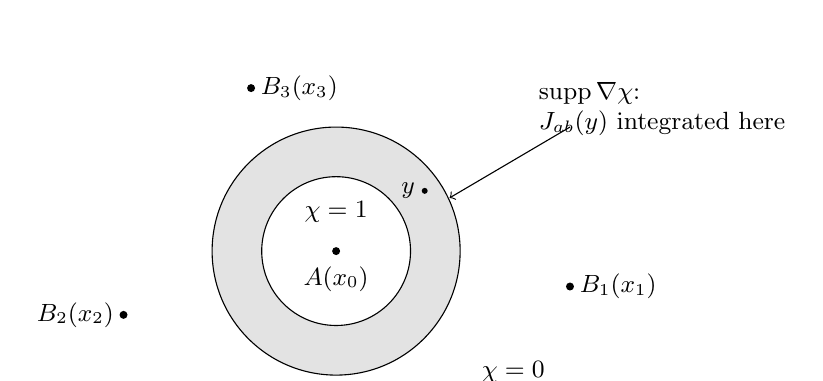
\begin{tikzpicture}[scale=0.9,font=\small]
\fill[gray!22,even odd rule] (0,0) circle (1.75) (0,0) circle (1.05);
\draw (0,0) circle (1.05); \draw (0,0) circle (1.75);
\fill (0,0) circle (1.6pt) node[below=2pt] {$A(x_0)$};
\node at (0,0.55) {$\chi=1$};
\fill (1.25,0.85) circle (1.2pt) node[left] {$y$};
\node[align=left] at (4.6,2.0) {$\operatorname{supp}\nabla\chi$:\\ $J_{ab}(y)$ integrated here};
\draw[->] (3.3,1.75) -- (1.6,0.75);
\fill (3.3,-0.5) circle (1.6pt) node[right] {$B_1(x_1)$};
\fill (-3.0,-0.9) circle (1.6pt) node[left] {$B_2(x_2)$};
\fill (-1.2,2.3) circle (1.6pt) node[right] {$B_3(x_3)$};
\node at (2.5,-1.7) {$\chi=0$};
\end{tikzpicture}
\caption{The shell flux of Definition~\ref{def:D13}. The cutoff~$\chi$ equals one near the insertion $A(x_0)$ and vanishes near the spectators $B_i(x_i)$; the current is integrated against $\nabla\chi$ on the shaded annulus. Conservation makes the flux independent of~$\chi$, so the annulus may shrink towards~$x_0$ or grow until it meets a spectator. It says nothing about flux through large spheres. The vanishing of the total angular flux at infinity is proved separately: on coordinate lines in Lemma~\ref{lem:G-collinear-flux}, and for all configurations in Lemma~\ref{lem:G3.1}.}
\label{fig:G-shell}
\end{figure}

The sign convention can be seen in one free example (Figure~\ref{fig:G-shell}). By Lemma~\ref{lem:G1.1}(iv), $\maxwellcorr_2(\curvaturesquare(x),\curvaturesquare(y))=c|x-y|^{-8}$ with $c=3\dimG/\pi^4$. The translation shell Ward identity~\eqref{eq:G-free-shells} and the free derivative law give, for a shell around~$x$,
\begin{equation*}
\mathcal P_b^{\maxwellstress}=\partial_{x_b}\bigl(c|x-y|^{-8}\bigr)=-8c\,(x_b-y_b)|x-y|^{-10}.
\end{equation*}
Replacing $\maxwellstress$ by $\lambda\maxwellstress$ multiplies this flux by~$\lambda$, so the requirement that the flux be the derivative fixes both the normalization and the sign of the stress tensor. This is a free-field calculation; nothing is asserted here about the form of interacting correlations.

The next lemmas concern only the invariant polynomial algebra of Definition~\ref{def:D11}, realized by the Taylor sections of Lemma~\ref{lem:A1}. A curvature jet of order~$j$ has weight~$j+2$. Let $\mathfrak P$ be the complex polynomial algebra on all on-shell jets, $\mathfrak P_{\le j}$ its subalgebra using orders at most~$j$, and $\mathfrak P^G$ the invariant subalgebra. The invariant polynomials of weight at most~$d$ identify with~$\maxwellspace{d}$. For a spectator degree~$d$ put
\begin{equation*}
\mathfrak N_d=\{P\in\mathfrak P:S^{\rm Max}(P(0),u_1(x_1),\ldots,u_n(x_n))=0
\text{ for all }n,\ u_i\in\maxwellspace{d},\ (0,x)\in\Conf{n+1}\},
\end{equation*}
with every polynomial Wick ordered at its own site. The degree of~$P$ is unrestricted. The next result says that spectators of one bounded degree detect every invariant polynomial, however high its jet order.
\begin{lemma}[Detection by bounded spectators]\label{lem:G-detection}
There is $d_0\in\N$ such that
\begin{equation}\label{eq:G-detection}
\mathfrak N_{d_0}\cap\mathfrak P^{G}=\{0\}.
\end{equation}
\end{lemma}
The proof has two stages. At a fixed jet order, finite generation and reflected positivity give a bound on the spectator degree. To make the bound independent of the jet order, a quadratic spectator isolates a highest-order jet derivative of~$P$ by its harmonic pole, and induction on weight removes that jet order.

The extraction rests on the difference between a single harmonic pole and a product of poles. In four dimensions $K(z)=\partial_1\partial_2|z|^{-2}=8z_1z_2|z|^{-6}$ is harmonic and homogeneous of degree $-4$; multiplication by $|z|^{4}$ leaves $8z_1z_2|z|^{-2}$, which is not analytic at zero, and only $|z|^{6}$ clears it. The product of two poles $|z|^{-2}\cdot|z|^{-2}=|z|^{-4}$ has the same degree but is already cleared by~$|z|^4$. In general a product of poles of orders $r_1,r_2\ge2$ is cleared by $|z|^{2(r_1+r_2-2)}$, while a harmonic pole of order $r_1+r_2$ needs $|z|^{2(r_1+r_2-1)}$.
\begin{proof}[Proof of Lemma~\ref{lem:G-detection}]
\emph{Step 1: bounded jet order.} Fix~$j$. The algebra~$\mathfrak P_{\le j}$ is a polynomial algebra on finitely many variables, hence Noetherian by the Hilbert basis theorem~\cite[Lemma~10.31.1]{Stacks2026}. Its ideal generated by invariant polynomials of positive ordinary degree therefore has finitely many invariant, ordinary-homogeneous generators~$f_\alpha$. Every invariant ordinary-homogeneous polynomial is a sum of products of invariant homogeneous polynomials of weight at most some~$b_j$: write $P=\sum a_\alpha f_\alpha$, keep only terms of total degree~$\deg P$, and replace $a_\alpha$ by its gauge average, whose degree is smaller; induction on the degree concludes.

Spectators of degree~$b_j$ detect: $\mathfrak N_{b_j}\cap\mathfrak P^G\cap\mathfrak P_{\le j}=\{0\}$. Otherwise take its lowest nonzero ordinary-homogeneous part~$P_r$ and split a product of homogeneous factors of total ordinary degree~$r$ into distinct nearby spectator sites. Every leg of~$P$ must pair with a spectator leg, so terms with internal spectator contractions, or with higher-degree parts of~$P$, vanish. As the spectator sites coalesce, Wick's rule gives the two-site pairing of~$P_r$ with their ordinary product. Each factor has weight at most~$b_j$, so for $P\in\mathfrak N_{b_j}$ this limit is zero. Choose the product sum to be the reflection of~$\overline{P_r}$; Lemma~\ref{lem:G1.1}(ii) makes this pairing strictly positive, a contradiction.

\emph{Step 2: pole extraction.} Put $g=\dimG$ and choose $d_0\ge\max\{b_g,2g+5\}$. In a real colour basis write $X_{j,\alpha}(p)$ for the jet coordinate tested by a scalar order-$j$ probe~$p$. For scalar probes~$p,q$ of orders $k,l$, the invariant quadratic $\sum_\alpha{:}X_{k,\alpha}(p)X_{l,\alpha}(q){:}$ has weight~$k+l+4$. Its collision with a polynomial using jets through order~$j$ has, in the coefficient where just the order-$k$ leg contracts at order~$j$, the polynomial
\begin{equation}\label{eq:G-collision}
\sum_\alpha X_{l,\alpha}(q)\sum_\mu
C_{k,j}(p,e_\mu;z)\frac{\partial P}{\partial X_{j,\alpha}(e_\mu)},
\end{equation}
where $(e_\mu)$ is a basis of order-$j$ probes and $C_{k,j}$ their differentiated curvature covariance.

\emph{Claim.} If $P\in\mathfrak N_{d_0}$, $l<k$ and $k+l+4\le d_0$, then~\eqref{eq:G-collision} lies in~$\mathfrak N_{d_0}$. Put $r=4+k+j$. Tested against fixed exterior spectators, the term~\eqref{eq:G-collision} is harmonic and homogeneous of degree~$-r$ in~$z$, so $|z|^{2(r-1)}$ times it is analytic at zero. The other terms, expanded in Taylor series at each singular order, give at order~$r$ homogeneous functions that become analytic after multiplication by $|z|^{2(r-2)}$: a double contraction is a product of poles of orders $r_1,r_2\ge2$, cleared by $|z|^{2(r_1+r_2-2)}$, and Taylor terms keep this improvement. The contraction of the order-$l$ leg alone has order at most $4+l+j<r$. The claim now follows from:
\begin{equation*}
\text{a harmonic $K$, homogeneous of degree $-r\le-2$, with $|z|^{2(r-2)}K$ analytic at $0$, vanishes.}
\end{equation*}
Indeed $\Delta(|z|^{2s}K)=4s(s+1-r)|z|^{2s-2}K$ in four dimensions; successive Laplacians show that~$K$ extends analytically, and negative homogeneity makes it zero. Expand the collision through an order exceeding $8+k+l+2j$. Since its correlation with the quadratic test and further bounded-degree spectators vanishes identically, comparing successive radial homogeneities makes the order-$r$ harmonic pole zero, so~\eqref{eq:G-collision} belongs to~$\mathfrak N_{d_0}$.

\emph{Step 3: induction on weight.} Take $k=g+1$ and $l=0,\ldots,g-1$. For each~$l$ choose a probe~$q_l$ and a jet value~$v_l$ with $q_l(v_l)=1$. The matrix $(X_{l,\alpha}(q_l))_{l,\alpha}$ has nonzero polynomial determinant: assigning~$v_l$ to colour~$l$ and zero to the other colours in order~$l$ makes it the identity. For $j>g$ the polynomial~\eqref{eq:G-collision} replaces an order-$j$ jet by an order-$l$ jet, so its weight is smaller, and the induction hypothesis makes it zero. Multiplication by the transposed cofactor matrix shows that every one-colour contraction in~\eqref{eq:G-collision} vanishes. As $z,p$ vary, the forms $C_{k,j}(p,\cdot;z)$ span the dual of the order-$j$ jets: their common annihilator generates a Maxwell wave whose order-$k$ jets vanish everywhere, a polynomial of degree below~$k$ with negative homogeneity, hence zero, and~\eqref{eq:G-kelvin} makes the probe zero. Hence every order-$j$ partial derivative of~$P$ vanishes. Descending from the top order removes all orders above~$g$; Step~1 with spectator bound~$b_g$ treats the rest.
\end{proof}

Let $\mathcal C_d$ be the real space of complex linear tuples $\mathsf X_a:\maxwellspace{d}\to\maxwellspace{d+1}$ that commute with conjugation, kill the unit, are vector-covariant under~$\hypercubic$, and send $\maxwellspace{e}$ into~$\maxwellspace{e+1}$ for $e\le d$. For $\mathsf X\in\mathcal C_d$ the Ward sum is
\begin{equation*}
\mathcal E_b(\mathsf X;\boldsymbol u,x)=\sum_i S_n^{\rm Max}(u_1,\ldots,\mathsf X_bu_i,\ldots,u_n;x).
\end{equation*}
Finitely many tests on lines determine its kernel.
\begin{lemma}[Finite vector Ward tests]\label{lem:G1-vector}
For all sufficiently large~$d$, finitely many positional derivatives of $\mathcal E_b(\mathsf X;\boldsymbol u,x)$, with $u_i\in\maxwellspace{d}$ and~$x$ on a coordinate line perpendicular to~$e_b$, define a real linear map~$\mathcal T_d$ with
\begin{equation}\label{eq:G-free-tests}
\ker\mathcal T_d=\R\partial^{\rm Max}\quad\text{in }\mathcal C_d.
\end{equation}
\end{lemma}
\begin{proof}
Take $d\ge d_0$ from Lemma~\ref{lem:G-detection}. Suppose all the stated jets of the Ward sums of~$\mathsf X$ vanish.

\emph{Step 1: continuation off the lines.} Free correlations are real analytic off the diagonals by~\eqref{eq:G-curvature}, so every Ward sum vanishes near each testing line. For a separated configuration choose distinct ordered line coordinates respecting the strict order of its coordinates in that axis. The straight segment to the line configuration stays separated: strict inequalities persist, and coordinate ties are separated by the line coordinates. Analytic continuation along it gives $\mathcal E_b=0$ on~$\Conf{n}$.

\emph{Step 2: weight four.} Let $\mathsf J_j$ be the scalar on-shell order-$j$ jet space. For $p\in\mathsf J_0^*$ put $U(p)=\sum_\alpha{:}X_{0,\alpha}(p)^2{:}$. Simplicity, the filtration and inversion parity force $\mathsf X_bU(p)$ to be a colour contraction of one order-zero and one order-one jet, represented by a linear map $A_p:\mathsf J_0\to\mathsf J_1^*$. In the Ward identity of $U(p),U(q),U(w)$ let the first two points coalesce along~$tu$ and multiply by~$t^5$. The term with $\mathsf X_b$ at the distant point tends to zero, and the two remaining triangular Wick contractions give, for every $X\in\mathsf J_0$ and with $C_{1,0}$ taken in one colour,
\begin{equation*}
C_{1,0}(A_pX,q;u)\,q(X)=C_{1,0}(A_qX,p;u)\,p(X).
\end{equation*}
Arbitrary~$X$ are reached by choosing the distant probe~$w$ through the invertible order-zero covariance~\eqref{eq:G-kelvin}. If $p(X)=0$, choose $q(X)\ne0$; varying $q,u$ gives $A_pX=0$. Thus $A_pX=p(X)f_bp$, and the same identity shows that $f_b:\mathsf J_0^*\to\mathsf J_1^*$ is real linear with $C_{1,0}(f_bp,q;u)=C_{1,0}(f_bq,p;u)$.

\emph{Calculation of~$f_b$.} Write $e^{ij}$ for the curvature coordinate and $\partial_he^{ij}$ for its first jet. For $f_1e^{12}$, sign parity permits only $\partial_1e^{12},\partial_3e^{23},\partial_4e^{24}$; interchange of axes~$3,4$ and $\sum_i\partial_ie^{i2}=0$ reduce their span to $\R\partial_1e^{12}$. For $f_1e^{23}$ the candidates $\partial_1e^{23},\partial_2e^{13},\partial_3e^{12}$ reduce, by antisymmetry in axes~$2,3$ and Bianchi, to $\R\partial_1e^{23}$. Permutations leave two constants, which agree because $C_{1,0}(\partial_1e^{12},e^{23};e_1+e_3)=-1/(2\pi^2)\ne0$ by~\eqref{eq:G-curvature}. Therefore $f_b=c_{\rm jet}\partial_b$, and since $\partial_bU(p)$ has two identical terms, $\mathsf X_b=c\,\partial^{\rm Max}_b$ on weight four with $c=c_{\rm jet}/2$.

\emph{Step 3: higher weights.} Set $\mathsf X^\circ_b=\mathsf X_b-c\,\partial^{\rm Max}_b$. Translation invariance makes its Ward sums zero, and it kills every free stress component. Insert into such a sum a free stress shell for the dilation field $v(y)=y-x_0$, surrounding only the distinguished point. The term where $\mathsf X^\circ_b$ acts on the stress is zero. The other shell terms are given by the polarized calculation in Lemma~\ref{lem:G1.1}, now with this~$v$; the extra derivative of~$v$ contracts with the trace of the free stress, which is zero by~\eqref{eq:G-free-tensor}. The local Lie derivative of a two-form under dilation is $y\cdot\nabla+2$, and on jets it gives the weight operator $\mathsf D^{\rm wt}X_{j,\alpha}=(j+2)X_{j,\alpha}$. Subtracting the Ward sum with distinguished label~$\mathsf D^{\rm wt}u$ shows $[\mathsf D^{\rm wt},\mathsf X^\circ_b]u\in\mathfrak N_d$, and Lemma~\ref{lem:G-detection} makes it zero. So $\mathsf X^\circ_b$ preserves each weight. Inversion acts there by~$(-1)^{\rm weight}$, whereas vector covariance makes $\mathsf X^\circ_b$ odd under inversion; hence $\mathsf X^\circ_b=0$.

\emph{Step 4: finite selection.} Conversely translation invariance annihilates every test on~$\partial^{\rm Max}$. The real space~$\mathcal C_d$ is finite-dimensional; successively choose a test nonzero on the current kernel modulo this line. Each choice lowers its dimension, so finitely many tests have precisely the asserted kernel.
\end{proof}

The internal tests rest on one elementary fact about the plane generators $K_{ab}=E_{ba}-E_{ab}$ of $\mathfrak{so}(4)$. Call a coordinate quarter turn the rotation $e_a\mapsto e_b$, $e_b\mapsto-e_a$ in one coordinate plane.
\begin{lemma}[Alternating planes]\label{lem:G-planes}
Let $\beta:\mathfrak{so}(4)\times\mathfrak{so}(4)\to V$ be real bilinear and alternating, with $\beta(hKh^{-1},hLh^{-1})=\beta(K,L)$ for every coordinate quarter turn~$h$. Then $\beta=0$.
\end{lemma}
\begin{proof}
The quarter turns generate the determinant-one signed permutations: they project onto the transpositions of $S_4$, and squares of quarter turns give the diagonal sign changes with two minus signs. Conjugation by a diagonal sign matrix~$s$ multiplies $K_{ab}$ by $s_as_b$; conjugation by a permutation matrix permutes the planes. \emph{Overlapping planes:} $s=\operatorname{diag}(1,1,-1,-1)$ fixes $K_{12}$ and reverses the sign of $K_{13}$, so $\beta(K_{12},K_{13})=-\beta(K_{12},K_{13})=0$. \emph{Disjoint planes:} the even permutation $(13)(24)$ interchanges $K_{12}$ and $K_{34}$, so $\beta(K_{12},K_{34})=\beta(K_{34},K_{12})=-\beta(K_{12},K_{34})=0$. Every pair of distinct planes is carried to one of these two pairs by a signed permutation of determinant one, and $\beta(K,K)=0$; bilinearity gives $\beta=0$.
\end{proof}

Let $\mathcal B_d$ consist of alternating real-bilinear families $\Delta:\mathfrak{so}(4)^2\to\operatorname{End}_{\C}\maxwellspace{d}$ which commute with conjugation, kill the unit, preserve every lower-degree subspace, and satisfy
\begin{equation*}
R^{\rm Max}(h)\Delta(K,L)=\Delta(hKh^{-1},hLh^{-1})R^{\rm Max}(h)
\qquad(h\in\hypercubic,\ \det h=1).
\end{equation*}
The next result removes the defect in the rotation commutator.
\begin{lemma}[Finite internal Ward tests]\label{lem:G1-internal}
For every $d\ge4$, finitely many sums
\begin{equation}\label{eq:G-erasure-test}
\sum_i S_n^{\rm Max}(u_1,\ldots,\Delta(K,L)u_i,\ldots,u_n;x),
\qquad u_i\in\maxwellspace{d},\quad x\in\Conf{n},
\end{equation}
separate~$\mathcal B_d$.
\end{lemma}
\begin{proof}
Suppose all these sums vanish and fix $\mathsf Z=\Delta(K,L)$. On the weight-four space let $b_x(u,v)=S_2^{\rm Max}(u,v;x,0)$. The order-zero Kelvin formula and Wick's rule give $b_x(u,v)=b_y(R^{\rm Max}(\mathcal R_y\mathcal R_x)u,v)$ for $|x|=|y|\ne0$. Both $\mathsf Z$ and the orthogonal action preserve this space. Applying $b_x(\mathsf Zu,v)+b_x(u,\mathsf Zv)=0$ at~$x$ and~$y$, and nondegeneracy of~$b_y$, shows that~$\mathsf Z$ commutes with $R^{\rm Max}(\mathcal R_y\mathcal R_x)$, in particular with every coordinate quarter turn. With the signed covariance of~$\Delta$, the function $(K,L)\mapsto\Delta(K,L)u$ satisfies the hypothesis of Lemma~\ref{lem:G-planes} for each weight-four~$u$, so~$\mathsf Z$ vanishes on weight four, including the stress.

Insert a free angular stress shell around the distinguished point only, as in Step~3 of the proof of Lemma~\ref{lem:G1-vector}. Subtracting the Ward sum with the angularly differentiated label gives $[\mathsf L^{\rm Max}(M),\mathsf Z]u\in\mathfrak N_d$. This polynomial has weight at most~$d$, so Lemma~\ref{lem:G1.1}(ii) makes it zero. Hence $\mathsf Z$ commutes with all infinitesimal rotations, and differentiating $e^{t\mathsf L(M)}\mathsf Z-\mathsf Ze^{t\mathsf L(M)}$ gives commutation with coordinate quarter turns in every degree. Lemma~\ref{lem:G-planes} again gives $\Delta=0$. Finite-dimensionality selects a finite separating subfamily by successively reducing the common kernel.
\end{proof}

\subsection{Lattice inputs}\label{sec:G-lattice}

The insertions are those of Definition~\ref{def:D08}, with coefficient polynomials from Definition~\ref{def:D19} and Lemma~\ref{lem:A1}. The inverse coefficient estimate of Lemma~\ref{lem:E-marked-step} inverts the marked coefficient map; the corrected sources and normalized integral of Lemmas~\ref{lem:E-Gaussian-sources} and~\ref{lem:E-source-integral} bound the remainders; the uniform displacement estimate of Lemma~\ref{lem:E-displacement} controls positions, with coordinate separations at least four times the displacement margin. Chessboard seminorms are those of Definition~\ref{def:D27}. Cutoff limits are taken in the order~\eqref{eq:E2-tails}, followed by the fixed extraction of Lemma~\ref{lem:F1}; an ordered limit point of a bounded coefficient family is its limit along an ultrafilter containing the ordered tails.

Fix arity and degree bounds $n\ge2,D\ge1$ and $R\ge1$. A basis word is a list of members of fixed real bases of $\maxwellspace{d}$, $d\le D$. Put
\begin{equation*}
K_{R,m}=\{x:|x|\le R,\ \sepinf(x)\ge R^{-1}\},\qquad
E_\delta=\{x:|x_i^a-x_j^a|>\delta\ (i\ne j,\ a=1,\ldots,4)\}.
\end{equation*}
The comparison exponents $\alpha_0,\alpha_1,\alpha_2>0$ and $c<0$ have the following roles: $\alpha_0$ sets the comparison radius, $\alpha_1$ the cells used for moment bounds, $\alpha_2$ the smaller cells used for displacement bounds, and~$c$ the width of the excluded coordinate strips. They satisfy
\begin{equation}\label{eq:G-exponents}
\alpha_1+6<\alpha_0,\quad \alpha_2+5<\alpha_0+c,\quad
(\alpha_0-\alpha_1)Dn+c<0,\quad
(\alpha_0-\alpha_2)Dn-\alpha_0-c<0.
\end{equation}
The first two inequalities place the chessboard cells; the last two make the excluded strips negligible. One explicit choice, with $n_{\max}=\max(n,D)$, is $\kappa_1=7n_{\max}(n_{\max}+2)+1$, $\kappa_2=6+\kappa_1$, $\alpha_0=17+n_{\max}+\kappa_1+\kappa_2n_{\max}(n_{\max}+2)+\kappa_2$, $\alpha_1=\alpha_0-7$, $\alpha_2=\alpha_0-\kappa_2$ and $c=-\kappa_1$. Write $M_k=\cutoffsize_k$ and set
\begin{equation}\label{eq:G-balance}
r_k=a_kM_k^{\alpha_0},\qquad \mathfrak s_k=M_k^{-\alpha_0},\qquad
\delta_k=M_k^{c},\qquad
R^{\rm cell}_k=CM_k^{(\alpha_0-\alpha_1)D},\quad R^{\rm var}_k=CM_k^{(\alpha_0-\alpha_2)D},
\end{equation}
where $C\ge1$ depends only on $n,D,R$ and the construction and is fixed in the proof of Lemma~\ref{lem:G-lattice}. Thus $r_k\mathfrak s_k=a_k$: the normalized grid is the physical construction grid. For an ordered limit point $c_{k,d}:\maxwellspace{d}\to V_d$ of the lifts in Lemma~\ref{lem:G-lattice}, and the quotient $\pi_d:V_d\to F_d$ of Definition~\ref{def:D10}, define the rescaled correlation
\begin{equation*}
S^{\rm sc}_k(\boldsymbol u;x)=S_m(\pi_{d_i}c_{k,d_i}u_i;r_kx).
\end{equation*}

The following comparison uses one coefficient family for every word within the fixed bounds. Its constants may depend on these bounds, the word and the construction. The arity, degree and radius bounds are fixed first, then the level and the lifts; the estimates then hold for every basis word within these bounds.
\begin{lemma}[Lattice comparison at small radii]\label{lem:G-lattice}
There are arbitrarily large levels~$k$, real $\hypercubic$-equivariant lifts $\Lambda_{k,N,p,d}:\maxwellspace{d}\to V_d$ preserving the degree-zero unit, and $\varepsilon_k\to0$ such that every ordered limit point of these lifts satisfies, for every basis word with $m\le n$,
\begin{equation}\label{eq:G-lattice-input}
\begin{aligned}
|S^{\rm sc}_k|&\le (R^{\rm cell}_k)^m &&\text{on }K_{R,m},\\
\|\nabla S^{\rm sc}_k\|&\le4m (R^{\rm var}_k)^m/\delta_k &&\text{on }K_{2R,m}\cap E_{4\delta_k},\\
|S^{\rm sc}_k-S_m^{\rm Max}|&\le\varepsilon_k
&&\text{on }(\mathfrak s_k\Z)^{4m}\cap K_{2R,m}\cap E_0.
\end{aligned}
\end{equation}
At fixed~$k$ the lifts are bounded on ordered tails.
\end{lemma}
The lifts are chosen so that the rescaled insertions have the free Wick polynomials as Gaussian leading part~\eqref{eq:G-lift-equation}. A subset recursion removes the continuum Gaussian moments; for exact Gaussian variables each remainder has mean zero, and the source estimates of Section~\ref{sec:partII-E} make each remainder small in chessboard seminorm~\eqref{eq:G-source-root}. The chessboard inequality then gives the comparison on the grid, and the coarser normalizations $\alpha_1,\alpha_2$ give the size and gradient bounds off the grid.
\begin{proof}
\emph{Step 1: lifts.} Choose a real $\hypercubic$-equivariant polynomial representative map $\iota_d^{\rm free}$ for the on-shell quotient, using the Taylor sections of Lemma~\ref{lem:A1} and averaging a real splitting over~$\hypercubic$. Let $\mathsf C_{k,N,p,d}$ be the marked coefficient map from level~$k$ down to~$\reflevel{d}$, after the Wick-ordering correction of Lemma~\ref{lem:E-source-polynomial}. Write $\delta_t^{\rm wt}$ for multiplication of a weight-$j$ monomial by~$t^j$; the factor-count scaling~$t^{\factorcount}$ is that of Definition~\ref{def:D08}. The Gaussian field divided by the small-field threshold has scale
\begin{equation*}
\mathfrak t_{k,N,p}=(t_k\sqrt{\beta_{N,p,k}})^{-1},\qquad
0<\mathfrak t_{k,N,p}^{-1}\le2M_k,
\end{equation*}
since $t_k=M_k/\sqrt{\refbeta_k}$ is the small-field threshold of Part~I and $\beta_{N,p,k}\le2\refbeta_k$. Solve
\begin{equation}\label{eq:G-lift-equation}
\mathsf C_{k,N,p,d}\Lambda_{k,N,p,d}u
=\mathfrak t_{k,N,p}^{-\factorcount}\delta_{M_k^{\alpha_0}}^{\rm wt}\iota_d^{\rm free}u.
\end{equation}
The solution exists and obeys
\begin{equation}\label{eq:G-lift-bound}
|v|_1\le K_{k,d}a_k^d|\mathsf C_{k,N,p,d}v|_1,
\end{equation}
with $K_{k,d}$ independent of~$N,p$ at fixed~$k$. Indeed, apply the inverse estimate of Lemma~\ref{lem:E-marked-step} at each step $m+1\to m$ from level~$k$ down to~$\reflevel{d}$, and the coefficient comparison in the proof of Lemma~\ref{lem:E-source-polynomial}, whose relative error is less than~$1/4$, so its inverse costs at most~$2$. One may take $K_{k,d}$ to be twice the product of the finitely many column and block factors up to~$k$, enlarged by the fixed basis norms. The coefficient map is injective, hence invertible on its finite coefficient space, and its unit, conjugation and signed laws pass to the inverse. The bound on~$\mathfrak t^{-1}$ bounds the right side at fixed~$k$, so the lifts are bounded on cutoff tails.

\emph{Step 2: subset recursion.} Lemmas~\ref{lem:E-source-polynomial}--\ref{lem:E-source-integral} hold for an arity bound~$n\ge2$, at most~$n$ marks per cell and any compact position set with positive point separation; apply them to the interval~\eqref{eq:E-window} with exponent~$\alpha_0$ and position set~$K_{2R,m}$. Their covariance and Taylor bounds are uniform on $K_{2R,m}$, whose point separations are at least $(2R)^{-1}$, and need no lower bound on coordinate differences; only the reflected placement below requires~$E_0$. Write $I_i=O_{N,p}^{(d_i)}(\Lambda_{k,N,p,d_i}u_i,r_kx_i/a_N)$ at compatible lattice points. For a subset~$J$ put $G_J=S_{|J|}^{\rm Max}((u_i)_{i\in J};(x_i)_{i\in J})$ and define
\begin{equation*}
R_\varnothing=1,\qquad
R_I=\prod_{i\in I}I_i-\sum_{\varnothing\ne J\subseteq I}G_JR_{I\setminus J}.
\end{equation*}
This subtracts the full continuum Gaussian moment on every subset of slots; for exact continuum Gaussian variables its nonempty coefficients have expectation zero, by induction on~$|I|$. The Wick-ordering correction and~\eqref{eq:G-lift-equation} identify the leading Gaussian correlations with these continuum moments at the normalized grid points, as calculated in Lemma~\ref{lem:E-source-polynomial}. Covariance, Taylor and localization errors remain in the regular and forced source terms.

\emph{Step 3: chessboard seminorm of the remainders.} The finite-set clause of Lemma~\ref{lem:E1.1} gives arbitrarily late common terminal levels~$k$ for the three exponents $\alpha_0,\alpha_1,\alpha_2$. Use the interval~\eqref{eq:E-window} with exponent~$\alpha_0$, its width level $w_{\alpha_0}(k)=k-h_k(\alpha_0)-v_k$ and its centered tiling $\mathcal C^{\rm tile}_{w_{\alpha_0}(k)}(0)$. Put $q_k=\log M_k/(16n)$ and give each mark weight $e^{2q_k}\le M_k^{1/16}$. The weighted mode norm in the proof of Lemma~\ref{lem:E-replication} multiplies mark weights over subsets, so coefficient extraction for a nonempty~$I$ contributes $e^{-2q_k|I|}$ in each reflected cell, and the corrected-source iteration of Lemma~\ref{lem:E-Gaussian-sources} keeps this mark weight on the selected comparison intervals. Work in $\C[z_1,\ldots,z_m]/(z_i^2)$ and multiply by the reciprocal of the continuum free moment polynomial; its coefficient of~$z_I$ is exactly~$R_I$. After the finite Gaussian contractions on every subset, the remaining source modes have zero leading Gaussian coefficient. In the source iteration, terms linear in these modes cost the finite stage constant, and every other connected term contains at least two residual modes and is bounded by their squared norm times a fixed power of~$M_k$; this is~\eqref{eq:E-source-step}. The covariance and localization errors of Lemma~\ref{lem:E-source-polynomial} are below the corresponding source tolerance at entry~\eqref{eq:E-source-iteration}. Lemma~\ref{lem:E-Gaussian-sources}, applied to the coefficients~\eqref{eq:E-corrected-coefficients} of these finitely many subset modes, gives this mark weight with constants depending only on $n,D,R$ and the construction; its sums are rooted at a mark and do not count the replicated cells.

The normalized positive integral costs, per cell, at most the stage constant $Q_{J_k}^{\rm cmp}$ of~\eqref{eq:E-comparison-cost} (Lemma~\ref{lem:E-source-integral}), which contains the term $1+n$ for at most~$n$ marks. Item~\ref{it:E-entries} imposes $Q_j^{\rm cmp}\le\log M_t/(16n)$ for each arity bound, hence $Q_{J_k}^{\rm cmp}\le q_k$; the entry is chosen after the finitely many source constants. Taking the root over the reflected cells gives
\begin{equation}\label{eq:G-source-root}
\|R_I\|_{\mathcal C^{\rm tile}_{w_{\alpha_0}(k)}(0)}
\le e^{q_k-2q_k|I|}\le M_k^{-1/(16n)}
\qquad(\varnothing\ne I\subseteq\{1,\ldots,m\}).
\end{equation}
The smallness comes from the corrected density at large coupling: its source terms stay bounded at a growing mark weight, while the unmarked normalization grows more slowly than that weight. The estimate concerns the complete reflected array, before absolute values are taken, and needs no independence of the insertions.

\emph{Step 4: comparison on the grid.} Distinct coordinate differences at normalized grid points are at least $\mathfrak s_k$, so their physical differences are at least~$a_k$. The reading map assigns the corresponding level-$k$ sites without rounding, and the interval margin~\eqref{eq:E-window-geometry} contains the inspected stencils and their reflected copies. Expanding the recursion, applying~\eqref{eq:E-chess} to each~$R_I$ and bounding the free submoments on~$K_{2R,m}$ gives $C_{R,\boldsymbol u}M_k^{-1/(16n)}$, the last line of~\eqref{eq:G-lattice-input}.

\emph{Step 5: size and variation off the grid.} At its own normalization the singleton comparison gives a chessboard seminorm at most $1+|S_1^{\rm Max}(u)|$. For exponent~$\alpha_1$, changing normalization to~$M_k^{\alpha_0}$ multiplies a weight-$j$ coefficient by $M_k^{(\alpha_0-\alpha_1)j}$, so the finite coefficient sum bounds these seminorms by~$R^{\rm cell}_k$ for~$C$ large; exponent~$\alpha_2$ gives~$R^{\rm var}_k$. Include every reflected basis label and its complex conjugation in these maxima. The two interval lengths of~\eqref{eq:E-window} give, with the stage block ratio~$L$,
\begin{equation}\label{eq:G-root-sides}
\frac{a_{w_b(k)}}{a_k}=L^{h_k(b)+v_k}
\le L^2M_k^{b+2}B_k^{10}\le M_k^{b+5}
\qquad(b=\alpha_1,\alpha_2),
\end{equation}
after the stage entry, where $L$ is fixed and $B_k=M_k^{o(1)}$. So the $\alpha_1$ cell is at most $a_kM_k^{\alpha_1+6}=o(r_k)$ and the $\alpha_2$ cell is $o(r_k\delta_k)$ by~\eqref{eq:G-exponents}. The chessboard inequality bounds separated continuum moments by~$(R^{\rm cell}_k)^m$. The physical diameter on~$r_kK_{2R,m}$ is at most $4Rr_k<L_p/2$ on the ordered tails, so the torus separation~$g_p$ of Lemma~\ref{lem:E-displacement} is the minimum ordinary coordinate separation, which exceeds $4r_k\delta_k$ on~$E_{4\delta_k}$. The uniform clause of Lemma~\ref{lem:E-displacement}, with margin $r_k\delta_k$ and the reflected seminorms included in~$R^{\rm var}_k$, gives $4m(R^{\rm var}_k)^m/\delta_k$ after rescaling. The three normalizations use the same coefficient map and lifts and the same terminal levels; the finitely many cutoff tails can be intersected.

\emph{Step 6: limits.} Take any ordered limit point of the bounded lifts. Lemma~\ref{lem:E3.1} and~\eqref{eq:F-conf} pass the moment estimates to the fixed table, and Proposition~\ref{prop:FC} with Lemma~\ref{lem:F2} passes the difference bound. No extraction of the table or the volume sequence is made.
\end{proof}

For the shell estimate take $\varkappa\in\{0,1\}$, $A\in F_d$, $B\in F_4$ and $D=d+1-\varkappa$. The shell factor has scaling degree $3+\varkappa$: integration over four dimensions contributes four powers of the radius, the differentiated cutoff removes one, and the constant or linear vector field contributes~$\varkappa$. Since the two inserted fields have total degree $d+4$, the expected output degree is $(d+4)-(3+\varkappa)=D$. A grid test is a separated configuration $(0,x_i)$ on $a_{j_0}\Z^4$ for some level~$j_0$, generic in each coordinate, with a fixed spectator list~$\boldsymbol B_i$. Its response functional and marked response are
\begin{equation*}
\mathsf r_i(v)=S(v(0),\boldsymbol B_i(x_i)),\qquad
\mathfrak h_i(y)=S(B(y),A(0),\boldsymbol B_i(x_i)).
\end{equation*}
Finite collections may use different grids, and the union of all these configurations is dense. The next lemma shows that every finite combination of tests annihilating $F_D$ also annihilates the limiting shell response.
\begin{lemma}[Annular annihilator estimate]\label{lem:G-annular}
For every finite list of grid tests and coefficients $g_i\in\C$ with $\sum_i g_i\mathsf r_i=0$ on~$F_D$, there are $\rho_l\downarrow0$ such that
\begin{equation}\label{eq:G-annular-input}
\sup_{1/4\le|z|\le2}\left|\sum_i g_i\rho_l^{3+\varkappa}\mathfrak h_i(\rho_lz)\right|\longrightarrow0.
\end{equation}
\end{lemma}
\begin{proof}
The local sections of Lemma~\ref{lem:A1} and Lemmas~\ref{lem:E2.2}--\ref{lem:E2.3} represent the product of two nearby marked insertions by one marked insertion of degree~$D$; Proposition~\ref{prop:FC} and Lemma~\ref{lem:F2} pass to the quotient. Put $h=3+\varkappa$, so $D+h=d+4$. Recall $s_m=\log(a_m^{-1})$ from~\eqref{eq:I12-levels}. Use the support radius $B_m=\lceil(\log\refbeta_m)^2\rceil$ of Part~I and take $\rho_m=128B_{m+1}^2a_{m+1}$, so $\log\rho_m=-s_m+o(s_m)$.

\emph{Step 1: two-mark representation.} Fix a centered cell around the distinguished point, disjoint from all spectator stencils, and a finer stopping level~$k_0\ge\reflevel{D}$ at which its replicated source estimate applies. Choose levels~$j(m)$ with
\begin{equation*}
\frac{s_{j(m)}}{s_m}\longrightarrow t=1+\frac1{64(d+12)};
\end{equation*}
they exist since $s_{m+1}/s_m\to1$ (Lemma~\ref{lem:E1.1}). At a grid point $y\in a_{j(m)}\Z^4$ with $\rho_m/16<|y|<4\rho_m$, choose representatives $a\in V_d,b\in V_4$ of~$A,B$, block their two marked insertions at~$y,0$ together, and retain the Taylor terms of weight at most~$D$. Their coefficient vector~$c_{N,p}(y)\in V_D$ is chosen by inverting the marked coefficient map. The exact difference is
\begin{equation*}
\rho_m^h O_{N,p}^{(4)}(b,y/a_N)O_{N,p}^{(d)}(a,0)
 -O_{N,p}^{(D)}(c_{N,p}(y),0).
\end{equation*}
Let $u_{m,1},u_{m,2}$ be the available mark weights of the degree-$d$ and rescaled degree-four marks at level~$j(m)$. The one-mark bounds, including~$\rho_m^h$, give $\log u_{m,1}=(-dt+o(1))s_m$ and $\log u_{m,2}=(-4t+h+o(1))s_m$; support weights, coefficient columns and threshold powers have logarithm~$o(s_m)$ by~\eqref{eq:E-marker-scales} and~\eqref{eq:E-log-cost}. Transporting each source to level~$m+1$ adds the volume factor $(a_{j(m)}/a_{m+1})^4$ to its weight. So the joint weight~$v_m$ and the dimensionless coefficient bound~$e_m$ of its Taylor remainder satisfy
\begin{equation}\label{eq:G-annular-cost}
\log v_m=[-D-(d+12)(t-1)+o(1)]s_m,\qquad
e_m\le\exp\{[(d+12)(t-1)+o(1)]s_m\}.
\end{equation}
Indeed the transported exponents sum to $-(d+4)t+h+8(1-t)=-D-(d+12)(t-1)$, and Taylor extraction costs the reciprocal joint weight times~$a_{m+1}^D$, which cancels the~$D$ term. This is the two-mark use of the source representation~\eqref{eq:E-source-form}, retaining its forced terms and their eligibility tests.

\emph{Step 2: backward matching.} Apply~\eqref{eq:E-backward-match-level} from~$m+1$ to the fixed stopping level~$k_0$. The matched remainder gains $\prod_{i=k_0}^{m}\ell_i^{1/8}=e^{(s_{m+1}-s_{k_0})/8}\ge e^{(s_m-s_{k_0})/8}$ in its inverse bound. Put $c_m=e^{s_m/32}$ and multiply the source by~$c_m$; its size is then at most
\begin{equation*}
c_me_me^{-(s_m-s_{k_0})/8}
\le\exp\{[-5/64+o(1)]s_m\},\qquad
\tfrac1{32}+(d+12)(t-1)-\tfrac18=-\tfrac5{64},
\end{equation*}
which eventually fits every fixed source allowance at~$k_0$. The residual-source estimate~\eqref{eq:E-residual-root} at the fixed cell and level~$k_0$ then bounds the chessboard seminorm of the unamplified residual by~$2C/c_m$, with~$C$ independent of~$m,N,p$. The inverse estimate~\eqref{eq:G-lift-bound} in degree~$D$ bounds~$c_{N,p}(y)$ on cutoff tails for each fixed~$m,y$. Interior support follows from $32\rho_m\to0$ and the support diameter $a_{m+1}(B_{m+1}^2+1+2048B_{m+1}^2)\to0$.

\emph{Step 3: cancellation at grid points.} Pass to an ordered limit point~$c(y)$ and project it to~$F_D$. The chessboard inequality~\eqref{eq:E-chess} for the residual and the fixed exterior stencils gives, simultaneously for the finite tests,
\begin{equation*}
|\rho_m^h\mathfrak h_i(y)-\mathsf r_i(\pi_Dc(y))|\le C_i c_m^{-1},
\end{equation*}
with the same coefficient vector for every spectator. Multiplication by~$g_i$ and summation cancel the response term, so $f_m(y)=\sum_i g_i\rho_m^h\mathfrak h_i(y)$ is $O(c_m^{-1})$ at all grid points of the enlarged annulus whose four coordinates are nonzero.

\emph{Step 4: interpolation across coordinate planes.} For a derivative order~$q$, Proposition~\ref{prop:FC} replaces the moving label by one of degree $4+q$. The centered and reflected bounds of Lemmas~\ref{lem:E2.3} and~\ref{lem:E-replication}, with~\eqref{eq:E-chess}, bound a field of fixed degree~$e$ by $\exp[(e+2+o(1))s_m]$, with a field-dependent constant of logarithm~$o(s_m)$. The finitely many later levels required for the fixed spectator word have logarithmic scale $s_m+o(s_m)$. Choose degree bounds~$e_{ij}$ for the spectator labels and put $C_0=8+d+\max_i\sum_j(e_{ij}+2)$. Since $\rho_m^h\le1$,
\begin{equation}\label{eq:G-annular-derivatives}
|\partial_a^q f_m(y)|\le \exp[(q+C_0+o(1))s_m]
\qquad(\rho_m/16<|y|<4\rho_m),
\end{equation}
with $C_0$ independent of~$q$. Choose $q$ with $q(t-1)>C_0$; since $a_{j(m)}=\exp[-(t+o(1))s_m]$, the $q$th derivatives along grid-sized segments tend to zero. On each coordinate segment of length $4(2^q+2)a_{j(m)}$ choose $q$ grid nodes with nonzero coordinates, mutually separated by at least $a_{j(m)}$. Lagrange interpolation gives $|g|\le C_q(\max_{\rm nodes}|g|+a_{j(m)}^q\sup|\partial^qg|)$ on the segment, with $C_q$ independent of~$m$. Apply it to ${\rm Re}\,f_m$ and ${\rm Im}\,f_m$ in each of the four axes; the segments stay in the enlarged annulus since $4(2^q+2)a_{j(m)}=o(\rho_m)$. Four successive interpolations give $\sup_{\rho_m/4\le|y|\le2\rho_m}|f_m(y)|\to0$. Select a decreasing subsequence of~$\rho_m$; it depends on the fixed tests and~$g$, as allowed.
\end{proof}

\subsection{Free comparison and the conserved line}\label{sec:partII-G.2}

The next lemma converts Lemma~\ref{lem:G-lattice} into the comparison of Part~I, measured uniformly over the supremum-norm unit ball of tests. No volume refinement is needed.
\begin{lemma}[Stable weak comparison]\label{lem:G2.1}
There is one stable scaling sequence such that, for every arity~$n$, degree list, $u_i\in\maxwellspace{d_i}$ and compact $\mathcal K\subset\Conf{n}$,
\begin{equation*}
\sup_{\|f\|_\infty\le1,\ \operatorname{supp}f\subset\mathcal K}\left|\int f(x)\bigl[S_n(\scaleframe{k}{d_i}u_i;r_kx)-\maxwellcorr_n(\boldsymbol u;x)\bigr]dx\right|\longrightarrow0.
\end{equation*}
\end{lemma}
\begin{proof}
Lemma~\ref{lem:G-lattice} supplies the three estimates, Lemma~\ref{lem:G1.1} the free modulus of continuity and the free separating tests, and Proposition~\ref{prop:FC} the dimension bound. The set $K_{R,m}\setminus E_{8\delta_k}$ lies in finitely many strips about coordinate coincidence hyperplanes and has volume at most $C_{m,R}\delta_k$; its contribution to a tested difference is at most $C_{m,R}\|f\|_\infty((R^{\rm cell}_k)^m+\|\maxwellcorr_m\|_{K_{R,m}})\delta_k$. Outside these strips, rounding to the grid moves a point by at most $4m\mathfrak s_k\le\delta_k$, so the segment stays in $K_{2R,m}\cap E_{4\delta_k}$. The mean value bound and the free modulus of continuity~$\varpi$ give total tested error at most
\begin{equation}\label{eq:G-tested-error}
C_{m,R}\|f\|_\infty
 \bigl[\varepsilon_k+((R^{\rm cell}_k)^m+\|\maxwellcorr_m\|_{K_{R,m}})\delta_k
       +(R^{\rm var}_k)^m\mathfrak s_k/\delta_k+\varpi(4m\mathfrak s_k)\bigr].
\end{equation}
Every term tends to zero by the strict inequalities~\eqref{eq:G-exponents}: the strips cost $(R^{\rm cell}_k)^m\delta_k$, the rounding costs $(R^{\rm var}_k)^m\mathfrak s_k/\delta_k$, and both are negative powers of~$M_k$. Arbitrary fields expand in the finitely many basis words, with coefficient sums bounded by the product of their norms.

At a fixed comparison level the lifts are bounded in a finite-dimensional space. Take an ordered limit point and project to~$F_d$; ordered convergence holds also for convergent coefficients, by multilinearity. This proves~\eqref{eq:G-tested-error} for linear maps $U_{k,d}:\maxwellspace{d}\to F_d$, for every ordered limit point and the same table (Lemma~\ref{lem:F1}).

Choose successively arity, degree and radius bounds tending to infinity, tolerances tending to zero, and strictly decreasing radii tending to zero; this is possible because $\log M_k=o(\log a_k^{-1})$ by~\eqref{eq:I12-scales} and~\eqref{eq:E-running}, whence $a_kM_k^{\alpha_0}\to0$. The sequence is selected before any field list. To impose inclusions exactly, choose real $\hypercubic$-equivariant left inverses $L_d$ of the free inclusions~$i_d$ and replace the maps recursively by
\begin{equation}\label{eq:G-correct-frames}
\widetilde U_{k,0}=U_{k,0},\qquad
\widetilde U_{k,d+1}=\jmath_{d,d+1}\widetilde U_{k,d}L_d
 +U_{k,d+1}(I-i_dL_d).
\end{equation}
The first summand is exact on included fields and the second agrees with $U_{k,d+1}$ on a complement; since free and interacting inclusions preserve correlations, the comparison is preserved, as are reality and signed covariance, and the degree-zero unit gives all units. Strict free positivity supplies finitely many separating tested correlations in each degree; their matrices converge, so a nonzero full-rank minor makes $\widetilde U_{k,d}$ eventually injective, and Proposition~\ref{prop:FC} makes it an isomorphism. Fill the finitely many earlier indices in each degree with any of these isomorphisms.
\end{proof}
\begin{proof}[Proof of Proposition~\ref{prop:MC}]
By the equivalence after Proposition~\ref{prop:MC}, uniform tested convergence on each compact set is local~$L^1$ convergence; Lemma~\ref{lem:G2.1} gives it for one stable sequence.
\end{proof}

The comparison upgrades to smooth convergence, which the identification of the current needs.
\begin{corollary}[Smooth comparison]\label{cor:G-smooth}
For the stable frames of Lemma~\ref{lem:G2.1},
\begin{equation}\label{eq:G-derivative-limit}
\mathsf d_{k,a}=r_k(\scaleframe{k}{d+1})^{-1}\partial_a\scaleframe{k}{d}\longrightarrow\partial_a^{\rm Max}
\end{equation}
in operator norm, and, whenever $u_{k,i}\to u_i$,
\begin{equation}\label{eq:G-smooth}
S_n(\scaleframe{k}{d_i}u_{k,i};r_k\,\cdot\,)
 \longrightarrow\maxwellcorr_n(u_i;\cdot)
 \quad\text{in }C^\infty_{\rm loc}(\Conf{n}).
\end{equation}
\end{corollary}
\begin{proof}
Choose finitely many tested free responses injective on~$\maxwellspace{d+1}$; their interacting matrices converge to this injective matrix by Lemma~\ref{lem:G2.1}. Testing $\mathsf d_{k,a}u$ gives, by integration by parts, minus the correlation tested against $\partial_{x_0^a}f$, which converges to the test of $\partial_a^{\rm Max}u$. An injective finite matrix has a bounded left inverse on all small perturbations, proving~\eqref{eq:G-derivative-limit} on a basis.

The chain rule and~\eqref{eq:G-derivative-limit} make every positional derivative converge locally in~$L^1$, also for convergent label lists. For $g=\chi\cdot\bigl(S_n(\scaleframe{k}{d_i}u_{k,i};r_k\,\cdot\,)-\maxwellcorr_n(u_i;\cdot)\bigr)$, with $\chi\in C_c^\infty(\Conf{n})$ equal to one on a compact $\mathcal K$, and $M>4n+j$, integration by parts gives $|\widehat g(p)|\le C_M(1+|p|)^{-M}\sum_{|\alpha|\le M}\|\partial^\alpha g\|_{L^1}$. Fourier inversion~\cite[Theorem~8.26]{Folland1999} applies since $g$ and $\widehat g$ are integrable; multiplying by~$p$ through order~$j$ and integrating proves uniform convergence of those derivatives on~$\mathcal K$.
\end{proof}

\begin{samepage}
The rank calculation~\eqref{eq:G-divergence-matrix} transfers to the mixed fields; the proof also fixes the sign of one current.
\begin{lemma}[Conserved line]\label{lem:G2.2}
The real space of centered real symmetric $\hypercubic$-tensorial tensors $J_{ab}\in F_4$ with $\sum_a\partial_aJ_{ab}=0$ is one-dimensional. For some nonzero~$J$, a refinement of the sequence of Proposition~\ref{prop:MC} and positive~$c_k$,
\begin{equation*}
(\scaleframe{k}{4})^{-1}(c_k^{-1}r_k^4J_{ab})
 \longrightarrow\maxwellstress_{ab}
\end{equation*}
componentwise.
\end{lemma}
\end{samepage}
\begin{proof}
Transport a free tensor by~$\scaleframe{k}{4}$ and subtract its mixed one-point value times the unit. On centered tensors this is a real isomorphism~$C_k$; the inverse transports back and subtracts the free expectation, and unit preservation makes the two composites identities. Let~$V_k$ be transport by~$\scaleframe{k}{5}$ on real covariant vectors. By~\eqref{eq:G-derivative-limit},
\begin{equation*}
V_k^{-1}(r_k\operatorname{div})C_k
 \longrightarrow\operatorname{div}^{\rm Max},
\end{equation*}
the centering term disappearing since derivatives kill the unit. Composition with a right inverse of free divergence tends to the identity, so mixed divergence is onto. The domain and target have dimensions three and two by these isomorphisms and~\eqref{eq:G-divergence-matrix}, so the kernel is a real line.

Choose a nonzero~$B$ on this line and set $c_k=\|(\scaleframe{k}{4})^{-1}(r_k^4B)\|/\|\maxwellstress\|$, with norms on whole tensors. The normalized preimages have a convergent subsequence on this sphere. Stability preserves symmetry, reality and signed tensoriality; \eqref{eq:G-smooth} at arity one gives centering of the limit, and~\eqref{eq:G-derivative-limit} gives zero free divergence. Lemma~\ref{lem:G1.1}(iii) makes the limit $\maxwellstress$ or $-\maxwellstress$; choose $J=B$ or $-B$ once to obtain the stated limit with positive~$c_k$.
\end{proof}

Lemma~\ref{lem:G-annular} now applies to each component of the current, and the resulting fields represent both fluxes of Definition~\ref{def:D13}. The proof combines it with finite-dimensional duality, conservation, translation covariance and continuity of separated responses.
\begin{lemma}[Raw shell charges]\label{lem:G2.3}
For the chosen~$J$ there are complex linear maps $\mathsf p_b:F_d\to F_{d+1}$ and $\mathsf Y_K:F_d\to F_d$, the latter real linear in~$K$, such that, for every shell cutoff, field, spectator list and separated configuration,
\begin{equation*}
\mathcal P_b^J=S((\mathsf p_bA)(x_0),\boldsymbol B(x)),\qquad
\mathcal Y_K^J=S((\mathsf Y_KA)(x_0),\boldsymbol B(x)).
\end{equation*}
\end{lemma}
\begin{proof}
Use a constant Killing field~$v$ ($\varkappa=0$) or $v(y)=Ky$ ($\varkappa=1$). Independence of the shell cutoff follows by integration by parts: the divergence vanishes, and $\sum_{a,b}(\partial_av_b)J_{ab}=0$ by symmetry.

Fix finitely many grid response tests~$\mathsf r_i$ and coefficients~$g_i$ annihilating~$F_D$, $D=d+1-\varkappa$. Shrink a common shell cutoff to $\chi(y/\rho_l)$, with $\chi=1$ near zero and $\nabla\chi$ supported in $1/2\le|y|\le1$. Changing variables gives the sum of their fluxes as
\begin{equation*}
-\sum_{a,b}\int(\partial_a\chi)(z)v_b(z)
 \sum_i g_i\rho_l^{3+\varkappa}
 S(J_{ab}(\rho_lz),A(0),\boldsymbol B_i(x_i))\,dz,
\end{equation*}
which is independent of~$l$ and tends to zero by~\eqref{eq:G-annular-input}. So every linear relation between the response tests is a relation between their flux values, and finite-dimensional duality gives a field in~$F_D$ matching these finitely many values: the annihilator of the image of the response matrix annihilates the flux vector.

Choose a finite separating family of grid tests; it exists because the common kernel of all separated responses is zero, grid configurations are dense, and responses are continuous. A field matching this family is unique, and adjoining any further grid test, the same field matches it. Continuity of the responses and of shell integrals, with the cutoff fixed locally, extends the identity to all separated configurations with distinguished point zero; translation covariance moves that point to arbitrary~$x_0$. Linearity of the integral and injectivity of responses give complex linearity in~$A$ and real linearity in~$K$. Taking $v=e_b$ and $v=K(\cdot-x_0)$ gives the two raw shell identities.
\end{proof}

\subsection{Coordinate reflection spaces and spectral estimates}\label{sec:G-coordinate}

Coordinate reflection positivity alone gives a reflection Hilbert space for each coordinate axis. This subsection constructs these spaces, bounds the slab insertion operators, and bounds the low-energy spectral mass of collinear words of mixed reflection parity and of the components of a conserved tensor. Section~\ref{sec:partII-G.3} uses these bounds to remove the boundary at infinity before continuous rotations are known. Nothing here uses rotations or Sections~\ref{sec:partII-G.1}--\ref{sec:partII-G.2}: the inputs are E1--E7, Proposition~\ref{prop:FC} and Lemmas~\ref{lem:F3}--\ref{lem:F4}.

A word is $w=\prod_{i=1}^n A_i(x_i)$ with distinct points, and $\tau_z w=\prod_i A_i(x_i+z)$. Fix a norm $\|\cdot\|_{V_d}$ on each coefficient space; insertion-label bounds refer to representatives in the spaces~$V_d$ of Definition~\ref{def:D08}, and the resulting operators depend only on their classes in~$F_d$. Write $w^*$ for the word with reversed order and conjugated labels, extended antilinearly to word combinations, $\vartheta$ for linear time reflection, acting on labels through the hypercubic action of~$\mathsf s_4^{\rm refl}$, and $\theta w=\vartheta w^*$; thus $\theta$ is the antilinear reflection in the form of Definition~\ref{def:D14}. The insertion rule and buffer are those preceding Lemma~\ref{lem:F4}: $A_wv=w\,\tau_{he_4}v$, and an $r$-buffered word in width~$h$ has mutual sup-distance at least~$r$ and times in $[r,h-r]$. Write $\partial_{i,a}w$ for the word with $A_i$ replaced by $\partial_aA_i$.

Repeated reflected insertions bound the operator that inserts a word into a time slab. Taking arbitrarily high powers removes the dependence of the bound on the exterior vector.
\begin{lemma}[Slab operators]\label{lem:H1.1}
For $d\in\N$ and $R\ge0$ there are $C>0$ and $Q\in\N$ such that every $r$-buffered word~$w$ of length~$n$, with degrees at most~$d$ and coefficient norms at most~$R$, in a slab of width~$h>0$, has a bounded insertion operator $\mathsf B_h(w)$ extending~$A_w$, with $\|\mathsf B_h(w)\|\le C^n(n/r)^{Qn}$ for $0<r\le1$. For widths $h,k$ in which the words are buffered,
\begin{align}
\mathsf B_h(w)^*&=\mathsf B_h(\tau_{he_4}\theta w),\qquad
\mathsf B_h(w)\mathsf B_k(v)=\mathsf B_{h+k}(w\,\tau_{he_4}v),\label{eq:H-slab-laws}\\
\partial_{x_i^a}\mathsf B_h(w)&=\mathsf B_h(\partial_{i,a}w),\label{eq:H-slab-derivative}
\end{align}
with derivatives in operator norm; the empty word gives~$e^{-hH_4^{\rm OS}}$.
\end{lemma}
\begin{proof}
Replace~$R$ by $\max(1,R)$. \emph{The heat semigroup.} On the span of positive words, $\|\tau_{te_4}v\|^2=\langle v,\tau_{2te_4}v\rangle\le\|v\|\,\|\tau_{2te_4}v\|$. E7 bounds the separated orbit, so iteration gives $\|\tau_{te_4}v\|\le\|v\|$ and null vectors are preserved. Translation invariance gives symmetry and commuting unitary spatial translations; Gram continuity gives strong continuity. Since $e^{-H}\psi=0$ implies $e^{-2^{-j}H}\psi=0$, strong continuity excludes spectral mass at zero of the heat operator. Spectral calculus~\cite[Theorem~2.5.1 and Proposition~4.2.3]{Landsman1998} defines $H_4^{\rm OS}=\int_{(0,1]}-\log v\,dP(v)$ from the spectral measure~$P$ of the time-one heat operator; positive roots and continuity give $e^{-tH_4^{\rm OS}}\to P_4^0$ strongly.

\emph{The power argument.} For a nonempty word, Lemma~\ref{lem:F4} supplies a width~$s$ and $D=C_0^n(n/r)^{Qn}$. On the word span put $A=A_w$, $B=A_{w^\dagger}$ with $w^\dagger=\tau_{se_4}\theta w$, and $T=BA$. The OS form gives $\langle Av,u\rangle=\langle v,Bu\rangle$, and Lemma~\ref{lem:F4} gives $\|T^jv\|\le K_vD^{2j}$. Set
\begin{equation*}
d_j=D^{-2j}\|T^jv\|,\qquad M_v=\sup_{j\ge1}d_j<\infty.
\end{equation*}
Symmetry of~$T$ gives $d_j^2\le\|v\|d_{2j}$, hence $M_v^2\le\|v\|M_v$ and $M_v\le\|v\|$. In particular $\|Av\|^2=\langle v,Tv\rangle\le\|v\|\,\|Tv\|\le D^2\|v\|^2$. The bound is independent of~$K_v$, and density gives the unique bounded extension. Right multiplication by $e^{-(h-s)H_4^{\rm OS}}$ gives the required width.

\emph{Identities.} Positive-word matrix entries prove~\eqref{eq:H-slab-laws}. Proposition~\ref{prop:FC} bounds differentiated-label operators in a smaller buffer; integrating their matrix entries twice along segments gives an operator-norm Taylor remainder, and induction proves~\eqref{eq:H-slab-derivative} and norm smoothness.
\end{proof}

With $e_\mu$ as time, the same construction gives $\mathcal H_\mu^{\rm OS}$, $e^{-tH_\mu^{\rm OS}}$ and commuting transverse translations $\mathsf T_\perp(y)$, $y^\mu=0$, using only coordinate reflection positivity and signed permutations. Their joint projection-valued measure $P_\mu$ lives on $[0,\infty)\times\R^3$, with variables $(E,p)$: apply Gelfand theory to the commutative unital C$^*$-algebra generated by $e^{-H_\mu^{\rm OS}}$ and the translation representation of $C_0(\R^3)$~\cite[Theorems~2.4.1, 3.7.11, equation~(3.89) and Proposition~4.2.3]{Landsman1998}, then take the logarithm of the heat coordinate. For a word combination~$U$, let $v_{\mu,u}(U)$ be its OS vector translated by~$ue_\mu$ into positive times, and undo the damping by
\begin{equation}\label{eq:H-coordinate-measure}
d\nu_\mu^U(E,p)=e^{2uE}\,d\langle v_{\mu,u}(U),P_\mu(E,p)v_{\mu,u}(U)\rangle .
\end{equation}
This measure is independent of~$u$ and finite on $E\le M$; point-field measures may have infinite total mass before damping. Polarize to~$\nu_\mu^{UV}$ on integrable tests. For nonnegative integrable~$g_1,g_2$, spectral Cauchy--Schwarz gives
\begin{equation}\label{eq:H-coordinate-CS}
\left|\int f\,d\nu_\mu^{UV}\right|^2\le\int g_1\,d\nu_\mu^U\int g_2\,d\nu_\mu^V
\quad\text{if }|f|^2\le g_1g_2.
\end{equation}
If $\vartheta_jU=\varepsilon_jU$ with $\varepsilon_j\in\{1,-1\}$, then, for $x^\mu=0$ and $t$ separating the words,
\begin{equation*}
S\bigl(U^*\,\tau_{te_\mu+x}U\bigr)
=\varepsilon_\mu\int e^{-tE+ip\cdot x}\,d\nu_\mu^U(E,p)\,.
\end{equation*}
Both point fields and collinear words are represented.

Opposite reflection signs compare coordinate spectra. Fix a set of axes $\mathcal A\subset\{1,2,3,4\}$ and a finite word combination~$U$ whose offsets have zero coordinates in~$\mathcal A$, with $\vartheta_jU=\varepsilon_jU$ for $j\in\mathcal A$, and assume that both signs occur. For even nonnegative $f_j\in C_c^\infty(\R)$ set $f_{j,v}(p)=v^{-1}f_j(p/v)$. Throughout, $\lambda$ ranges over $e^{\N}$.
\begin{lemma}[Opposite reflection signs]\label{lem:H-coordinate-signs}
For every $i\in\mathcal A$, $q<0$, $\beta_j\le0$ and $\delta>0$,
\begin{equation*}
\int_{E\le1}\frac{\prod_{j\in\mathcal A\setminus\{i\}}f_{j,\lambda^{\beta_j}}(p_j)}{E+\lambda^q}\,d\nu_i^U
=O_\delta(\lambda^\delta).
\end{equation*}
Constants may depend on $U,\mathcal A,q,\beta,f,\delta$.
\end{lemma}
Tested against a product of even profiles, the reflected correlation of~$U$ has a positive spectral representation in each time axis $i\in\mathcal A$, with sign~$\varepsilon_i$. For two axes of opposite parity, these representations of the same number differ by a sign; after the annular corrections below, this gives the transfer inequality~\eqref{eq:H-sign-transfer}. A narrow momentum profile is replaced by an annular profile with the same low moments; the residual has a nonnegative Laplace response, so the low-energy response in axis~$i$ is bounded by two responses, one with each of the profiles in~$i$ and in the next axis~$j$ replaced by its annular correction, which the moment bounds control. Each transfer replaces one narrow profile by one whose width is bounded below; once every axis has been treated, the moment bound applies directly.
\begin{proof}
\emph{Moments.} For a placement of margin~$r>0$, E7 bounds the $2m$th transverse derivative of the reflected-pair correlation by $Cr^{-D}$. Its centered difference has spectral integrand $[2\sin(tp_j/2)/t]^{2m}e^{-2uE}$, and the integral remainder formula and Fatou give
\begin{equation}\label{eq:H-coordinate-moments}
\int e^{-2uE}|p_j|^{2m}\,d\nu_\mu^U\le Cr^{-D}.
\end{equation}
Extra heat supplies energy powers, so for every damping $u$ as in~\eqref{eq:H-coordinate-measure} and $m\in\N$,
\begin{equation}\label{eq:H-all-moments}
\int e^{-2uE}(1+E+|p|)^m\,d\nu_\mu^U<\infty\,.
\end{equation}
For offsets perpendicular to~$\mu$ take $u=t/2$, $r\asymp t$; integrating $Ct^{-D}$ against $t^D\,dt$ on $(0,1)$ gives, after enlarging~$D$, $\int(1+E)^{-D}|p_j|^{2m}\,d\nu_\mu^U<\infty$.

\emph{Annular correction.} Choose even $\sigma\ge0$ of integral one supported in $1\le|v|\le2$. Let $L_j$, $0\le j<m$, be the Lagrange polynomials of degree $m-1$ with $L_j((i+2)^2)=\delta_{ij}$. For radius~$\varrho>0$ define
\begin{equation*}
\int\mathcal C_{m,\varrho}f(q)g(q)\,dq
=\int\sigma(v)\int f(p)\sum_{j<m}L_j((p/(\varrho v))^2)g(\varrho v(j+2))\,dp\,dv.
\end{equation*}
Since $\sum_jL_j(x)(j+2)^{2i}=x^i$ for $i<m$, the residual $f-\mathcal C_{m,\varrho}f$ has vanishing moments $\int p^{2i}(\cdot)\,dp$ for $i<m$, hence $2m$ vanishing moments when $f$ is even; the correction is an annular profile whose coefficients contain $\varrho^{-2r}$. Put $\operatorname{Lap}f(E)=\int e^{-E|t|}\fourierplus{f}(t)\,dt$. Interpolating $(p^2+E^2)^{-1}$ gives the residual response
\begin{equation}\label{eq:H-residual-response}
\mathcal R_{m,\varrho}f(E)=2E\int\frac{f(p)}{p^2+E^2}\int\sigma(v)
\prod_{j<m}\frac{(\varrho v(j+2))^2-p^2}{(\varrho v(j+2))^2+E^2}\,dv\,dp
=\operatorname{Lap}(f-\mathcal C_{m,\varrho}f)(E).
\end{equation}
Its value at $E=0$ is $2\pi f(0)$, and for $f\ge0$ supported in $[-\varrho,\varrho]$ all factors lie in $[0,1]$. Let $f\ge0$ be even, supported in $[-1,1]$ and equal to one on $[-\tfrac12,\tfrac12]$, and let $0<v\le1\le\varrho$. Then
\begin{align*}
\frac{c_m}{E+v}&\le\mathcal R_{m,\varrho}f_v(E)\le2\pi\|f_v\|_\infty
&& (0\le E\le1),\\
\mathcal R_{m,\varrho}f_v(E)&\le C(\varrho/E)^D
&& (E\ge1,\ m\ge D/2),
\end{align*}
with $C=C(m,D,\|f\|_{L^1})$: the upper bounds follow from $2E\int(p^2+E^2)^{-1}dp=2\pi$ and from bounding the product by $\prod_j(2\varrho(j+2)/E)^2$; for the lower bound the product is at least $2^{-m}(1+E)^{-2m}$ for $|p|\le v$, and one integrates over $0<p<vE/(2(E+v))$. With the moment bound, for $\varrho\ge1$, $\operatorname{supp}f_v\subset[-\varrho,\varrho]$ and $m\ge D/2$ chosen after the moment exponent~$D$,
\begin{equation}\label{eq:H-residual-cost}
\int\mathcal R_{m,\varrho}f_v(E)|p_j|^{2r}\,d\nu_\mu^U\le C(v^{-1}+\varrho^D).
\end{equation}

\emph{Transfer between two axes.} For $i,j\in\mathcal A$ write $\operatorname{Resp}_i(g)=\int\operatorname{Lap}g_i(E)\prod_{k\in\mathcal A\setminus\{i\}}g_k(p_k)\,d\nu_i^U$. For $\mathcal A$ containing all axes, the same product test gives
\begin{equation*}
(2\pi)^{-3}\int S(U^*\tau_xU)\prod_k\fourierplus{g_k}(x_k)\,dx
=\varepsilon_i\operatorname{Resp}_i(g)=\varepsilon_j\operatorname{Resp}_j(g),
\end{equation*}
since $\int e^{ipx}\fourierplus{g}(x)\,dx=2\pi g(p)$ for even profiles, while the time integral is $\operatorname{Lap}g(E)$; both temporal profiles have the zero moments required at collisions. For smaller~$\mathcal A$, put $g_k(p)=h(p/T)$ in omitted axes, with $h\in C_c^\infty(\R)$ even and equal to one near zero, and let $T\to\infty$ by~\eqref{eq:H-residual-cost}. Hence $\operatorname{Resp}_i(g)=-\operatorname{Resp}_j(g)$ when $\varepsilon_i=-\varepsilon_j$. Subtract annular corrections $a_i,a_j$ from the two profiles in the current axes; positivity of the residual responses gives
\begin{equation}\label{eq:H-sign-transfer}
\operatorname{Resp}_i(g_i-a_i;g_{\ne i})\le
\operatorname{Resp}_i(g_i-a_i;g_j\mapsto a_j)+\operatorname{Resp}_j(g_j-a_j;g_i\mapsto a_i),
\end{equation}
after expanding the signed identity and discarding $\operatorname{Resp}_j(g_j-a_j;g_{\ne j})\ge0$.

\emph{The walk.} Choose a finite walk $i_0,\ldots,i_L$ in~$\mathcal A$ with opposite signs at consecutive entries, $i_0=i$, every axis among $i_0,\ldots,i_{L-1}$, and $i_L$ already visited; it exists because both signs occur (insert an axis of the opposite sign between two entries of the same sign). Put $V_s=\{i_0,\ldots,i_{s-1}\}$. Fix $K\ge0$ and $\delta>0$. The induction claim is that there is $A_s>0$ such that, for every fixed family of even nonnegative compactly supported profiles~$f_j$, all exponents with $0\le\omega_j\le A_s$ ($j\in V_s$) and $-K\le\omega_j\le A_s$ ($j\notin V_s$), every $0\le\eta\le A_s$ with $\omega_{i_s}\le\eta$, and $R_0\ge1$ such that the profile in axis~$i_s$ is supported in $[-R_0\lambda^\eta,R_0\lambda^\eta]$, all large subtraction orders~$m$ satisfy
\begin{equation}\tag{$\mathrm H_s$}\label{eq:H-sign-induction}
0\le\int\mathcal R_{m,R_0\lambda^\eta}f_{i_s,\lambda^{\omega_{i_s}}}(E)
\prod_{j\in\mathcal A\setminus\{i_s\}}f_{j,\lambda^{\omega_j}}(p_j)\,d\nu_{i_s}^U
\le C\lambda^\delta,
\end{equation}
with $C$ and the threshold in~$\lambda$ depending on the fixed data. Small positive exponents on unvisited axes permit later visits.

At $s=L$ every width is at least one, so all transverse suprema are bounded, and~\eqref{eq:H-residual-cost} with $r=0$ bounds the integral by $C(\lambda^{-\omega_{i_L}}+\lambda^{\eta D})$; $A_LD<\delta$ gives~\eqref{eq:H-sign-induction}. For the step from $s+1$ to~$s$ put $i=i_s$, $j=i_{s+1}$ and $p_*=K|\mathcal A\setminus\{i,j\}|$. The parameters are chosen in this order:
\begin{center}
\small
\begin{tabular}{lll}
\toprule
& choice & depends on\\
\midrule
1 & $\alpha'=A_{s+1}$ & the case $s+1$ of~\eqref{eq:H-sign-induction}\\
2 & $r\in\N$ with $2r\alpha'>p_*+\max(K,\delta)+1$ & $\alpha',K,\delta,|\mathcal A|$\\
3 & moment exponent $D$ of~\eqref{eq:H-residual-cost} for $|p_j|^{2r}$ & $r,U$\\
4 & $0<A_s<\min(\alpha',\delta/(D+1))$ & $\alpha',\delta,D$\\
5 & subtraction orders $m$ & $D$ and the collision orders\\
\bottomrule
\end{tabular}
\end{center}
Correct the profile in axis~$i$ at radius $R_0\lambda^\eta$ and the one in axis~$j$ at radius $\lambda^{\alpha'}$. The correction in~$i$ is bounded by a fixed even nonnegative annular profile of width~$\lambda^\eta$, since its coefficients contain only factors $\lambda^{2r'(\omega_i-\eta)}\le1$; so the second term of~\eqref{eq:H-sign-transfer} is bounded by the case $s+1$, the exponent in axis~$i$ having become nonnegative. In the first term the correction in~$j$ is bounded by $C_r\lambda^{-2r\alpha'}|p_j|^{2r}$, with bounded coefficients since $\omega_j<\alpha'$, and the other transverse suprema cost at most~$\lambda^{p_*}$. Equation~\eqref{eq:H-residual-cost} bounds this term by
\begin{equation*}
C\lambda^{p_*-2r\alpha'+\max(-\omega_i,\eta D)}
\le C\lambda^{p_*-2r\alpha'+\max(K,A_s D)}
=O(\lambda^\delta).
\end{equation*}
Both residual responses are nonnegative, so~\eqref{eq:H-sign-transfer} with the positive annular majorants proves the case~$s$.

\emph{Conclusion.} Apply the case $s=0$ with $K\ge\max(-q,\max_j(-\beta_j))$, $\omega_i=q$, $\omega_j=\beta_j$ for $j\ne i$, and $\eta=0$, the profile in axis~$i$ being the bump of the lower response bound. On $E\le1$ that bound makes the stated integral at most $c_m^{-1}$ times the integral in~\eqref{eq:H-sign-induction}.
\end{proof}

Fix $a\ne b$ and a line axis~$l$. Set $\omega_a=\omega_b=-100$, $\omega_l=-150$ when $l\notin\{a,b\}$, and $\omega_j=-300$ for $j\notin\{a,b,l\}$. For a fixed even nonnegative $\psi\in C_c^\infty(\R)$ equal to one on $[-1,1]$ put
\begin{equation*}
w_j=\lambda^{1+\omega_j},\qquad \mathcal K_\lambda(p)=\prod_{j\ne\mu}w_j^{-1}\psi(p_j/w_j),\qquad
I_\mu(U;\upsilon)=\int_{E\le1}\frac{\mathcal K_\lambda(p)}{E+\lambda^\upsilon}\,d\nu_\mu^U.
\end{equation*}
These are the scales of the box on which the vector field of Lemma~\ref{lem:G-collinear-flux} equals~$Ky$: $|y_a|,|y_b|\le\lambda^{100}$, $|y_l|\le\lambda^{150}$, $|y_j|\le\lambda^{300}$. Set $B=2^{-4}\prod_j(1+\varepsilon_j\vartheta_j)U$ for a word combination~$U$ with offsets on $\R e_l$, with $\varepsilon_a=\varepsilon_b=-1$ and the other signs positive. Let $J_{ij}\in F_4$ be real, symmetric, $\hypercubic$-tensorial and conserved; no Ward normalization is assumed. The index $J_{\mu b}$ in a measure denotes the one-point word $J_{\mu b}(0)$. Consider also tests $\Psi_\lambda(E,p)$ such that, for some fixed $K$ and every $L\ge0$,
\begin{equation}\label{eq:H-scaled-tests}
|\Psi_\lambda(E,p)|\le C_L\lambda^K e^{-\lambda^{-\omega_\mu}E}
\prod_{j\ne\mu}(1+\lambda^{-\omega_j}|p_j|)^{-L}\,,
\end{equation}
and put $X_\lambda=\{E>1\}\cup\bigcup_{j\ne\mu}\{|p_j|>w_j\}$. The scaled Fourier--Laplace tests of Lemma~\ref{lem:G-collinear-flux}, with fixed polynomial prefactors, have this bound. Constants below may depend on the fixed words, tensor, profiles and exponents.
\begin{lemma}[Coordinate spectral estimates]\label{lem:H-G3}
For every projected collinear~$B$, $\delta>0$ and $M\ge0$, with $\gamma_\mu=1$ if $\mu=l$ and $\gamma_\mu=-\omega_l$ otherwise, and $W=\lambda^{-99}$,
\begin{align}
I_\mu(B;-3000)&=O(\lambda^{\gamma_\mu}),\qquad
I_\mu(J_{\mu b};\omega_\mu)=O_\delta(\lambda^\delta)\quad(\mu\ne b),\label{eq:G-spectral-input}\\
\int_{E\le1}\frac{EW^4}{(E+W)^4}\mathcal K_\lambda\,d\nu_\mu^{J_{\mu\mu}}&=O_\delta(\lambda^\delta W^4),\label{eq:G-mass-input}
\end{align}
and $I_\mu(J_{\mu\mu};0)=O(\lambda^{900})$ and $\int_{X_\lambda}\Psi_\lambda\,d\nu_\mu^{UV}=O_M(\lambda^{-M})$.
\end{lemma}
The sign estimates come from Lemma~\ref{lem:H-coordinate-signs}; the diagonal estimate comes from conservation. Recall also~\eqref{eq:H-coordinate-CS}, \eqref{eq:H-all-moments}, and the holomorphy for $\operatorname{Re}t>0$ of one-insertion heat matrix elements, which follows from Lemma~\ref{lem:H1.1} and spectral calculus.
\begin{proof}
\emph{Sign estimates.} In direction~$l$, choose $2u$ separating the offsets and use $R_v(E)=\int e^{-E|t|}(1-\chi(t))\phi(vt)\,dt$, where $0\le\chi\le1$ is compactly supported and equals one on $[-2u,2u]$, and $\phi=\fourierplus{(\sigma*\sigma)}\ge0$, $\phi(0)=1$. It satisfies $C/(E+v)\le R_v(E)\le C'v^{-1}e^{-2uE}$ for $E\le1$ and small~$v$: integrate over $R<t<R+c/(E+v)$ beyond $\operatorname{supp}\chi$ for the lower bound, and drop $1-\chi$ and scale for the upper. The removed profile has bounded supremum, and~\eqref{eq:H-coordinate-moments} permits the transfer~\eqref{eq:H-sign-transfer} through an opposite transverse sign; $\delta=1$ gives $O(\lambda)$ when $\mu=l$. For $\mu\ne l$, omit the $l$ profile, apply Lemma~\ref{lem:H-coordinate-signs} on $\mathcal A=\{j:j\ne l\}$, where both signs occur for the specified parity, and restore its supremum $O(\lambda^{-1-\omega_l})$; $\delta=1$ gives $O(\lambda^{-\omega_l})$. The same lemma for the point word~$J_{\mu b}$, $\mu\ne b$, gives the second estimate.

\emph{Diagonal tensor: moment-subtracted extension.} Write $C_{ab,cd}(x)=S(J_{ab}(0)J_{cd}(x))$, $x\ne0$. Choose $D_{\rm col}$ bounding the collision powers of these pairs and their first derivatives. For even $\chi=1$ near zero with compact support put $\Pi_{D_{\rm col}}f(t)=\chi(t)\sum_{r<D_{\rm col}}f^{(r)}(0)t^r/r!$, and define
\begin{equation*}
R^0_{ab,cd}(f)=\int C_{ab,cd}(x)\left[\prod_jf_j(x_j)-\prod_j\Pi_{D_{\rm col}}f_j(x_j)\right]dx.
\end{equation*}
Taylor vanishing gives integrability, and a zero Taylor factor recovers the unsubtracted integral. Average under signed symmetries and pair exchange to obtain~$R$. Conservation makes $\sum_i\partial_iR_{ib,cd}$ a jet at zero, and inversion $x\mapsto-x$ makes~$R$ even, eliminating even divergence orders. To remove the linear orders, put $\chi_0(x)=\prod_j\chi(x_j)$ and $q_{ab,cd}=\sum_i R_{ib,cd}(\partial_i(x_a\chi_0))$, and replace~$R$ by $R_{ab,cd}-q_{ab,cd}\delta_0$; reflections kill coefficients unless indices occur in pairs, and permuting them gives the pair symmetries. Write $\widehat R_{ab,cd}$ for the Fourier transform of this corrected extension. Its divergence is the polynomial $F_{b,cd}(p)=\sum_ip_i\widehat R_{ib,cd}(p)$, with no terms of degree below three. Symmetry gives
\begin{equation*}
\sum_{j,k\ne \mu}p_jp_k\widehat R_{k\mu,j\mu}
=p_\mu^2\widehat R_{\mu\mu,\mu\mu}+\sum_{j\ne \mu}p_jF_{\mu,j\mu}-p_\mu F_{\mu,\mu\mu},
\end{equation*}
and the same two contractions on the other index pair give
\begin{equation}\label{eq:H-tensor-responses}
\begin{gathered}
\mathcal Q_0=\widehat R_{\mu\mu,\mu\mu},\qquad
\mathcal Q_1=\sum_{j,k\ne \mu}p_jp_k\widehat R_{k\mu,j\mu}=p_\mu^2\mathcal Q_0+D_1,\\
\mathcal Q_2=\sum_{j,k,r,s\ne \mu}p_jp_kp_rp_s\widehat R_{sk,rj}=p_\mu^2\mathcal Q_1+D_2,
\end{gathered}
\end{equation}
where multiplication by $p_j$ acts on the test and $D_1,D_2$ are polynomial remainders.

\emph{Diagonal tensor: annular bounds.} On a fixed temporal annulus, Lemma~\ref{lem:H-coordinate-signs} and~\eqref{eq:H-coordinate-CS} bound each $\widehat R_{ab,cd}$ by $O_\delta(\lambda^\delta)$. For a diagonal entry, divide the annular profile by $p_\mu$ and move the derivative to the label, which then has both signs; moment subtraction justifies this at the collision. To remove the remaining zero-moment restrictions, expand one transverse profile into its residual and its fixed annular correction. For an odd profile~$f$ supported in $[-r_0,r_0]$ use $p^{-1}\mathcal C_{m,\varrho}(pf)$ as correction; for $f_v(p)=v^{-1}f(p/v)$, splitting at $E=v$ gives $\int_{|p|\le r_0v}|pf_v(p)|/(p^2+E^2)\,dp\le C/(E+v)$ from $|f(p)|\le C|p|$. The factor $(1+E)^{-2m}$ makes the even lower bound dominate this residual, including at zero, and~\eqref{eq:H-coordinate-CS} with~\eqref{eq:H-sign-transfer} controls it. Each correction fixes one more transverse annulus with bounded coefficients $\lambda^{2r\beta}$, $\beta\le0$; the induction ends after at most three coordinates, and finite Taylor terms are bounded on normalized shrinking profiles. Since each transverse momentum costs at most~$W$, the annular bounds for $\mathcal Q_0,\mathcal Q_1,\mathcal Q_2$ are $O_\delta(\lambda^\delta)$, $O_\delta(\lambda^\delta W^2)$ and $O_\delta(\lambda^\delta W^4)$. The errors cost $O(W^4)$ and $O(W^6)$, since divergence has degree at least three and the contractions add one and three powers; one subtraction order~$m$ above these degrees annihilates them by its zero temporal moments.

\emph{Diagonal tensor: positivity.} Put $g_{v,r}(p)=v^{-1}(p/v)^{-2r}\sigma(p/v)$, so $p^2g_{v,r+1}=v^2g_{v,r}$. Keep $\mathcal K_\lambda$ fixed and set
\begin{equation*}
c_r(t)=W^{-2r}\operatorname{Re}\mathcal Q_r(g_{tW,r}),\qquad
d_r=W^{-2r}\operatorname{Re}\mathcal Q_r\bigl((1-\mathcal C_{m,8})(g_{W,r}-g_{2W,r})\bigr).
\end{equation*}
Conservation gives $c_{r+1}(t)=t^2c_r(t)+O_\delta(\lambda^\delta W^2)$ for $t=1,2$, $r=0,1$. The correction of $g_{W,r}-g_{2W,r}$ has zero zeroth moment and other even moments $O(W^2)$, so $d_r=c_r(1)-c_r(2)+O_\delta(\lambda^\delta W^2)$. Reflection positivity for~$J_{\mu\mu}$ makes the spectral representation of~$\mathcal Q_0$ positive; on corrected profiles it gives $d_0\ge0$, $d_1\le0$, $d_2\ge0$, since multiplication by $p_\mu^2$ becomes $-E^2$. Consequently $4d_0=5d_1-d_2+O_\delta(\lambda^\delta W^2)$ and $d_0=O_\delta(\lambda^\delta W^2)$. Subtracting $(E^2+4W^2v^2)^{-1}$ from $(E^2+W^2v^2)^{-1}$ in~\eqref{eq:H-residual-response}, with $1\le|v|\le2$, bounds the response difference below by $c_mEW^2/(E+W)^4$ for $0<E\le1$; both vanish at zero. Since the response difference and $\mathcal K_\lambda$ are nonnegative,
\begin{equation*}
c_m\int_{E\le1}\frac{EW^2}{(E+W)^4}\mathcal K_\lambda\,d\nu_\mu^{J_{\mu\mu}}
\le d_0=O_\delta(\lambda^\delta W^2),
\end{equation*}
and multiplying by $W^2/c_m$ gives the third estimate.

\emph{Crude and far-region bounds.} Finiteness of $\nu_\mu^{J_{\mu\mu}}(E\le1)$ and $\|\mathcal K_\lambda\|_\infty=O(\lambda^{897})$ give the crude bound. On $E>1$,~\eqref{eq:H-scaled-tests} gives $C_M\lambda^{-M}e^{-t_0E}$ for a fixed $t_0>0$; on $|p_j|>w_j$, the inequality $\lambda^{-\omega_j}|p_j|>\lambda$ gives arbitrary decay. Integrate by~\eqref{eq:H-all-moments} and use~\eqref{eq:H-coordinate-CS} for mixed terms.
\end{proof}

\subsection{Ward identities and rotations}\label{sec:partII-G.3}

Write $\boldsymbol q=(A_i(x_i))_i$ and define the angular sum
\begin{equation}\label{eq:G-angular}
\mathrm{Ang}_K[\mathsf Y,\mathsf p](\boldsymbol q;x)=\sum_i\left[
 S(\ldots,\mathsf Y_KA_i,\ldots;x)+\sum_b(Kx_i)_bS(\ldots,\mathsf p_bA_i,\ldots;x)\right].
\end{equation}
It is the total angular flux of the raw charges of Lemma~\ref{lem:G2.3}. Fix distinct axes $a,b$, a line axis~$l$, and the exponents~$\omega_j$, profile~$\psi$ and weights~$\mathcal K_\lambda$ of Section~\ref{sec:G-coordinate}. For a word~$B$ on~$\R e_l$ projected to odd parity in $a,b$ and even parity in the other axes, Lemma~\ref{lem:H-G3} gives the sign estimates~\eqref{eq:G-spectral-input}, the diagonal bound~\eqref{eq:G-mass-input}, the crude bound $I_\mu(J_{\mu\mu};0)=O(\lambda^{900})$, and $O_M(\lambda^{-M})$ from the region~$X_\lambda$. These estimates use coordinate reflection positivity, signed permutations and conservation only; no continuous rotation enters them.

The next lemma removes the angular boundary at infinity before continuous rotations are known. Its mechanism is as follows. The shell identities and conservation write the angular sum as the integral of the conserved tensor against the derivative of a vector field equal to~$Ky$ on a large box; the sum does not depend on the box, so it suffices that this integral tends to zero. No decay of correlations is assumed, so the smallness must come from positivity. After a translation the configuration lies on a line~$\R e_l$. A coordinate reflection in an axis other than~$l$ fixes every point of this line, and the reflection in~$l$ maps it to itself; so reflecting the integration variable replaces the spectator word by its parity projections, which are again combinations of words on the line, odd in~$a,b$ and even in the other axes. Such a word has positive spectral representations of opposite signs in two coordinate time axes, and Lemma~\ref{lem:H-coordinate-signs} turns this into a bound on its low-energy spectral mass; the diagonal components of the tensor are controlled by conservation instead (Lemma~\ref{lem:H-G3}). The box has the anisotropic extents $\lambda^{100}$, $\lambda^{150}$, $\lambda^{300}$ of Section~\ref{sec:G-coordinate}, chosen so that in each case of the proof these bounds give a power of~$\lambda$ below~$-101$, which beats the prefactor~$\lambda^{100}$.
\begin{lemma}[Collinear angular identity]\label{lem:G-collinear-flux}
For every separated configuration~$x$ on a coordinate line, every field list~$\boldsymbol q$ and every $K\in\mathfrak{so}(4)$, the raw charges satisfy
\begin{equation}\label{eq:G-collinear}
\mathrm{Ang}_K[\mathsf Y,\mathsf p](\boldsymbol q;x)=0.
\end{equation}
\end{lemma}
\begin{proof}
It suffices to treat $K=E_{ba}-E_{ab}$, $a\ne b$. Choose even $\eta\in C_c^\infty(\R)$ equal to one on~$[-1,1]$ and put $\ell(t)=t\eta(t)$. Set
\begin{equation*}
f_{ab}(y)=\lambda^{100}\ell(\lambda^{-100}y_a)
 \prod_{j\ne a}\ell'(\lambda^{\omega_j}y_j),\qquad
V_b=f_{ab},\quad V_a=-f_{ba},\quad V_j=0\ (j\ne a,b).
\end{equation*}
The vector field~$V$ equals~$Ky$ on the box $|y_a|,|y_b|\le\lambda^{100}$, $|y_l|\le\lambda^{150}$, $|y_j|\le\lambda^{300}$, hence near every insertion for large~$\lambda$. Disjoint shell cutoffs, the raw shell identities of Lemma~\ref{lem:G2.3} and conservation give $\mathrm{Ang}_K=-\int\sum_{\mu,b}\partial_\mu V_b\,S(J_{\mu b}(y),\boldsymbol q)\,dy$. The two terms with $\mu=a,b$ cancel exactly, because $\partial_af_{ab}=\partial_bf_{ba}$ and $J_{ab}=J_{ba}$. Since the sum is independent of~$\lambda$, it suffices to show that the remaining terms are $O(\lambda^{-101})$ before the prefactor~$\lambda^{100}$.

Consider the $V_b$ terms with $\mu\ne a$. Reflecting the integration variable in each axis, including the tensor signs, replaces the spectator word by its odd projection in~$a,b$ and its even projections in the other axes; if the line axis is reflected, the projection is a finite linear combination of collinear words, to which Lemma~\ref{lem:H-G3} applies. The differentiated profile is supported where $|y_\mu|\ge\lambda^{-\omega_\mu}$, so its Laplace transform has the factor $e^{-E/\lambda^{\omega_\mu}}$. For each of the three spatial factors $f_j=\ell$ or~$\ell'$, Fourier scaling gives, on $|p_j|\le w_j$,
\begin{equation*}
|\widehat{f_j(\lambda^{\omega_j}\,\cdot\,)}(p_j)|
\le\lambda^{-\omega_j}\|f_j\|_{L^1}
\le C\lambda w_j^{-1}\psi(p_j/w_j).
\end{equation*}
Their product gives $\lambda^3\mathcal K_\lambda$, and the time integral contributes~$\lambda^{\omega_\mu}$. For an off-diagonal component, $e^{-t}\le(1+t)^{-1}$ and~\eqref{eq:H-coordinate-CS} bound the integral by $C\lambda^{3+\omega_\mu}[I_\mu(B;-3000)I_\mu(J_{\mu b};\omega_\mu)]^{1/2}$, with $\delta=1$. For $\mu=b$ split at $E=\lambda^{-3000}$. Above it use $e^{-E/\lambda^{-100}}\le4[W/(E+W)]^2$ and~\eqref{eq:G-mass-input}; below it $E+\lambda^{-3000}\le2\lambda^{-3000}$ supplies $\lambda^{-1500}$ in Cauchy--Schwarz, and the crude bound $I_\mu(J_{\mu\mu};0)=O(\lambda^{900})$ completes the estimate. The four cases give the following powers of~$\lambda$ before the prefactor:
\begin{center}
\small
\begin{tabular}{ll}
\toprule
component and region & power of $\lambda$\\
\midrule
$\mu=l\notin\{a,b\}$ & $3-150+(1+1)/2=-146$\\
$\mu\notin\{a,b,l\}$ & $3-300+(150+1)/2=-221.5$\\
$\mu=b$, $E\ge\lambda^{-3000}$ & $3+(150+1-396)/2=-119.5$\\
$\mu=b$, $E<\lambda^{-3000}$ & $3-1500+(150+900)/2=-972$\\
\bottomrule
\end{tabular}
\end{center}
Every row is below $-101$. The region $X_\lambda$ is $O(\lambda^{-M})$ by Lemma~\ref{lem:H-G3}, with $M>201$, and the $V_a$ terms are identical after exchanging~$a,b$, since $\omega_a=\omega_b$; this includes their diagonal component~$J_{aa}$. So the angular sum is $O(\lambda^{-1})$, hence zero. Linearity in~$K$ proves~\eqref{eq:G-collinear}.
\end{proof}

To pass from lines to arbitrary configurations, the rotation argument needs analyticity of a vector-valued function, obtained from its Gram kernel.
\begin{lemma}[Analyticity from a stationary Gram kernel]\label{lem:G-analytic}
Let $v:\R\to\mathcal H$ be a smooth curve in a Hilbert space with $\langle v(s),v(s')\rangle=A(s'-s)$, and suppose that the derivatives of~$A$ at zero coincide with those of a function analytic at zero. Then $v$ is real analytic at every point of~$\R$.
\end{lemma}
\begin{proof}
Differentiating the Gram identity gives $\langle v^{(m)}(s),v^{(k)}(s')\rangle=(-1)^mA^{(k+m)}(s'-s)$. Let $\rho>0$ be smaller than the radius of the analytic function; Cauchy estimates give $|A^{(2m)}(0)|\le C\rho^{-2m}(2m)!$. Hence
\begin{equation*}
\|v^{(m)}(s)\|^2=|A^{(2m)}(0)|\le C\rho^{-2m}(2m)!\le C(2/\rho)^{2m}(m!)^2
\end{equation*}
for every~$s$, using $(2m)!\le4^m(m!)^2$. Taylor's remainder in the Hilbert space then tends to zero on the interval of radius $\rho/2$ around every point.
\end{proof}

\begin{samepage}
For a finite-dimensional rotation action write $\mathsf L_d(K)=\left.\frac{d}{dt}R_d(e^{tK})\right|_{t=0}$ for its generator. The shell charges are now identified without assuming rotation covariance; the proof fixes their common scale and then constructs an orthogonal-group action.
\begin{lemma}[Rotation and charge identification]\label{lem:G3.1}
There are $c_\star\in\R\setminus\{0\}$ and continuous complex linear $O(4)$ representations $R_d$ extending~$\hypercubic$, fixing units and commuting with conjugation and inclusions, with
\begin{gather*}
\mathsf p_b=c_\star\partial_b,\qquad
\mathsf Y_K=c_\star\mathsf L_d(K),\qquad
R_{d+1}(h)\partial_a=\sum_i h_{ia}\partial_iR_d(h),\\
S_n(R_{d_i}(h)A_i;hx)=S_n(\boldsymbol A;x)\qquad(h\in O(4)).
\end{gather*}
For every~$d$, an isomorphism $\mathcal V_d:\maxwellspace{d}\to F_d$ intertwines the free and interacting $O(4)$ actions.
\end{lemma}
\end{samepage}
\begin{proof}
We first identify the translation charge up to one common scalar. After this normalization the angular charge satisfies the derivative commutator needed to extend the collinear identity. We then prove that identity on all separated configurations, remove the bracket defect by finite free tests, and construct an intertwiner with the free rotation action.

\emph{Step 1: shell commutators.} Fix a shell cutoff and move its distinguished point. Differentiating the two shell identities of Lemma~\ref{lem:G2.3} under the compact integral gives
\begin{equation}\label{eq:G-shell-commutators}
\partial_b\mathsf p_a=\mathsf p_a\partial_b,\qquad
\partial_b\mathsf Y_K+\sum_iK_{ib}\mathsf p_i
 =\mathsf Y_K\partial_b,
\end{equation}
the second term coming from the derivative of $K(y-x_0)$. Testing the unit, applying conjugation or a signed permutation, and including a field show that the charges kill units, are real, have vector or angular covariance, and respect inclusions; injectivity of responses turns these tested identities into field identities.

\emph{Step 2: the common normalization.} Translate a collinear configuration by~$e_l$ in~\eqref{eq:G-collinear}, with $K=E_{bl}-E_{lb}$; subtraction gives $\sum_iS(\ldots,\mathsf p_bA_i,\ldots;x)=0$ for $b\ne l$, and~\eqref{eq:G-shell-commutators} gives every positional jet of these identities. Translation invariance gives the same identities for~$\partial$. Apply the finite free vector tests~\eqref{eq:G-free-tests} to the transported mixed vector maps; their test matrices converge by~\eqref{eq:G-smooth}. Adjoining a real functional nonzero on~$\partial^{\rm Max}$, the free matrix becomes injective and stays so under small perturbations, so the mixed kernel has dimension at most one. It contains~$\mathsf p$ and~$\partial$, so $\mathsf p=c_d\partial$ in every large degree; inclusions and nonzero free differentiation make the constants equal and give the identity in lower degrees. Rescale the two shell identities by~$r_k/c_k$ and~$1/c_k$; changing variables $y=r_kz$ and using~\eqref{eq:G-smooth} gives
\begin{equation}\label{eq:G-charge-limits}
\frac{r_k}{c_k}(\scaleframe{k}{d+1})^{-1}\mathsf p_a\scaleframe{k}{d}
 \to\partial_a^{\rm Max},\qquad
c_k^{-1}(\scaleframe{k}{d})^{-1}\mathsf Y_K\scaleframe{k}{d}
 \to\mathsf L_d^{\rm Max}(K),
\end{equation}
since finite separating tests recover operator limits from the shell integrals. In particular $c_\star=c_d\ne0$ and $c_k\to c_\star$. Put $\mathsf D_K=c_\star^{-1}\mathsf Y_K$; then~\eqref{eq:G-shell-commutators} reads $\partial_b\mathsf D_K+\sum_iK_{ib}\partial_i=\mathsf D_K\partial_b$.

\emph{Step 3: analyticity of one-insertion vectors.} By this commutator, every positional derivative of an angular sum is again an angular sum, with differentiated labels; so all jets of the collinear identity vanish on a line. In a coordinate plane write $G_{u,v}(t,s)=S(u(te_a+se_b),v(0))$, $(\varrho,\theta)$ for polar coordinates, and $G^{\rm rot}_{u,v}(t,s)=S((e^{-\theta \mathsf D_K}u)(\varrho e_a),(e^{-\theta \mathsf D_K}v)(0))$. For positive separation the axial function is a matrix coefficient of $e^{-tH_a^{\rm OS}}$ in~$\mathcal H_a^{\rm OS}$, after fixed positive-time damping of its end vectors, hence analytic by Lemma~\ref{lem:H1.1} and spectral calculus; so~$G^{\rm rot}$ is analytic. The angular equation holds for~$G^{\rm rot}$, and $\mathcal F=G-G^{\rm rot}$ vanishes on the axis. Its angular jets give the recurrence
\begin{equation*}
t\partial_s^{m+1}\mathcal F_{u,v}(t,0)
=-\partial_s^m(\mathcal F_{\mathsf D_Ku,v}+\mathcal F_{u,\mathsf D_Kv})(t,0)
 +m\partial_t\partial_s^{m-1}\mathcal F_{u,v}(t,0),
\end{equation*}
the last term omitted for $m=0$; induction, for all labels at once, makes every transverse Taylor coefficient of~$\mathcal F$ zero. In the reflection Hilbert space of axis~$a$, let $v(s)$ be a one-insertion vector translated by $se_b$; by the derivative law of Proposition~\ref{prop:FC} its difference quotients converge, against a total set of vectors, to the vector of the differentiated label, which is continuous in~$s$ by Gram continuity; hence $v$ is smooth. Its Gram kernel depends on $s'-s$, and its Taylor coefficients at zero are those of $G^{\rm rot}$, which is analytic. Lemma~\ref{lem:G-analytic} makes~$v$ real analytic. Pairing with a fixed exterior word proves that an angular sum is analytic in the position of an insertion that is strictly earliest or latest in some coordinate.

\emph{Step 4: from a line to arbitrary configurations.} If the angular sums vanish for all labels at one end of a segment along which each of them is analytic, they vanish along it, and so do all their jets at the other end. Fix a configuration with distinct first coordinates; such configurations are dense. Treat its points one at a time, always taking the unmoved point with the smallest first coordinate; it is strictly earliest in axis~1, since every moved point has first coordinate larger than all original ones. Move it along~$e_2$ until its second coordinate exceeds all others; then along~$e_1$ until its first coordinate exceeds all others, remaining strictly latest in axis~2; then set its coordinates $2,3,4$ to zero in turn, remaining strictly latest in axis~1. Each segment is separated and moves an insertion that is strictly extreme in some axis, so Step~3 applies along it. The final configuration lies on the first axis, where all jets vanish. Reversing the path proves the angular identity at the given configuration, and continuity extends it to~$\Conf{n}$.

\emph{Step 5: the bracket identity.} The defect $[\mathsf D_K,\mathsf D_L]-\mathsf D_{[K,L]}$ has vanishing correlation sums by the commutator of two angular identities; it is real, alternating in~$K,L$, covariant under signed permutations of determinant one, kills the unit and preserves the filtration. The finite free tests~\eqref{eq:G-erasure-test} are injective on this defect space, and their injectivity transfers by~\eqref{eq:G-smooth}; pulling the mixed defect back by the stable frames makes it zero in large degree, and injective inclusions give the lower degrees. Thus $[\mathsf D_K,\mathsf D_L]=\mathsf D_{[K,L]}$.

\emph{Step 6: the orthogonal-group representation.} Let $C_i=\mathsf L_d^{\rm Max}(K_i)$ and $\mathsf B_{k,i}=(\scaleframe{k}{d})^{-1}\mathsf D_{K_i}\scaleframe{k}{d}$ for the six plane generators; $\mathsf B_k\to C$ by~\eqref{eq:G-charge-limits}. On the endomorphism space define the relative generators and their quadratic operator
\begin{equation*}
\mathcal A_{k,i}(X)=\mathsf B_{k,i}X-XC_i,\qquad \mathrm{Cas}_k=\sum_i\mathcal A_{k,i}^2,
\end{equation*}
and $\mathcal A_i$, $\mathrm{Cas}$ with $C$ in place of~$\mathsf B_k$. By Step~5, $K_i\mapsto\mathcal A_{k,i}$ is a Lie-algebra representation, so $\mathrm{Cas}_k$ commutes with every $\mathcal A_{k,i}$: in the commutator, the antisymmetric structure constants cancel in pairs. An invariant inner product makes $\mathrm{Cas}$ self-adjoint, with kernel the commutant of the free action, and a real polynomial~$z$ with $z(0)=1$ gives the kernel projection $P=z(\mathrm{Cas})$. We first construct projections $P_k\to P$ commuting with the $\mathcal A_{k,i}$, then show that the relative generators vanish on their ranges. Iterate $\varphi(t)=3t^2-2t^3$ on $z(\mathrm{Cas}_k)$. The identities
\begin{equation*}
\varphi(t)-t=(1-2t)(t^2-t),\qquad
\varphi(t)^2-\varphi(t)=(4(t^2-t)-3)(t^2-t)^2
\end{equation*}
show that, near~$P$, the errors square and the displacements have a convergent geometric sum; the limits are projections $P_k\to P$, polynomial limits in $\mathrm{Cas}_k$, hence commuting with every~$\mathcal A_{k,i}$. The restrictions of the $\mathcal A_{k,i}$ to $\operatorname{ran}P_k$ satisfy the plane commutator relations and tend to zero, since $\mathcal A_i$ vanishes on~$\operatorname{ran}P$. Every plane generator is a commutator of two others, so
\begin{equation*}
m_k=\max_i\|\mathcal A_{k,i}|_{\operatorname{ran}P_k}\|\longrightarrow0,
\qquad m_k\le2m_k^2,
\end{equation*}
and $m_k=0$ eventually. Therefore $f_k=P_k(I)\to I$ is invertible and $\mathsf B_{k,i}f_k=f_kC_i$. All operations preserve the real signed commutant. Set $\mathcal V_d=\scaleframe{k}{d}f_k$ for one large~$k$, and
\begin{equation*}
R_d(h)=\mathcal V_d R_d^{\rm Max}(h)\mathcal V_d^{-1}.
\end{equation*}
This is continuous and real, extends the signed action, and has generator~$\mathsf D$. The global angular identity makes $S(R(e^{tK})A;e^{tK}x)$ constant in~$t$; plane rotations and coordinate reflections generate~$O(4)$, proving covariance. Covariance, unit deletion, inclusion and differentiation give the unit, inclusion and vector laws by injectivity of responses, with $\mathsf L=\mathsf D$ and the same~$c_\star$ in every degree.
\end{proof}

Put $J_0=c_\star^{-1}J$ and define, with probability Haar measure on~$O(4)$,
\begin{equation}\label{eq:G-average}
T_{ab}=\int_{O(4)}\sum_{i,j}h_{ai}h_{bj}R_4(h)(J_0)_{ij}\,dh.
\end{equation}
\begin{samepage}
This average imposes exact tensor covariance while retaining the normalized shell actions.
\begin{lemma}[Normalized tensor]\label{lem:G3.2}
The tensor~$T$ of~\eqref{eq:G-average} satisfies $R_4(h)T_{ab}=\sum_{i,j}h_{ia}h_{jb}T_{ij}$ for $h\in O(4)$. It is centered, nonzero, real, symmetric and conserved, and has both normalized shell Ward identities of Theorem~\ref{prop:ST}.
\end{lemma}
\end{samepage}
\begin{proof}
The integrand is a continuous function on a compact group with values in a finite-dimensional space; Haar invariance gives the tensor law. Reality and symmetry pass through the integral, and the vector law for derivatives gives conservation. Changing variables $y=hz$ in each transformed shell and using covariance gives the translation and angular actions $\partial_b$ and $\mathsf L_d(K)$; for the latter use $R(h)\mathsf L(h^{-1}Kh)=\mathsf L(K)R(h)$. Integration preserves both identities, and the positional derivative law of Proposition~\ref{prop:FC} identifies the translation action with $\partial_{x_0^b}S$. The tensor is centered: covariance gives $S_1(R_4(h)J_{ij})=S_1(J_{ij})=0$ in every integrand. If $T=0$, its translation shell identity would give $S((\partial_bA)(x_0),\boldsymbol B(x))=0$ for every label and separated spectator list; Definition~\ref{def:D10} would give $\partial_b=0$ in degree four, contradicting~\eqref{eq:G-derivative-limit} and nonzero free differentiation of a quadratic curvature polynomial.
\end{proof}
\begin{proof}[Proof of Theorem~\ref{prop:ST}]
Lemma~\ref{lem:G3.1} gives the representations and covariance, and Lemma~\ref{lem:G3.2} gives the tensor with the stated properties.
\end{proof}

Finally the charge normalization removes the factors~$c_k$ from stress insertions; no new choice depending on the arity or derivative order is needed.
\begin{lemma}[Transported infinitesimal actions]\label{lem:G3.3}
Along the sequence of Lemma~\ref{lem:G2.2}, for every fixed $d,a,K$,
\begin{equation*}
r_k(\scaleframe{k}{d+1})^{-1}\partial_a\scaleframe{k}{d}
 \longrightarrow\partial_a^{\rm Max},\qquad
(\scaleframe{k}{d})^{-1}\mathsf L_d(K)\scaleframe{k}{d}
 \longrightarrow\mathsf L_d^{\rm Max}(K)
\end{equation*}
in operator norm, and $(\scaleframe{k}{4})^{-1}(r_k^4T_{ab})\to\maxwellstress_{ab}$.
\end{lemma}
\begin{proof}
The derivative limit is~\eqref{eq:G-derivative-limit}; the rotation limit follows from~\eqref{eq:G-charge-limits} and $c_k\to c_\star$. By Lemma~\ref{lem:G3.2} the tensor~$T$ is centered, nonzero, signed-tensorial and conserved; since $J\ne0$ spans the line of Lemma~\ref{lem:G2.2}, $J=cT$ for a real $c\ne0$, and comparing translation shells gives $c=c_\star$. Consequently
\begin{equation*}
(\scaleframe{k}{4})^{-1}(r_k^4T_{ab})
 =\frac{c_k}{c_\star}
   (\scaleframe{k}{4})^{-1}(c_k^{-1}r_k^4J_{ab})
 \longrightarrow\maxwellstress_{ab}.\qedhere
\end{equation*}
\end{proof}
\begin{proof}[Proof of Proposition~\ref{prop:SC}]
Use the convergent free preimages of Lemma~\ref{lem:G3.3} in the chosen stress slots and the fixed free labels in the others. Equation~\eqref{eq:G-smooth} gives convergence of every positional derivative, uniformly on every separated compact set. The derivative differentiates $x\mapsto S(\boldsymbol A_k;r_kx)$, so all chain-rule factors are included. The sequence is the refinement chosen in Lemma~\ref{lem:G2.2}; each fixed arity, degree and derivative order is covered on a tail of that single sequence.
\end{proof}

\section{Phases and reconstruction}\label{sec:partII-H}

\emph{This section is under construction.}

\section{The trace law and non-freeness}\label{sec:partII-I}

\emph{This section is under construction.}

\section{Products and contact subtractions}\label{sec:partII-J}

\emph{This section is under construction.}

\subsection{Products and nested clusters}\label{sec:partII-J.1}

\begin{definition}[Finite correlation projection]\label{def:D31}
To be stated here.
\end{definition}

\begin{definition}[Symmetric projection]\label{def:D32}
To be stated here.
\end{definition}

\begin{definition}[OPE coefficients]\label{def:D33}
To be stated here.
\end{definition}

\begin{lemma}[One channel prescription]\label{lem:J1.1}
To be stated here.
\end{lemma}

\begin{lemma}[Separated estimates]\label{lem:J1.2}
To be stated here.
\end{lemma}

\begin{lemma}[Integrated separated estimate]\label{lem:J1.3}
To be stated here.
\end{lemma}

\begin{definition}[Nested geometry and rates]\label{def:D34}
To be stated here.
\end{definition}

\begin{definition}[Iterated coefficient]\label{def:D35}
To be stated here.
\end{definition}

\begin{lemma}[Nested coefficient estimate]\label{lem:J1.4}
To be stated here.
\end{lemma}

\begin{lemma}[Nested tested estimate]\label{lem:J1.5}
To be stated here.
\end{lemma}

\begin{lemma}[Integrated nested estimates]\label{lem:J1.6}
To be stated here.
\end{lemma}

\subsection{Contact subtractions}\label{sec:partII-J.2}

\begin{definition}[Contact detector projection]\label{def:D36}
To be stated here.
\end{definition}

\begin{definition}[Coherent contact projections]\label{def:D37}
To be stated here.
\end{definition}

\begin{definition}[Contact grades and clearance]\label{def:D38}
To be stated here.
\end{definition}

\begin{lemma}[Real bases and scales]\label{lem:J2.1}
To be stated here.
\end{lemma}

\begin{lemma}[Contact extension]\label{lem:J2.2}
To be stated here.
\end{lemma}

\begin{lemma}[Local distribution order]\label{lem:J2.3}
To be stated here.
\end{lemma}



\bibliographystyle{amsplain}
\bibliography{references}
\end{document}
